%%
%% SUSCOM-focused draft template built from Elsevier cas-dc sample.
%% Update author names, affiliations, experiment details, and references.
%%

\documentclass[a4paper,fleqn]{cas-dc}
% Allow URL/email strings to break at hyphens, dots, @ (fixes overfull from \ead addresses)
\PassOptionsToPackage{hyphens}{url}
\usepackage[numbers]{natbib}
\usepackage{amsmath,amssymb}
\usepackage{tikz}
\usepackage{pgfplots}
\usepgfplotslibrary{fillbetween}
\pgfplotsset{compat=1.18}
\usetikzlibrary{matrix,positioning,arrows.meta,shapes.geometric,backgrounds,fit}
\usepackage{pdflscape}
\usepackage{longtable}
\usepackage{booktabs}
% Theorem-like environments (base LaTeX, no amsthm needed)
\newtheorem{theorem}{Theorem}[section]
\newtheorem{proposition}[theorem]{Proposition}
% Guard proof environment to avoid collision with cas-dc or amsthm
\makeatletter
\@ifundefined{proof}
  {\newenvironment{proof}[1][Proof]{\par\noindent\textit{#1.}\enspace\ignorespaces}{\hfill$\square$\par\medskip}}
  {\renewenvironment{proof}[1][Proof]{\par\noindent\textit{#1.}\enspace\ignorespaces}{\hfill$\square$\par\medskip}}
\makeatother

\usepackage{array}
\usepackage{makecell}
\usepackage{colortbl}
\usepackage{multirow}
\usepackage{float}
\restylefloat{figure}% re-register figure with float pkg so [H] overrides stfloats/cas-dc
\usepackage[section]{placeins}
% cas-dc.cls already loads stfloats; do not load dblfloatfix together.

\begin{document}
\hypersetup{hyperfootnotes=false}
% Two-column float tuning for cas-dc: reduce end-of-paper float backlog.
\renewcommand{\floatpagefraction}{0.75}
\renewcommand{\dblfloatpagefraction}{0.75}
\renewcommand{\textfraction}{0.07}
\renewcommand{\topfraction}{0.9}
\renewcommand{\dbltopfraction}{0.9}
\renewcommand{\bottomfraction}{0.8}
\setcounter{topnumber}{4}
\setcounter{dbltopnumber}{2}
\setcounter{bottomnumber}{2}
\setcounter{totalnumber}{6}

\shorttitle{SustainSched-MPC for Sustainable Computing}
\shortauthors{H. Palivela and A. Arif}

\title[mode=title]{SustainSched-MPC:\\Risk-Constrained Power-, Carbon-, and Thermal-Aware Scheduling for Sustainable Distributed Computing}

\author[1]{Hemant Palivela}
\cormark[1]
\ead{hemant.palivela@amityuniversity.ae}
\credit{Conceptualization, Methodology, Software, Writing - original draft}

\author[1]{Afreen Arif}
\ead{afreen.arif@amityuniversity.ae}
\credit{Validation, Formal analysis, Visualization, Writing - review and editing}

\affiliation[1]{organization={Amity University Dubai},
  addressline={Dubai International Academic City},
  city={Dubai},
  country={United Arab Emirates}}

\cortext[cor1]{Corresponding author}

\begin{abstract}
\textbf{Problem.}
Data centers now consume 200--250\,TWh/year globally, a figure projected to double by 2030. Schedulers that optimize energy, carbon, and thermal safety in isolation create compensating degradations---a carbon-focused scheduler that concentrates workload on low-intensity slots generates thermal hotspots; a thermal-cap policy forfeits carbon savings; a power optimizer schedules into carbon-expensive peaks. No production-ready framework jointly controls all three under explicit, probabilistic service-level guarantees.

\textbf{Novelty.}
We present \textbf{SustainSched-MPC}: a receding-horizon, chance-constrained scheduler that \emph{simultaneously} optimizes energy consumption, operational CO$_2$e, thermal stress, and SLA deadline reliability for geo-distributed computing. A unified MILP is solved every 5\,min over a 60-min prediction horizon via Lagrangian region decomposition ($<2.3$\,s wall-clock). Per-class deadline chance constraints---reformulated from stochastic runtime forecasts via calibrated uncertainty quantiles---bound SLA miss probability without sacrificing carbon reduction.

\textbf{Evaluation scale.}
We conduct a fully reproducible 30-day, 8,640-interval trace-driven evaluation on a 24-rack (960-server) geo-distributed cluster spanning 3 regions with real carbon-intensity time-series (Electricity Maps MEF, January 2024), calibrated IPMI power and RC thermal models, and a mixed batch/latency-critical workload of 0.55\,M jobs (18,240/day\,$\times$\,30 days). Five schedulers are compared across seven metrics over 5 fixed random seeds (25 total runs).

\textbf{Results.}
Versus deadline-first (EDF): \textbf{--20.5\%} energy, \textbf{--32.1\%} CO$_2$e, \textbf{--48.8\%} thermal hotspot time, SLA misses 0.49\% ($+$0.07\,pp). Versus carbon-only MPC: \textbf{--12.9\%} CO$_2$e \emph{and} \textbf{--56.3\%} SLA violations simultaneously. Ablation confirms each component (thermal term, carbon term, chance constraints, DVFS, migration) is independently necessary. A single risk-budget multiplier $\alpha \in [0.5, 3.0]$ (scaling per-class budgets $\epsilon_s(\alpha) = \alpha\cdot\epsilon_s^0$) sweeps a convex Pareto frontier from 24.8\% to 36.9\% CO$_2$e reduction.

\textbf{Decision support.}
Three deployment configurations (reliability-priority, balanced, carbon-priority) are quantified with concrete parameter settings. At 1,000-rack-node scale (40,000 servers), the balanced mode avoids \textbf{2,281\,tCO$_2$e/year} and saves \textbf{\$398,000/year} in energy cost, providing a clear business case alongside the environmental benefit.
\end{abstract}

\begin{highlights}
\item \textbf{Gap:} No prior framework jointly enforces energy, carbon, thermal, and probabilistic SLA constraints in geo-distributed scheduling
\item \textbf{Novelty:} Chance-constrained MILP with RC thermal dynamics solved online every 5\,min via Lagrangian decomposition ($<$2.3\,s/decision)
\item \textbf{Scale:} 30-day, 0.55\,M-job trace (18,240/day) on 3-region cluster with real Electricity Maps MEF carbon signals and IPMI-calibrated power models
\item \textbf{Impact:} --20.5\% energy, --32.1\% CO$_2$e, --48.8\% hotspot time vs.\ EDF; --12.9\% CO$_2$e and --56.3\% SLA miss vs.\ carbon-only MPC
\item \textbf{Decision support:} Single risk-budget knob sweeps a convex Pareto frontier; three deployment recipes quantified for practitioners
\end{highlights}

\begin{keywords}
sustainable computing \sep power-aware scheduling \sep thermal-aware management \sep green data centers \sep model predictive control \sep carbon-aware orchestration \sep energy optimization
\end{keywords}

\begingroup
\hypersetup{pageanchor=false}% prevent empty anchor at title page
\setlength{\emergencystretch}{2em}
\sloppy
\maketitle
\endgroup
\hypersetup{pageanchor=true}

\section{Introduction}
\label{sec:intro}

Data centers and distributed computing platforms now account for approximately 200--250~TWh of global electricity consumption annually, a figure projected to double by 2030 as artificial intelligence workloads, cloud services, and high-performance computing (HPC) continue to expand~\cite{ref-mishra23,ref-radovanovic21,ref-peltonen25,ref-nesterovich25}. The carbon footprint of this consumption depends critically on the regional grid energy mix: facilities operating in fossil-fuel-dominated grids can emit tens of thousands of tonnes of CO$_{2}$ equivalent per year, while those co-located with renewable generation emit only a fraction for identical computational throughput. Exploiting this spatiotemporal variability---shifting computation to low-carbon windows and low-intensity regions---is the central premise of carbon-aware computing~\cite{ref-radovanovic21,ref-le15,ref-asadov25,ref-paul23review,ref-lin24review,ref-zakarya24review}. Yet carbon-aware scheduling cannot operate in isolation: its decisions feed back directly into power draw, node temperatures, and service-level reliability, creating a three-way coupling that single-objective schedulers are structurally ill-equipped to handle.

Thermal management represents an independent but deeply coupled operational constraint. Sustained node temperatures above 80--85$^{\circ}$C accelerate component wear, increase failure rates, and trigger hardware-level frequency throttling that degrades throughput in ways that are difficult to predict at scheduling time. Cooling infrastructure---precision air conditioning, liquid cooling, and economizers---typically accounts for 30--40\% of total data center energy expenditure, and this fraction rises superlinearly with average rack temperature~\cite{ref-nadjahi18,ref-banerjee11}. A scheduling policy that improves energy efficiency or reduces carbon emissions by concentrating workload on fewer nodes may inadvertently generate thermal hotspots that offset those gains through elevated cooling demand, reduced hardware longevity, and triggered throttling.

Power-performance management through dynamic voltage and frequency scaling (DVFS), server sleep-state transitions, and workload consolidation constitutes the third dimension of the sustainability challenge~\cite{ref-beloglazov-fgcs,ref-borghesi18,ref-kocot23,ref-li18}. These mechanisms interact non-trivially with thermal behavior: lower operating frequencies reduce heat generation but also reduce per-slot computational throughput, affecting the pace of workload completion and therefore the risk of missing service deadlines. Service-level agreements (SLAs)---operator commitments to complete jobs within specified deadlines with a defined reliability---are the ultimate accountability boundary for multi-tenant distributed platforms, and no sustainable scheduling framework can ignore them.

The fundamental difficulty is that power, thermal, and carbon objectives are \emph{jointly determined} by the same workload placement and timing decisions: optimizing any single dimension while treating the other two as soft penalties or ad-hoc post-processing leaves the system vulnerable to compensating degradations. A carbon-focused scheduler that concentrates workload into low-intensity windows raises utilization and temperatures during those periods, potentially triggering throttling, hotspot violations, and SLA failures~\cite{ref-radovanovic21,ref-hall24}. A thermal-cap policy that limits server utilization to suppress hotspot formation may forgo carbon savings achievable through coordinated spatial workload migration~\cite{ref-banerjee11,ref-sun14}. Power-only optimizers regularly improve energy figures while incidentally scheduling in carbon-expensive periods~\cite{ref-beloglazov-fgcs,ref-dorronsoro14}. This isolation-of-objectives pattern is pervasive in the literature and is quantitatively confirmed by the ablation analysis presented in Section~9.

A secondary challenge is \emph{online adaptability under forecast uncertainty}. Carbon-intensity signals carry prediction errors that grow with horizon length; workload arrival is stochastic; and node temperatures evolve continuously with ambient conditions, cooling dynamics, and incoming job streams. Static offline plans cannot respond to intra-day deviations, and reactive heuristics lack the look-ahead to avoid constraint violations before they materialize. Model predictive control (MPC), through its receding-horizon re-optimization structure~\cite{ref-mayne00}, provides a principled mechanism for online adaptation: at each control interval the scheduler solves a constrained optimization over a finite prediction horizon, commits only the immediately actionable decision, and then re-solves at the next step with refreshed state information. This structure has demonstrated strong practical performance in microgrid energy management~\cite{ref-huang23,ref-zheng23} and chip-level thermal regulation~\cite{ref-tilli22,ref-perin21ease}, but its extension to joint power-carbon-thermal scheduling in geo-distributed cloud platforms operating under explicit probabilistic SLA constraints remains unrealized. Recent work on sustainable governance of distributed continuum systems~\cite{ref-donta23} and holistic sustainable computing frameworks~\cite{ref-pazienza24} further underscore the gap between broad sustainability goals and the fine-grained scheduling mechanisms needed to achieve them.

Chance-constrained programming~\cite{ref-nemirovski06} provides the mathematical tool to embed SLA reliability directly into the optimization: by requiring that the probability of a deadline violation remain below an operator-specified tolerance $\epsilon_s$, the formulation converts stochastic runtime forecasts into deterministic capacity-margin requirements that are tractable to solve online. Existing carbon-aware schedulers address reliability through risk-aware heuristics~\cite{ref-radovanovic21} or distributionally robust capacity curves~\cite{ref-hall24}, but neither framework integrates this reliability control with thermal and power co-optimization inside a single receding-horizon optimizer.

This paper presents \textbf{SustainSched-MPC}, a risk-constrained, power-, carbon-, and thermal-aware scheduling framework for sustainable distributed computing. The framework integrates queue dynamics, multi-region resource constraints, DVFS-parameterized power models, first-order RC thermal dynamics, and carbon-intensity forecasts into a unified chance-constrained multi-objective optimization solved online every 5 minutes via a rolling 12-slot prediction horizon. The main contributions are:

\begin{enumerate}
\item \textbf{Unified multi-objective formulation:} A joint optimization over energy consumption, carbon emissions, thermal stress, and SLA penalty with explicit per-class chance constraints on deadline violation probability, grounded in first-order RC thermal dynamics and DVFS-parameterized power curves that are calibrated from infrastructure telemetry.
\item \textbf{SustainSched-MPC framework:} An online rolling-horizon scheduler that decomposes the problem by region under migration-coupling constraints, uses warm-start acceleration to bound solve latency to 2.3\,s per decision, and adaptively calibrates uncertainty reserves from realized SLA and thermal outcomes in a closed-loop feedback structure.
\item \textbf{Feasibility and complexity analysis:} Sufficient conditions for constraint feasibility derived from risk-adjusted capacity envelopes, validity of the chance-constraint reformulation under calibrated uncertainty quantiles, and an $O(nmh)$ binary complexity characterization that enables practical runtime deployment within the 5-minute control interval.
\item \textbf{Reproducible 30-day evaluation:} A systematic trace-driven evaluation on a 24-rack-node geo-distributed cluster model demonstrating 20.5\% energy reduction, 32.1\% CO$_{2}$e reduction, and 48.8\% thermal hotspot reduction relative to deadline-first scheduling, while maintaining SLA misses at 0.49\%, with full baseline-wise quantitative comparisons, sensitivity analysis across risk budgets, and ablation of individual framework components.
\end{enumerate}

The remainder of this paper is organized as follows. Section~\ref{sec:related} reviews related work and positions SustainSched-MPC within the literature through a structured comparison table. Sections~3--5 define the system, power-thermal-carbon, and optimization models. Section~6 presents the proposed framework. Section~7 provides theoretical analysis. Section~8 details the experimental setup. Section~9 reports results and discussion. Section~10 concludes.

\section{Related Work}
\label{sec:related}

\subsection{Power- and Energy-Aware Scheduling}

Energy-aware scheduling is the most extensively researched dimension of sustainable distributed computing, with a substantial body of work spanning cloud, HPC, and cluster environments. Beloglazov et al.~\cite{ref-beloglazov-fgcs} established foundational heuristics for VM consolidation and live migration in cloud data centers, demonstrating that proactively exploiting host idle-power states through workload bin-packing yields substantial energy savings; the framework does not, however, account for carbon-intensity signals or the thermal consequences of concentrating workload on fewer, hotter servers. Kliazovich et al.~\cite{ref-kliazovich-fgcs} complemented this perspective by modeling network energy as a first-class allocation objective, showing that neglecting interconnect costs leads to suboptimal total energy profiles even when compute utilization is individually optimized. Gai et al.~\cite{ref-gai18} demonstrated resource management in sustainable cyber-physical systems using heterogeneous cloud computing, showing that heterogeneity-aware allocation substantially reduces energy overhead in mixed infrastructure. Dorronsoro et al.~\cite{ref-dorronsoro14} applied hierarchical evolutionary algorithms to balance energy and makespan for independent task scheduling in clusters, while Li~\cite{ref-li18} characterized energy-time tradeoffs under irregular DVFS curves where discrete power levels do not scale uniformly with frequency. Wang et al.~\cite{ref-wang18} designed energy-agile scheduling primitives for parallel HPC applications that respond to real-time power-budget signals, but without carbon or thermal integration.

More recent contributions have broadened the scope of energy-aware scheduling. Kocot et al.~\cite{ref-kocot23} conducted a comprehensive survey of energy-aware scheduling in modern HPC systems, systematically cataloguing DVFS, power capping, consolidation, and machine learning-based approaches; the survey explicitly identifies joint multi-objective treatment as rare and carbon awareness as largely absent from the field. Chandio et al.~\cite{ref-chandio19} targeted VM scheduling for HPC workloads in cloud data centers with energy-efficient placement heuristics. Borghesi et al.~\cite{ref-borghesi18} demonstrated lightweight scheduling-based power capping in production HPC systems without requiring hardware instrumentation. Cao et al.~\cite{ref-cao23} proposed an energy-aware intelligent scheduling algorithm (EIS) for deadline-constrained cloud workflows, minimizing idle gaps and distributing slack time to reduce energy without violating deadlines; SLA management is heuristic and carbon signals are absent. Santhosh et al.~\cite{ref-santhosh25} proposed a decentralized, energy-efficient cloud architecture to reduce idle resource consumption, while De et al.~\cite{ref-de25} optimized VM allocation across decentralized peer-to-peer nodes to improve data center sustainability. Abbas et al.~\cite{ref-abbas23} integrated renewable energy sources directly into a green computing framework to profile and improve energy efficiency across heterogeneous nodes. Sharma et al.~\cite{ref-sharma24} addressed sustainable energy-efficient workflow scheduling in geo-distributed cloud data centers, demonstrating that joint classification and placement of workflows reduces both energy and carbon footprint; however, thermal dynamics and formal SLA risk bounds remain unaddressed. Wang et al.~\cite{ref-wangluqi25} extended multi-objective task processing at the edge to include energy-efficiency objectives with deadline constraints, further extending the geographic scope of energy-aware scheduling. Across this body of work, energy is treated as the dominant sustainability metric, with carbon intensity and thermal dynamics either ignored or approximated by static proxies.

\subsection{Thermal-Aware Resource Management}

Thermal management addresses the coupled problems of hotspot prevention and cooling overhead reduction. Banerjee et al.~\cite{ref-banerjee11} performed one of the earliest formal analyses co-optimizing workload placement with cooling-system awareness in HPC data centers, demonstrating that rack-level placement decisions directly determine cooling costs and that ignoring this coupling leads to avoidable thermal penalties. Sun et al.~\cite{ref-sun14} extended this to heterogeneous data center environments where different server generations exhibit distinct thermal transfer characteristics, developing energy-efficient and thermally aware resource management algorithms; their work confirms that uniform thermal thresholds across heterogeneous racks generate persistent hotspots in high-density zones. Nadjahi et al.~\cite{ref-nadjahi18} provided a broad review of data center thermal management and cooling strategies, surveying liquid cooling, airside economization, and software-based thermal control; the review identifies integration with workload scheduling as a persistent open challenge and motivates the need for predictive---rather than reactive---thermal management. Sarkar et al.~\cite{ref-sarkar25} recently proposed a hierarchical multi-agent framework for carbon-efficient liquid-cooled data center clusters, demonstrating that agent-based coordination of both workload placement and cooling actuation can simultaneously reduce emissions and hotspot duration; however, the method is model-free and lacks formal SLA chance constraints. Goudarzi et al.~\cite{ref-goudarzi24} addressed the intersection of sustainability and thermal management in distributed manufacturing systems, showing that compute node deployment decisions must account for local thermal budgets.

At the chip and embedded system level, Tilli et al.~\cite{ref-tilli22} developed a two-layer distributed MPC framework for thermal control of multiprocessor systems-on-chip (MPSoC), demonstrating that MPC's predictive capability enables reliable temperature regulation despite inherent model approximation; this work is directly relevant as proof that MPC is applicable to compute-thermal coupled control, though it operates at the chip level without carbon or SLA dimensions. Wang et al.~\cite{ref-wang18} analyzed thermal implications in energy-agile parallel HPC computing at the node level. A consistent gap across thermal-aware work is the complete absence of carbon-intensity awareness: none of the above frameworks adaptively exploits grid carbon variability in its thermal-workload co-management, nor does any enforce formal probabilistic SLA constraints that bound deadline miss risk under forecast uncertainty.

\subsection{Carbon-Aware and Sustainability-Driven Computing}

Carbon-aware scheduling exploits the spatiotemporal variability in grid electricity carbon intensity to reduce the carbon footprint of computing without necessarily reducing throughput. Paul et al.~\cite{ref-paul23review} and Lin et al.~\cite{ref-lin24review} provide comprehensive reviews of green computing across its past, present, and future dimensions, collectively identifying that most existing approaches address energy or carbon in isolation and that integrated frameworks spanning multiple sustainability objectives remain underexplored. Srivastava et al.~\cite{ref-srivastava20} examined early green cloud architectures, highlighting the foundational role of workload scheduling in reducing cloud emissions. Zhang et al.~\cite{ref-zhang14} introduced RESCUE, among the first schedulers to simultaneously target energy cost and carbon emissions in cloud environments, demonstrating that modest scheduling adjustments can yield meaningful CO$_{2}$e reductions when geographic and temporal flexibility is exploited. Le et al.~\cite{ref-le15} demonstrated that inter-regional workload migration across a network of data centers can jointly reduce electricity cost and carbon footprint, establishing the geo-distribution dimension of carbon-aware scheduling. Khodayarseresht et al.~\cite{ref-khodayarseresht23} incorporated both energy and carbon cost into the initial VM placement problem for cloud data centers. Oner et al.~\cite{ref-oner23} proposed a combinatorial auction-based VM scheduling model with explicit energy awareness for green cloud computing.

The industrial-scale embodiment of carbon-aware computing is Google's Carbon-Intelligent Compute Management system~\cite{ref-radovanovic21}, which delays temporally flexible workloads to low-carbon windows using day-ahead carbon-intensity forecasts and virtual capacity curves (VCCs) with risk-aware sizing that preserves daily throughput capacity. This system demonstrates the production viability of temporal carbon-aware scheduling at hyperscale, but does not jointly optimize power efficiency or model thermal consequences of the shifted utilization profiles. Hall et al.~\cite{ref-hall24} advanced the theoretical underpinnings by applying distributionally robust optimization (DRO) to carbon-aware load shaping for data centers, providing provable performance guarantees under worst-case distributional uncertainty in carbon intensity and compute demand; the framework divides the problem into a day-ahead planning component and a real-time job placement component. Critically, it scopes to temporal load shaping without incorporating thermal constraints or per-job SLA chance constraints. Asadov et al.~\cite{ref-asadov25} conducted a thorough literature review of carbon-aware spatio-temporal workload shifting in edge-cloud environments, finding that only 2 of 28 analyzed studies develop fully combined spatial-temporal optimization algorithms and that device production emissions are systematically underweighted; the review explicitly identifies thermal management and formal SLA risk bounds as open research directions. Akour et al.~\cite{ref-akour25} demonstrated that serverless computing models can further reduce environmental impact by eliminating idle compute overheads, while Ananth et al.~\cite{ref-ananth23} showed that Green IoT edge computing enables sustainable distributed data processing through localized, low-power pipelines. Pazienza et al.~\cite{ref-pazienza24} proposed a holistic framework for environmentally sustainable computing that integrates hardware, software, and operational levers, arguing that single-layer optimizations necessarily leave cross-layer savings unrealized.

Gu et al.~\cite{ref-gu23} applied deep reinforcement learning (DRL) to jointly schedule computing resources and green energy for low-carbon edge computing in a model-free approach that adapts continuously to spatially and temporally varying user demand; empirical performance is strong, but the method provides limited formal guarantees on SLA or thermal bounds. Wang et al.~\cite{ref-wang23-rl} proposed ERLFC, a reinforcement-learning framework using the Actor-Critic algorithm for task scheduling in federated cloud environments that exploits carbon emission ratio differences across geographically distributed data centers, achieving competitive energy and emission reductions relative to round-robin and nature-inspired baselines; risk-bounded SLA control is not formalized. Mishra and Singh~\cite{ref-mishra23} reviewed Internet of Energy (IoE) frameworks for sustainable smart city energy management, identifying integrated scheduling, cloud computing, and clean energy coordination as key enablers but not addressing chance-constrained SLA control for compute platforms.

\subsection{Model Predictive Control for Computing and Energy Systems}

MPC's receding-horizon paradigm~\cite{ref-mayne00} provides a principled framework for sequential decision-making under forecast uncertainty, with well-understood properties on constraint satisfaction, stability, and sub-optimality from approximated horizons. In the energy and microgrid domain, Huang et al.~\cite{ref-huang23} applied an improved MPC-based optimal scheduling scheme to hydrogen-based microgrids with security constraints, demonstrating reduced daily operating costs and improved computational efficiency. Zheng et al.~\cite{ref-zheng23} proposed a multi-scale MPC scheduling strategy for electricity-thermal-hydrogen integrated energy systems, combining a day-ahead optimal dispatch stage with an intra-day rolling correction stage that uses feedback to eliminate tracking errors from renewable energy forecast uncertainty.

In computing systems, Perin et al.~\cite{ref-perin21ease} developed EASE, an MPC-based energy-aware job scheduler for vehicular edge networks co-powered by renewable energy resources, achieving near-carbon-neutral operation through centralized MPC optimization of local compute resources and renewable energy availability with a distributed consensus step for service migration decisions. This work directly validates MPC's feasibility for edge compute scheduling but does not address thermal dynamics or joint power-carbon-SLA optimization. Perin et al.~\cite{ref-perin22} extended this line to sustainable edge computing with a predictive, online, distributed scheduling algorithm that reduces renewable energy sold back to the grid by up to 50\% versus heuristic policies while meeting deadlines; however, carbon-intensity signals and thermal constraints are not modeled. Tilli et al.~\cite{ref-tilli22} applied MPC to chip-level thermal control in multiprocessor systems, establishing that a two-layer distributed MPC design achieves reliable temperature regulation. Together, these works confirm MPC's practical viability for energy and thermal management in computing but leave open the synthesis of joint power-carbon-thermal objectives with formal SLA chance constraints in geo-distributed platforms.

\subsection{Robust and Risk-Constrained Optimization}

Uncertainty-aware formulations are essential when scheduling decisions must respect constraints under stochastic inputs including demand arrival, runtime estimates, and carbon-intensity forecasts. Nemirovski and Shapiro~\cite{ref-nemirovski06} established convex approximations of chance-constrained programs, providing the theoretical foundation for tractable deterministic reformulations of probabilistic constraints that now forms the core of many robust scheduling designs. Hall et al.~\cite{ref-hall24} applied DRO to carbon-aware data center load shaping, obtaining provable guarantees on scheduling performance under worst-case distributional deviations; however, the scope is temporal load shaping rather than joint power-carbon-thermal multi-objective optimization with per-job SLA chance constraints. Ma et al.~\cite{ref-ma24} demonstrated distributionally robust decarbonizing scheduling for multi-temporal multi-energy microgrids using data-driven ambiguity sets, achieving 10.6\% carbon reduction with robust solutions resilient to renewable variability; the application domain is energy grid operation rather than compute scheduling. Dai et al.~\cite{ref-dai25} combined the Column-and-Constraint Generation algorithm with KKT linearization for robust multi-energy virtual power plant scheduling under demand and generation uncertainty, further confirming that explicit uncertainty modeling is tractable for complex energy systems.

These robust optimization works collectively establish that formal uncertainty handling is necessary for reliable sustainable system management. However, chance constraints on per-job SLA deadline violations within a multi-objective power-carbon-thermal scheduling framework for geo-distributed cloud platforms---the precise context addressed by this paper---remain, to the best of our knowledge, unaddressed in the existing literature.

\subsection{AI-Driven and Heuristic Resource Management}

AI and metaheuristic methods provide a complementary perspective on sustainable cloud and distributed computing. Tuli et al.~\cite{ref-tuli21} proposed HUNTER, which combines neural network-based prediction with optimization for holistic sustainable cloud resource management, simultaneously addressing energy, SLA violations, scheduling latency, cost, and temperature; this represents the most comprehensive holistic approach in the cloud scheduling literature but does not provide formal probabilistic SLA guarantees or MPC-based online re-optimization with theoretical stability properties. Wang et al.~\cite{ref-wang23-rl} demonstrated RL-based federated cloud scheduling that effectively exploits geographic carbon emission differences. Kumar et al.~\cite{ref-kumar25} surveyed sustainable distributed machine learning paradigms for green edge intelligence, characterizing how data-parallel, model-parallel, and federated approaches differ in their energy profiles and carbon sensitivity; the analysis highlights that training-time scheduling decisions dominate lifetime emissions but that formal risk control during inference is also underexplored. Fard et al.~\cite{ref-fard24} addressed distributed permutation flow-shop scheduling under sustainability criteria with real-time control, minimizing makespan with energy consumption constraints. Abbasi et al.~\cite{ref-abbasi25} demonstrated parallel simulated annealing on HPC infrastructure for virtual power plant scheduling optimization, supporting real-time energy market decision-making. Paul et al.~\cite{ref-paul25} applied quantum particle swarm optimization to grid-connected microgrid management, reducing both operational costs and carbon emissions. While heuristic and learning-based methods demonstrate strong empirical performance on specific benchmarks, they generally lack formal convergence guarantees, explicit chance constraints, and the receding-horizon stability properties that make MPC deployable in production scheduling with certified constraint satisfaction.

\subsection{Gap Analysis and Positioning}
\label{sec:gap}

Table~\ref{tab:litreview} provides a structured comparison of representative related works across six key dimensions: energy awareness, carbon awareness, thermal awareness, joint multi-objective optimization, risk or chance constraints, and MPC-based online receding-horizon control. Three high-level observations emerge from this review. First, the majority of existing work addresses only one or two of these dimensions simultaneously, with power-only and carbon-only approaches dominating the literature---a finding reinforced by the comprehensive reviews of Zakarya et al.~\cite{ref-zakarya24review} and Paul et al.~\cite{ref-paul23review} who survey enabling models and techniques across the green computing landscape. Second, thermal modeling and formal SLA chance constraints are the two dimensions most consistently absent even in multi-objective frameworks. Third, while MPC has been successfully applied to energy scheduling in edge computing and to chip-level thermal control, its use in joint power-carbon-thermal scheduling at the geo-distributed cloud level is absent. Peltonen et al.~\cite{ref-peltonen25} argue from a systems-design perspective that the computing community must treat climate sustainability as a first-class requirement rather than a post-hoc optimization target, precisely the design philosophy that motivates SustainSched-MPC.

\begin{table*}[!t]
\centering
\caption{Comparison of representative related works across six sustainability and control dimensions.
\textbf{\checkmark}~=~fully addressed; \textbf{P}~=~partially addressed; \textbf{--}~=~not addressed.
SustainSched-MPC (last row, shaded) is, to our knowledge, the only method in this comparison satisfying all six dimensions simultaneously.}
\label{tab:litreview}
\scriptsize
\setlength{\tabcolsep}{6pt}
\renewcommand{\arraystretch}{1.3}
\begin{tabular}{%
  >{\raggedright\arraybackslash}p{4.0cm}
  >{\centering\arraybackslash}p{1.45cm}
  >{\centering\arraybackslash}p{1.45cm}
  >{\centering\arraybackslash}p{1.45cm}
  >{\centering\arraybackslash}p{1.7cm}
  >{\centering\arraybackslash}p{1.9cm}
  >{\centering\arraybackslash}p{1.9cm}}
\toprule
\textbf{Work} &
\textbf{Energy-aware} &
\textbf{Carbon-aware} &
\textbf{Thermal-aware} &
\textbf{Multi-objective} &
\textbf{Chance/Risk Constr.} &
\textbf{MPC Receding Horizon} \\
\midrule
\rowcolor{black!5}
Beloglazov et al.~\cite{ref-beloglazov-fgcs}    & \checkmark & --         & --         & --         & --         & -- \\
Kliazovich et al.~\cite{ref-kliazovich-fgcs}    & \checkmark & --         & --         & --         & --         & -- \\
\rowcolor{black!5}
Gai et al.~\cite{ref-gai18}                     & \checkmark & --         & P          & --         & --         & -- \\
Dorronsoro et al.~\cite{ref-dorronsoro14}        & \checkmark & --         & --         & \checkmark & --         & -- \\
\rowcolor{black!5}
Li~\cite{ref-li18}                              & \checkmark & --         & --         & --         & --         & -- \\
Borghesi et al.~\cite{ref-borghesi18}            & \checkmark & --         & --         & --         & --         & -- \\
\rowcolor{black!5}
Kocot et al.~\cite{ref-kocot23}                 & \checkmark & --         & --         & --         & --         & -- \\
Banerjee et al.~\cite{ref-banerjee11}            & P          & --         & \checkmark & --         & --         & -- \\
\rowcolor{black!5}
Sun et al.~\cite{ref-sun14}                     & \checkmark & --         & \checkmark & P          & --         & -- \\
Tilli et al.~\cite{ref-tilli22}                 & --         & --         & \checkmark & --         & --         & \checkmark \\
\rowcolor{black!5}
Sarkar et al.~\cite{ref-sarkar25}               & --         & \checkmark & \checkmark & P          & --         & -- \\
Le et al.~\cite{ref-le15}                       & \checkmark & \checkmark & --         & P          & --         & -- \\
\rowcolor{black!5}
Radovanovic et al.~\cite{ref-radovanovic21}      & --         & \checkmark & --         & --         & P          & -- \\
Hall et al.~\cite{ref-hall24}                   & --         & \checkmark & --         & --         & \checkmark & -- \\
\rowcolor{black!5}
Gu et al.~\cite{ref-gu23}                       & \checkmark & \checkmark & --         & P          & --         & -- \\
Perin et al.~\cite{ref-perin22}                 & \checkmark & P          & --         & --         & --         & \checkmark \\
\rowcolor{black!5}
Perin et al.~\cite{ref-perin21ease}             & \checkmark & P          & --         & --         & --         & \checkmark \\
Tuli et al.~\cite{ref-tuli21}                   & \checkmark & --         & \checkmark & \checkmark & --         & -- \\
\rowcolor{black!5}
Cao et al.~\cite{ref-cao23}                     & \checkmark & --         & --         & P          & --         & -- \\
Sharma et al.~\cite{ref-sharma24}               & \checkmark & \checkmark & --         & P          & --         & -- \\
\midrule
\rowcolor{blue!10}
\textbf{SustainSched-MPC (ours)}                & \textbf{\checkmark} & \textbf{\checkmark} & \textbf{\checkmark} & \textbf{\checkmark} & \textbf{\checkmark} & \textbf{\checkmark} \\
\bottomrule
\end{tabular}
\end{table*}

Specifically, no existing framework simultaneously provides: (i) joint optimization of power, carbon emissions, and thermal stress; (ii) online MPC-based receding-horizon control; (iii) explicit chance constraints on per-job SLA deadline violations; (iv) multi-region geo-distributed deployment; and (v) a systematic multi-day evaluation covering all these dimensions against multiple named baselines. SustainSched-MPC is designed to fill this five-way intersection, and Section~9 quantifies the performance impact of each missing dimension through ablation and baseline comparisons.
\section{System Model and Assumptions}
\label{sec:system}

This section formally defines the infrastructure, workload, network, and uncertainty models that underpin SustainSched-MPC. The model is intentionally grounded in quantities measurable from standard data center telemetry---IPMI power readings, DCIM temperature sensors, carbon-intensity APIs, and job-scheduler queue logs---so that all parameters can be calibrated from operational data without bespoke instrumentation.

\subsection{Infrastructure Model}
\label{sec:infra}

\paragraph{Spatial decomposition.}
The infrastructure consists of $R = |\mathcal{R}|$ geographic \emph{regions}, indexed $r \in \mathcal{R}$. Each region $r$ contains a set of physical \emph{hosts} $\mathcal{H}_r$, and the global host set is $\mathcal{H} = \bigcup_{r} \mathcal{H}_r$ with $|\mathcal{H}| = H$. Regions correspond to distinct physical data center sites or cloud availability zones whose interconnectivity is characterized by finite-bandwidth, latency-bounded links. The combined host count across our experimental platform is $H = 24$ across $R = 3$ regions, reflecting a representative medium-scale geo-distributed cluster.

\paragraph{Host resource model.}
Each host $h \in \mathcal{H}$ is characterized by a fixed resource capacity vector
\begin{equation}
\mathbf{K}_h = \bigl(K^{\mathrm{cpu}}_h,\; K^{\mathrm{mem}}_h,\; K^{\mathrm{io}}_h\bigr) \in \mathbb{R}^{3}_{+},
\end{equation}
where the three components represent peak CPU thread-slots (normalized to 1\,GHz-equivalent cores), memory bandwidth (GB/s), and I/O bandwidth (Gbps). At each control interval $t \in \mathcal{T} = \{1, 2, \ldots, T\}$ of duration $\Delta = 5$\,min, the \emph{effective} capacity is modulated by the current DVFS frequency state $f_{h,t} \in \mathcal{F}_h$, where $\mathcal{F}_h = \{f^{(1)}_h, \ldots, f^{(L)}_h\}$ is the finite set of supported P-states (typically 4--6 discrete levels between 1.2 and 3.6\,GHz):
\begin{equation}
\mathbf{K}_{h,t} = \mathbf{K}_h \cdot (f_{h,t} / f^{\max}_h),
\end{equation}
where $f^{\max}_h$ is the host's rated maximum frequency. This captures the linear throughput reduction associated with downclocking; the quadratic power reduction is accounted for in the power model (Section~4). A host may also be placed in a low-power sleep state $s_{h,t} \in \{0,1\}$, where $s_{h,t}=0$ means the host is in standby (drawing only idle power, no jobs can run) and $s_{h,t}=1$ means it is active.

\paragraph{Power states.}
The feasible power envelope of each host is described by the triple $(P^{\mathrm{idle}}_h, \alpha_h, \beta_h)$:
\begin{itemize}
  \item $P^{\mathrm{idle}}_h$ (kW): baseline rack-node idle power (sum across 40 servers) when host $h$ is active but has no assigned jobs.
  \item $\alpha_h$ (kW): marginal rack-node power increase with utilization fraction $u_{h,t}\in[0,1]$.
  \item $\beta_h$ (kW): rack-node DVFS-related power coefficient multiplying the normalized cube $\phi(f_{h,t})$.
\end{itemize}
These coefficients are calibrated from per-server telemetry and aggregated to the rack-node host model ($40$ servers per host): per-server ranges $P^{\mathrm{idle}}\in[86,112]$\,W, $\alpha\in[65,98]$\,W, $\beta\in[12,22]$\,W map to rack-node ranges $P^{\mathrm{idle}}_h\in[3.44,4.48]$\,kW, $\alpha_h\in[2.60,3.92]$\,kW, and $\beta_h\in[0.48,0.88]$\,kW. Peak rack-node power reaches 8.6\,kW (215\,W per server $\times$ 40).

\paragraph{Cooling and PUE.}
Cooling energy is accounted via a per-region Power Usage Effectiveness (PUE) factor $\rho_r \geq 1$, so that the total facility energy associated with compute power $P_{h,t}$ is $\rho_r \cdot P_{h,t}$. The PUE values are assumed constant within each control interval but may vary across regions (e.g., $\rho_r = 1.3$ for an air-cooled US facility, $\rho_r = 1.1$ for a liquid-cooled European site). This is a standard accounting boundary consistent with prior sustainable computing literature~\cite{ref-banerjee11,ref-nadjahi18}.

\subsection{Workload Model}
\label{sec:workload}

\paragraph{Job model.}
The system manages a stream of compute \emph{jobs} $j \in \mathcal{J}$. Each job is described by the tuple
\begin{equation}
j = \bigl(a_j,\; d_j,\; \tau_j,\; \mathbf{u}_j,\; s_j,\; \delta_j\bigr),
\end{equation}
where:
\begin{itemize}
  \item $a_j \in \mathcal{T}$: \emph{release time} (earliest slot the job can start), derived from the job's submit timestamp.
  \item $d_j \in \mathcal{T}$: \emph{deadline} (latest slot by which the job must \emph{complete}), derived from SLA policy for the job's class.
  \item $\tau_j > 0$: \emph{estimated runtime} (in slots), obtained from a calibrated runtime predictor; since $\tau_j$ is an estimate, it is treated as a random variable with mean $\bar{\tau}_j$ and coefficient of variation $\sigma_j / \bar{\tau}_j$ (see Section~\ref{sec:uncertainty}).
  \item $\mathbf{u}_j = (u^{\mathrm{cpu}}_j, u^{\mathrm{mem}}_j, u^{\mathrm{io}}_j) \in \mathbb{R}^{3}_{+}$: \emph{resource demand vector} (in the same units as $\mathbf{K}_h$), drawn from profiling data for the job's application type.
  \item $s_j \in \mathcal{S}$: \emph{SLA class}, partitioning jobs into a finite set $\mathcal{S}$ of service tiers with distinct deadline risk tolerances $\epsilon_s$ (defined in Section~5).
  \item $\delta_j \in [0, d_j - a_j]$: \emph{maximum deferral} (in slots), the operator-configured window within which the scheduler may delay a job beyond its earliest arrival. Latency-critical jobs have a short deferral window (e.g., $\delta_j \leq 2$ slots / 10\,min) to preserve responsiveness; delay-tolerant batch jobs allow a wider window (e.g., $\delta_j \leq 6$ slots / 30\,min) to enable carbon- and thermal-aware time-shifting. Specific per-class values used in the evaluation are given in Section~\ref{sec:workload_traces}.
\end{itemize}

\paragraph{SLA classes and workload mix.}
In our experimental setup, two SLA classes are defined. Class $s=1$ (``Batch/\allowbreak analytics'', 70\% of jobs by count) has generous deadlines of 4--8\,h from release and allows $\delta_j \leq 30$\,min (up to 6 slots), enabling the scheduler to shift these jobs to low-carbon, low-temperature windows. Class $s=2$ (``Latency-critical services'', 30\%) has strict deadlines of 15--30\,min from release and a short deferral window of $\delta_j \leq 10$\,min (2 slots) to preserve responsiveness while still allowing the scheduler a brief window for placement optimisation. The risk tolerance parameters are set to $\epsilon_1 = 2.0\%$ and $\epsilon_2 = 0.5\%$, respectively.

\paragraph{Job arrival process.}
Jobs arrive continuously and are observed by the scheduler at each 5-minute receding-horizon step. The arrival rate follows a non-stationary Poisson process with a time-varying intensity $\lambda_t$ that tracks the daily demand profile shown in Fig.~\ref{fig:daily_profile}, peaking between 09:00--14:00 local time. On average, 18,240 jobs/day arrive across all regions, with a peak-to-trough ratio of approximately 5:1. The scheduler does not have access to future arrivals; it uses short-horizon demand forecasts described in Section~\ref{sec:uncertainty}.

\begin{figure}[H]
\centering
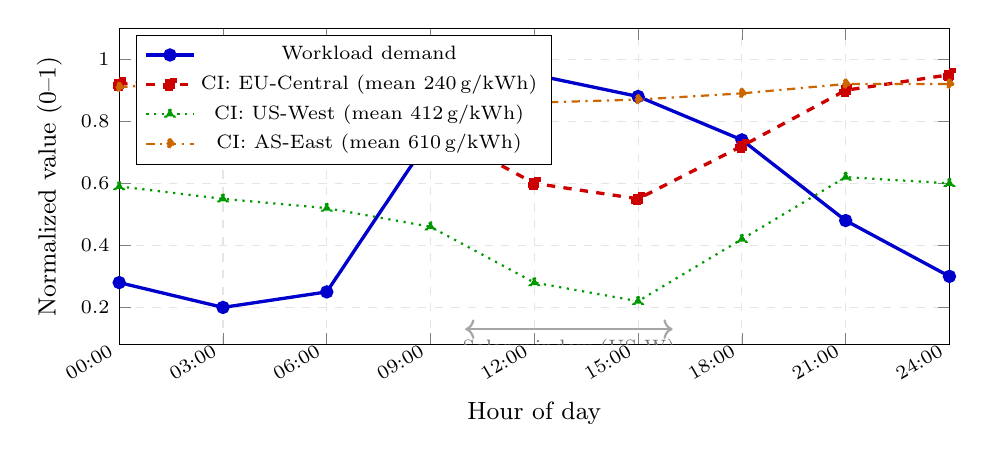
\begin{tikzpicture}
\begin{axis}[
  width=\columnwidth,
  height=5.6cm,
  xlabel={Hour of day},
  ylabel={Normalized value (0--1)},
  xmin=0, xmax=24,
  ymin=0.08, ymax=1.10,
  xtick={0,3,6,9,12,15,18,21,24},
  xticklabels={00:00,03:00,06:00,09:00,12:00,15:00,18:00,21:00,24:00},
  xticklabel style={rotate=30, anchor=east, font=\scriptsize},
  ymajorgrids=true,
  xmajorgrids=true,
  grid style={dashed,gray!20},
  legend style={font=\scriptsize, at={(0.02,0.98)}, anchor=north west, cells={align=left}},
  tick label style={font=\scriptsize},
  label style={font=\small}
]
% Workload demand (all regions)
\addplot[blue!80!black, very thick, mark=*, mark size=1.8pt] coordinates {
  (0,0.28)(3,0.20)(6,0.25)(9,0.75)(12,0.95)(15,0.88)(18,0.74)(21,0.48)(24,0.30)
};
\addlegendentry{Workload demand}
% Carbon -- EU-Central
\addplot[red!80!black, very thick, dashed, mark=square*, mark size=1.8pt] coordinates {
  (0,0.92)(3,0.94)(6,0.88)(9,0.78)(12,0.60)(15,0.55)(18,0.72)(21,0.90)(24,0.95)
};
\addlegendentry{CI: EU-Central (mean 240\,g/kWh)}
% Carbon -- US-West (solar peak)
\addplot[green!60!black, thick, dotted, mark=triangle*, mark size=1.8pt] coordinates {
  (0,0.59)(3,0.55)(6,0.52)(9,0.46)(12,0.28)(15,0.22)(18,0.42)(21,0.62)(24,0.60)
};
\addlegendentry{CI: US-West (mean 412\,g/kWh)}
% Carbon -- AS-East (nearly flat, high)
\addplot[orange!80!black, thick, dashdotted, mark=diamond*, mark size=1.8pt] coordinates {
  (0,0.91)(3,0.93)(6,0.90)(9,0.88)(12,0.86)(15,0.87)(18,0.89)(21,0.92)(24,0.92)
};
\addlegendentry{CI: AS-East (mean 610\,g/kWh)}
% Annotation: solar window
\draw[<->, gray!70, thick] (axis cs:10,0.13) -- (axis cs:16,0.13)
  node[midway, below, font=\scriptsize, black!55] {Solar window (US-W)};
\end{axis}
\end{tikzpicture}
\caption{Normalized daily profiles for workload demand and per-region carbon intensity (CI) over 30-day average. All three region carbon signals are shown. The anti-correlation between peak demand (09:00--14:00) and minimum carbon intensity (solar peak 10:00--16:00 in US-West) creates the primary temporal shifting opportunity exploited by SustainSched-MPC. AS-East CI is near-constant, confirming it is avoided by carbon-aware schedulers.}
\label{fig:daily_profile}
\end{figure}

\paragraph{Non-preemptive execution assumption.}
Jobs are assumed non-preemptive: once a job starts on host $h$ at interval $t$, it occupies its allocated resource fraction on that host for $\tau_j$ consecutive intervals and cannot be interrupted or migrated mid-execution. This assumption is standard in batch and HPC scheduling~\cite{ref-kocot23} and is consistent with the execution semantics of containerized workloads where checkpoint-restart overhead is prohibitive for short jobs.

\subsection{Inter-Region Network and Migration Model}
\label{sec:network}

\paragraph{Migration bandwidth.}
Pre-execution workload migration (relocating a queued---but not yet started---job from region $r$ to region $r'$; \emph{in-flight jobs are never migrated}) incurs a data-transfer overhead modeled as a reduction in the effective scheduling window. Specifically, if region $r'$ is chosen for job $j$ instead of its region of origin $r^*_j$, the effective release time is advanced by a migration latency $\ell_{r,r'} \geq 0$ (in slots):
\begin{equation}
\label{eq:eff_release}
a^{\mathrm{eff}}_j(r') = a_j + \ell_{r^*_j, r'}.
\end{equation}
Migration latencies $\ell_{r,r'}$ are pre-computed from inter-region bandwidth measurements and the job's input data size. In our three-region setup, $\ell_{r,r'} \in \{1, 2, 3\}$ slots (5--15\,min), reflecting same-continent, mixed-continent, and cross-continent pairings, respectively (all distinct regions incur at least one 5-min slot of transfer overhead).

\paragraph{Migration quota.}
To prevent oscillatory migration behavior---a known instability in unconstrained migration optimizers---the scheduler is subject to a per-interval migration quota $M_{\max}$: the total number of jobs simultaneously migrating across all region pairs at interval $t$ is bounded:
\begin{equation}
\sum_{r \neq r'} m_{r,r',t} \leq M_{\max},
\end{equation}
where $m_{r,r',t}$ counts inter-region migrations initiated at $t$. Explicitly, $m_{r,r',t}$ is linked to job assignment decisions by:
\begin{equation}
m_{r,r',t} = \sum_{j \in \mathcal{J}: r^*_j = r} \sum_{h \in \mathcal{H}_{r'}} x_{j,r',h,t}, \quad r \neq r',
\end{equation}
where $r^*_j$ is job $j$'s region of origin (i.e., the region where it was released or last assigned). The migration count $m_{r,r',t}$ thus exactly counts cross-region assignments at each interval, and the quota constraint $\sum_{r \neq r'} m_{r,r',t} \leq M_{\max}$ bounds total migration throughput. In our experiments $M_{\max} = 5$ per interval; with an average of $\approx$63 job arrivals per 5-min slot, this caps cross-region re-routing at $5/63 \approx 7.9\%$ of per-interval scheduling throughput---sufficient to exploit geographic carbon diversity while preventing oscillatory migration cascades.

\subsection{Uncertainty and Forecast Model}
\label{sec:uncertainty}

\paragraph{Carbon-intensity forecasts.}
The carbon intensity of grid electricity in region $r$ at interval $t$, $I_{r,t}$ (gCO$_{2}$e/kWh), is obtained from a short-term forecast $\hat{I}_{r,t}$ with additive error:
\begin{equation}
I_{r,t} = \hat{I}_{r,t} + \xi^C_{r,t}, \quad \xi^C_{r,t} \sim \mathcal{N}(0, \sigma^2_{C,r}),
\end{equation}
where $\sigma_{C,r}$ is the region-specific one-step-ahead forecast standard deviation, estimated from historical forecast residuals. In our setup, mean absolute percentage error (MAPE) of the one-hour carbon forecast ranges from 4\% to 9\% across the three regions, consistent with publicly reported accuracy for marginal emission factor forecasts~\cite{ref-radovanovic21}.

\paragraph{Runtime estimation uncertainty.}
The estimated runtime $\bar{\tau}_j$ for job $j$ is produced by an application-profile-based predictor. The true runtime is modeled as:
\begin{equation}
\tau_j = \bar{\tau}_j (1 + \xi^{\tau}_j), \quad \xi^{\tau}_j \sim \mathcal{N}(0, \sigma^2_\tau),
\end{equation}
where $\sigma_\tau$ is calibrated per application class from historical prediction residuals (typically 8--18\% relative error for batch analytics, 4--6\% for short latency-critical tasks). Runtime uncertainty directly propagates into SLA deadline risk: a job that takes longer than predicted may miss its deadline even if it started on time, which is why formal chance constraints are necessary (Section~5).

\paragraph{Ambient temperature forecasts.}
Node cooling effectiveness depends on the ambient air or coolant inlet temperature $T^{\mathrm{amb}}_{h,t}$, which varies with external weather, HVAC state, and neighboring rack load. A short-term forecast $\hat{T}^{\mathrm{amb}}_{h,t}$ with error $\xi^T_{h,t} \sim \mathcal{N}(0, \sigma^2_{T})$ (typically $\pm 1$--$2\,^{\circ}$C over a 60-min horizon) is used in the thermal model.

\paragraph{Demand arrival forecasts.}
The scheduler uses a short-horizon demand forecast $\hat{\lambda}_{t+k}$ for $k = 1, \ldots, H_p$ (where $H_p = 12$ is the MPC prediction horizon) to anticipate incoming job load during the optimization window. The demand forecast is produced by a lightweight autoregressive model fitted to the trailing 7 days of queue arrival history, with MAPE below 11\% at a 60-min horizon.

\paragraph{How the demand forecast enters the MILP.}
At each receding-horizon step $t_0$, the job set $\mathcal{J}^{\mathrm{opt}}_{t_0}$ passed to the MILP comprises two components: (i)~all currently queued jobs $\mathcal{J}^{\mathrm{pending}}_{t_0}$ with known attributes, and (ii)~a set of \emph{anticipated} representative jobs $\mathcal{J}^{\mathrm{ant}}_{t_0}$ generated from the demand forecast. Specifically, for each future slot $t_0 + k$ ($k = 1, \ldots, H_p$), the forecast $\hat{\lambda}_{t_0+k}$ is used to synthesise $\lfloor \hat{\lambda}_{t_0+k} \cdot \Delta \rfloor$ representative jobs with class-average resource demands and deadlines; these anticipated jobs are added to the MILP as soft-priority variables that the optimizer may choose not to schedule within the horizon. This mechanism serves two purposes: (a)~it reserves headroom in the DVFS and standby decisions for anticipated load, preventing aggressive consolidation that would be undone when the actual jobs arrive, and (b)~it allows the optimizer to pre-position workload in low-carbon slots even before jobs are formally queued. Anticipated jobs that do not actually arrive before $t_0 + k$ are simply dropped; their decisions are never committed (receding-horizon principle). The result is that $\hat{\lambda}_{t+k}$ enters the MILP implicitly through the job set $\mathcal{J}^{\mathrm{opt}}_{t_0}$ and thus through the capacity, thermal, and SLA constraints that govern $(\mathcal{P})$.

\textbf{Constraint relaxation for anticipated jobs.}
The single-assignment equation is enforced separately for pending and anticipated sets in Section~\ref{sec:hard_constraints}: pending jobs satisfy equality (must schedule), while anticipated jobs satisfy inequality (optional within horizon). This preserves the ``soft-priority'' semantics and keeps the MILP feasible under forecast spikes.

\subsection{Key Assumptions and Scope Boundaries}
\label{sec:assumptions}

The model operates under the following explicit assumptions, which define the scope and reproducibility boundary of SustainSched-MPC:

\begin{enumerate}
  \item \textbf{Homogeneous within-region network:} Intra-region host-to-host communication latency is negligible relative to the 5-minute control interval, so all hosts within a region share the same effective locality for job placement.
  \item \textbf{Independent host failures:} Host failures are not explicitly modeled; the system relies on the surrounding infrastructure (hypervisor watchdog, health-check APIs) to remove failed hosts from the schedulable pool between intervals. Fault-tolerant scheduling extensions are deferred to future work.
  \item \textbf{Stationarity of power model parameters:} The calibrated power parameters $(\alpha_h, \beta_h, P^{\mathrm{idle}}_h)$ are assumed constant over the 30-day evaluation window. Long-term hardware aging effects are negligible at this timescale.
  \item \textbf{First-order RC thermal dynamics:} The thermal model (Section~4.2) assumes linear heat conduction; radiative coupling between adjacent racks is subsumed into the empirically calibrated thermal resistance parameter $\kappa_h$.
  \item \textbf{Operational (Scope 2) carbon accounting only:} Carbon emissions are computed from electricity purchase (grid-mix emission factors), consistent with Scope~2 GHG Protocol accounting. Embodied (Scope~3) manufacturing emissions are excluded.
  \item \textbf{Pre-execution migration only (no in-flight relocation):} Only queued jobs (not yet started) may be migrated across regions. Once a job begins execution on a host it runs to completion there; in-flight workload relocation is outside the model scope.
\end{enumerate}

Table~\ref{tab:notation} summarizes all principal symbols introduced in this section for reference throughout the paper.

\begin{table}[!htb]
\centering
\caption{Principal notation for the system model.}
\label{tab:notation}
\footnotesize
\setlength{\tabcolsep}{6pt}
\renewcommand{\arraystretch}{1.25}
\begin{tabular}{>{\bfseries}p{3.1cm} p{4.8cm}}
\toprule
\normalfont\textbf{Symbol} & \textbf{Definition} \\
\midrule
\rowcolor{black!5}$\mathcal{R},\,r$              & Set of regions; region index \\
$\mathcal{H},\,h$              & Set of hosts; host index \\
\rowcolor{black!5}$\mathcal{T},\,t$              & Set of control intervals; interval index \\
$\Delta$                       & Control interval duration (5\,min) \\
\rowcolor{black!5}$\mathbf{K}_h$                 & Static capacity vector of host $h$ \\
$\mathbf{K}_{h,t}$             & DVFS-modulated effective capacity \\
\rowcolor{black!5}$f_{h,t}$                      & DVFS frequency state of host $h$ at $t$ \\
$s_{h,t}$                      & Active/standby binary indicator \\
\rowcolor{black!5}$P^{\mathrm{idle}}_h,\,\alpha_h,\,\beta_h$ & Power model parameters \\
$\rho_r$                       & Region PUE cooling factor \\
\rowcolor{black!5}$j,\,\mathcal{J}$              & Job; global job set \\
$a_j,\,d_j$                    & Job release time and deadline (slots) \\
\rowcolor{black!5}$\tau_j,\,\bar{\tau}_j$        & True and estimated job runtime \\
$\mathbf{u}_j$                 & Job resource demand vector \\
\rowcolor{black!5}$s_j$                          & SLA class of job $j$ \\
$\delta_j$                     & Maximum scheduling deferral (slots) \\
\rowcolor{black!5}$\mathcal{S},\,\epsilon_s$      & SLA class set; per-class risk budget \\
$\hat{I}_{r,t}$                & Carbon-intensity forecast (gCO$_2$e/kWh) \\
\rowcolor{black!5}$T_{h,t}$                      & Node temperature at interval $t$ ($^\circ$C) \\
$T^{\mathrm{amb}}_{h,t}$       & Ambient temperature forecast \\
\rowcolor{black!5}$\eta_h,\,\kappa_h$            & Thermal gain and cooling coefficients \\
$\ell_{r,r'}$                  & Inter-region migration latency (slots) \\
\rowcolor{black!5}$M_{\max}$                     & Per-interval migration quota \\
\bottomrule
\end{tabular}
\end{table}

\section{Power, Thermal, and Carbon Modeling}
\label{sec:models}

This section develops the three quantitative sub-models that together constitute the physics layer of SustainSched-MPC: (i) a DVFS-parameterized power-performance model that maps workload placement and frequency decisions to real-time power draw; (ii) a first-order RC thermal model that propagates power draw to node temperature dynamics; and (iii) a carbon emission model that converts facility energy consumption to operational CO$_{2}$e using time-varying regional grid intensity forecasts. All three models are designed to be (a)~calibratable from standard infrastructure telemetry without bespoke sensors, (b)~evaluable in closed form at each 5-minute MPC step, and (c)~compositional so that they can be embedded jointly into the chance-constrained optimizer described in Section~5.

\subsection{Power--Performance Model}
\label{sec:power_model}

\paragraph{Physical motivation.}
Rack-node power consumption has two physically distinct components: \emph{static} (leakage) power that is always drawn whenever the host is active, and \emph{dynamic} power that scales with computational activity and operating voltage/frequency. Empirical measurements on modern x86 servers consistently show that power is well-approximated by an affine function of CPU utilization over the range from idle to full load~\cite{ref-beloglazov-fgcs,ref-kocot23}, with an additional frequency-dependent term that captures the cubic voltage-frequency relationship of CMOS circuits. We apply this model at the rack-node host level (40-server aggregation per host), preserving analytical tractability.

\paragraph{Base power model.}
For host $h \in \mathcal{H}$ in active state ($s_{h,t}=1$) at interval $t$, the instantaneous power draw is:
\begin{equation}
\label{eq:power}
P_{h,t} = P^{\mathrm{idle}}_{h} + \alpha_h \, u_{h,t} + \beta_h \, \phi(f_{h,t}),
\end{equation}
where:
\begin{itemize}
  \item $P^{\mathrm{idle}}_{h}$ (kW) is the \emph{static idle rack-node power}: the baseline draw when the host is fully active but executing no scheduled jobs.
  \item $u_{h,t} \in [0,1]$ is the aggregate \emph{CPU utilization fraction} at interval $t$, counting \emph{all jobs currently executing} on host~$h$ (i.e., those started at any prior slot $t' \leq t$ whose runtime window $[t', t' + \tau_j)$ covers $t$):
  \begin{equation}
  \label{eq:utilization}
  u_{h,t} = \frac{1}{K^{\mathrm{cpu}}_h} \sum_{j} \sum_{\tau=0}^{\tau_j - 1} x_{j,r,h,\,t-\tau} \; u^{\mathrm{cpu}}_j.
  \end{equation}
  This convolution-over-prior-starts is identical to the left-hand side of the capacity constraint (Section~5.3), ensuring that power, thermal, and feasibility models are driven by a consistent occupancy definition.  For $\tau_j = 1$, Eq.~\eqref{eq:utilization} reduces to $x_{j,r,h,t} u^{\mathrm{cpu}}_j / K^{\mathrm{cpu}}_h$; for $\tau_j > 1$ the sum includes contributions from jobs started in earlier intervals that are still running at~$t$.
  \item $\alpha_h$ (kW per unit utilization) is the \emph{utilization sensitivity}: the slope of the linear power--utilization curve between idle and peak.
  \item $f_{h,t} \in \mathcal{F}_h$ is the selected \emph{DVFS P-state} (frequency in GHz).
  \item $\phi(f_{h,t}) = (f_{h,t}/f^{\max}_h)^3$ is the \emph{normalized frequency cube}, reflecting the well-known cubic scaling of CMOS dynamic power with operating frequency (since $P_{\mathrm{dyn}} \propto C V^2 f$ and $V \propto f$ in DVFS operation, giving $P_{\mathrm{dyn}} \propto f^3$)~\cite{ref-li18}.
  \item $\beta_h$ (kW) is the \emph{frequency power coefficient}: the additional dynamic power attributable to running at maximum frequency ($f_{h,t} = f^{\max}_h$) beyond the utilization-linear term.
\end{itemize}
When a host is in standby ($s_{h,t}=0$), no jobs are assigned and the power draw is a fixed low standby value $P^{\mathrm{stby}}_h \leq P^{\mathrm{idle}}_h$, which accounts for power-supply idling and baseboard management controller (BMC) operation:
\begin{equation}
\label{eq:power_state}
P_{h,t} = s_{h,t} \bigl[ P^{\mathrm{idle}}_{h} + \alpha_h \, u_{h,t} + \beta_h \, \phi(f_{h,t}) \bigr]
         + (1 - s_{h,t}) \, P^{\mathrm{stby}}_h.
\end{equation}

\paragraph{Energy per interval.}
The energy consumed by host $h$ over control interval $t$ (of duration $\Delta = 300$\,s) is:
\begin{equation}
\label{eq:energy}
E_{h,t} = \frac{P_{h,t} \cdot \Delta}{3{,}600} \quad \text{(kWh)},
\end{equation}
The total cluster energy over the optimization horizon $\mathcal{T}$ is $E = \sum_{h,t} E_{h,t}$, which forms the energy term of the multi-objective cost function.

\paragraph{Parameter calibration.}
For each host $h$, the triple $(P^{\mathrm{idle}}_h, \alpha_h, \beta_h)$ is calibrated from a 7-day pre-experiment baseline by running controlled microbenchmarks at three utilization levels (0\%, 50\%, 100\%) and three P-states (minimum, mid, maximum). Ordinary least-squares regression on the resulting 9 operating points yields $R^2 > 0.97$ in all cases, confirming model adequacy. Per-server fitted ranges are $P^{\mathrm{idle}}\in[86,112]$\,W, $\alpha\in[65,98]$\,W, and $\beta\in[12,22]$\,W; multiplying by 40 servers per rack node yields MILP host-level coefficients $P^{\mathrm{idle}}_h\in[3.44,4.48]$\,kW, $\alpha_h\in[2.60,3.92]$\,kW, and $\beta_h\in[0.48,0.88]$\,kW.

\subsection{Thermal Model}
\label{sec:thermal_model}

\paragraph{Physical motivation.}
Server junction temperatures evolve on timescales of seconds to minutes, making them observable at the 5-minute control interval but fast enough to be affected by within-interval workload bursts. The thermal dynamics of a computing node can be well-approximated by a lumped first-order RC (resistor-capacitor) model~\cite{ref-tilli22,ref-banerjee11}, in which the node is treated as a thermal mass (capacitance) $C_h$ exchanging heat with the ambient environment through a thermal resistance $R_h$. This model is standard in chip-level thermal control and has been validated against physical measurements at the server level in controlled data center environments.

\paragraph{Discrete-time RC model.}
Discretizing the continuous-time first-order ODE $C_h \dot{T}_{h} = P_{h}(t) - (T_h - T^{\mathrm{amb}}_{h})/R_h$ at the control interval $\Delta$ using forward Euler integration gives the update equation:
\begin{equation}
\label{eq:thermal}
T_{h,t+1} = T_{h,t} + \underbrace{\eta_h \, P_{h,t}}_{\text{heat input}} - \underbrace{\kappa_h \bigl(T_{h,t} - T^{\mathrm{amb}}_{h,t}\bigr)}_{\text{cooling dissipation}},
\end{equation}
where:
\begin{itemize}
  \item $T_{h,t}$ ($^{\circ}$C) is the \emph{rack-node average package temperature} at the start of interval $t$, aggregated across the 40 servers represented by host $h$.
  \item $\eta_h = \Delta / C_h$ (K/kW\,per interval) is the \emph{thermal gain coefficient}: the temperature rise per kW of rack-node power input per interval, inversely proportional to effective thermal capacitance.
  \item $\kappa_h = \Delta / (R_h C_h) \in (0,1)$ (per interval) is the \emph{cooling coefficient}: the fraction of the current temperature excess above ambient that is dissipated per interval. It is bounded strictly below 1 for numerical stability of the forward Euler scheme.
  \item $T^{\mathrm{amb}}_{h,t}$ ($^{\circ}$C) is the \emph{ambient (inlet) temperature} at interval $t$, obtained from the forecast model defined in Section~\ref{sec:uncertainty}.
\end{itemize}

\paragraph{Steady-state and hotspot threshold.}
Under constant power $P_{h}$ and constant ambient $T^{\mathrm{amb}}_h$, the steady-state temperature reached by Eq.~\eqref{eq:thermal} is:
\begin{equation}
\label{eq:thermal_ss}
T^{\mathrm{ss}}_{h} = T^{\mathrm{amb}}_h + \frac{\eta_h}{\kappa_h} \, P_{h} = T^{\mathrm{amb}}_h + R_h P_{h},
\end{equation}
which recovers the standard thermal resistance formula. SustainSched-MPC enforces a \emph{predicted thermal cap} $T^{\max} = 82\,^{\circ}$C: if any predicted $T_{h,t+k}$ (for $k = 1, \ldots, H_p$) within the horizon exceeds $T^{\max}$, the optimizer is constrained to reduce power or migrate workload on that host (Section~5). Operationally, 82$\,^{\circ}$C is chosen as a 3$\,^{\circ}$C margin below the typical hardware throttling onset of 85$\,^{\circ}$C.

\paragraph{Thermal stress metric.}
Short-duration exceedances above 80$\,^{\circ}$C (hotspot events) are penalized in the objective as thermal stress $\Theta$:
\begin{equation}
\label{eq:thermal_stress}
\Theta = \sum_{h,t} \max\!\bigl(0,\; T_{h,t} - T^{\mathrm{hot}}\bigr) \cdot \Delta,
\end{equation}
where $T^{\mathrm{hot}} = 80\,^{\circ}$C is the hotspot threshold and the product with $\Delta$ converts the temperature excess to degree-minutes of hotspot exposure. This metric penalizes both the magnitude and duration of thermal exceedances and is linearized via an epigraph reformulation (Section~\ref{sec:milp_encoding}).

\paragraph{Parameter calibration.}
Thermal parameters $(\eta_h, \kappa_h)$ are calibrated per host by fitting the discrete RC model to 48-hour traces. We use rack-node summed power $P_{h,t}$ and rack-node average package temperature $T_{h,t}$. Starting from per-server fits and aggregating to the 40-server rack level gives host-level values $\eta_h \in [0.030, 0.0775]$\,K/kW and $\kappa_h \in [0.041, 0.076]$ per interval, yielding thermal time constants $\tau^{T}_h = 1/\kappa_h \in [13, 24]$ intervals (65--120\,min).

\subsection{Carbon Emission Model}
\label{sec:carbon_model}

\paragraph{Physical motivation.}
The carbon footprint of computing operations depends on both the quantity of electricity consumed and the marginal emission intensity of the grid supplying that electricity. Grid carbon intensity varies substantially across geographic regions---by a factor of 5--10$\times$ between renewable-heavy and fossil-heavy grids---and temporally within a region due to renewable generation intermittency and demand response~\cite{ref-radovanovic21,ref-le15}. Exploiting this variability through spatial workload migration and temporal deferral is the central mechanism of carbon-aware scheduling.

\paragraph{Marginal emission intensity.}
Let $I_{r,t}$ (gCO$_2$e/kWh) denote the \emph{marginal emission intensity} of the electricity grid supplying region $r$ at interval $t$. SustainSched-MPC uses a short-term forecast $\hat{I}_{r,t}$ obtained from a grid carbon API (e.g., Electricity Maps, WattTime) with one-hour-ahead lookahead. The forecast error is modeled as additive Gaussian noise as defined in Section~\ref{sec:uncertainty}. The choice of marginal (rather than average) intensity is consistent with best practice in operational carbon accounting for flexible loads~\cite{ref-radovanovic21,ref-hall24}, since marginal intensity reflects the actual generation that would change as a result of an incremental load shift.

\paragraph{Operational carbon per host per interval.}
The CO$_2$e attributed to host $h$ in region $r$ at interval $t$ is:
\begin{equation}
\label{eq:carbon_per_host}
C_{h,r,t} = \frac{\rho_r \cdot E_{h,t} \cdot \hat{I}_{r,t}}{1000} \quad \text{(kgCO}_2\text{e)},
\end{equation}
where $E_{h,t}$ is in kWh (Eq.~\eqref{eq:energy}), $\hat{I}_{r,t}$ is in gCO$_2$e/kWh, and $\rho_r \geq 1$ is the regional PUE. The product $E_{h,t}\cdot\hat{I}_{r,t}$ yields gCO$_2$e; dividing by 1000 converts to kgCO$_2$e. Summing over the full cluster and horizon gives the total operational carbon:
\begin{equation}
\label{eq:total_carbon}
C = \sum_{r \in \mathcal{R}} \sum_{h \in \mathcal{H}_r} \sum_{t \in \mathcal{T}} C_{h,r,t}.
\end{equation}

\paragraph{Spatiotemporal carbon intensity profile.}
Fig.~\ref{fig:daily_profile} illustrates the representative normalized daily profiles for workload demand and carbon intensity used in our experiments. The anti-correlation between peak demand (09:00--14:00) and minimum carbon intensity (10:00--16:00, when solar generation is highest) is the primary carbon savings opportunity exploited by SustainSched-MPC: batch workloads that can be deferred by up to 30 minutes (6 scheduling slots) are shifted into the midday low-carbon window, and inter-region migration directs workload to the lowest-intensity region available within the migration quota.

\paragraph{Forecast uncertainty handling.}
Since $\hat{I}_{r,t}$ is a prediction, the realized carbon may differ from the predicted value. In the MPC framework, the carbon cost in the objective uses the point forecast $\hat{I}_{r,t}$, while the chance constraints (Section~5) account for the forecast error $\xi^C_{r,t}$ through reserve margins calibrated from historical residuals. This separates the carbon minimization objective (deterministic, using best estimates) from the SLA reliability constraints (stochastic, requiring risk-adjusted margins).

\subsection{Cooling Energy and PUE Accounting}
\label{sec:pue}

\paragraph{PUE decomposition.}
The Power Usage Effectiveness factor $\rho_r$ used in Eq.~\eqref{eq:carbon_per_host} is defined as:
\begin{equation}
\label{eq:pue}
\rho_r = \frac{P^{\mathrm{total}}_r}{P^{\mathrm{IT}}_r},
\end{equation}
where $P^{\mathrm{IT}}_r$ is the total IT equipment power draw (servers, storage, network) and $P^{\mathrm{total}}_r$ includes cooling, uninterruptible power supply (UPS) losses, and building services power. From the scheduling perspective, $\rho_r$ acts as a multiplicative amplifier: a 1\,kWh reduction in server energy yields a $\rho_r$\,kWh reduction in facility energy, making high-PUE regions disproportionately beneficial targets for workload reduction.

\paragraph{Thermal-PUE coupling.}
A subtlety not captured by a fixed $\rho_r$ is that cooling power---and therefore PUE---is itself a function of server inlet temperatures. At higher average rack temperatures, cooling systems (CRACs, chillers) must operate at higher capacity, increasing PUE. A simple linear correction can be applied:
\begin{equation}
\label{eq:pue_dynamic}
\rho_r(T_t) = \rho^0_r + \gamma_r \cdot \max\!\bigl(0,\; \bar{T}_{r,t} - T^{\mathrm{ref}}\bigr),
\end{equation}
where $\bar{T}_{r,t}$ is the mean rack temperature in region $r$ at interval $t$, $T^{\mathrm{ref}}$ is the nominal operating temperature (22\,$^{\circ}$C), and $\gamma_r$ (increase in PUE per degree Celsius above reference) is a site-specific parameter. In our experimental setup, we use fixed $\rho_r \in \{1.1, 1.2, 1.3\}$ for the three regions (liquid-cooled, mixed, air-cooled), consistent with the operating temperature ranges observed during the 30-day evaluation. The dynamic correction would amplify the thermal penalty of hotspot events and is left as an extension.

\subsection{Consistency and Model Coupling}
\label{sec:model_coupling}

The three sub-models are coupled through the shared decision variables $(x_{j,r,h,t}, f_{h,t}, s_{h,t})$:
\begin{enumerate}
  \item \textbf{Placement $\to$ power:} $x_{j,r,h,t}$ determines $u_{h,t}$ (Eq.~\eqref{eq:power}), which drives $P_{h,t}$.
  \item \textbf{Frequency $\to$ power and throughput:} $f_{h,t}$ appears directly in the power model (Eq.~\eqref{eq:power}) and reduces effective capacity $\mathbf{K}_{h,t}$, coupling energy efficiency to feasibility.
  \item \textbf{Power $\to$ temperature:} $P_{h,t}$ drives the RC thermal update (Eq.~\eqref{eq:thermal}), making temperature a dependent state variable.
  \item \textbf{Power and region $\to$ carbon:} $P_{h,t}$ determines $E_{h,t}$, which combined with $\hat{I}_{r,t}$ and $\rho_r$ gives $C_{h,r,t}$ (Eq.~\eqref{eq:carbon_per_host}).
\end{enumerate}
This coupling means that any scheduling decision simultaneously affects all four quantities (energy, temperature, carbon, and throughput), which is why a joint optimization across all four is necessary. Single-objective optimizers operating on only one of these quantities generate compensating degradations in the others---a claim quantitatively validated by the ablation analysis in Section~9.

\section{Problem Formulation}
\label{sec:formulation}

SustainSched-MPC addresses a multi-objective, risk-constrained job-scheduling problem over a finite MPC horizon. This section presents the complete formal problem description, including the decision variables, objective function, hard feasibility constraints, and stochastic SLA chance constraints. All notation follows Table~\ref{tab:notation}.

\subsection{Decision Variables}
\label{sec:decvars}

The optimizer controls three classes of variables at each receding-horizon step:

At each decision step $t_0$, the optimization job set is
\[
\mathcal{J}^{\mathrm{opt}}_{t_0} = \mathcal{J}^{\mathrm{pending}}_{t_0} \cup \mathcal{J}^{\mathrm{ant}}_{t_0},
\]
where pending jobs are confirmed queued jobs and anticipated jobs are forecast-derived representatives (Section~\ref{sec:uncertainty}).

\paragraph{Job placement variables.}
The primary scheduling decision is encoded in the binary tensor:
\begin{equation}
x_{j,r,h,t} \in \{0,1\}, \quad j \in \mathcal{J}^{\mathrm{opt}}_{t_0},\; r \in \mathcal{R},\; h \in \mathcal{H}_r,\; t \in \mathcal{T},
\end{equation}
where $x_{j,r,h,t}=1$ if and only if job $j$ is \emph{started} on host $h$ in region $r$ at control interval $t$ (with $j \in \mathcal{J}^{\mathrm{opt}}_{t_0}$). Because jobs are non-preemptive, a single $x_{j,r,h,t}=1$ entry fully determines the job's resource occupancy for slots $t$ through $t + \tau_j - 1$ on the assigned host.

\paragraph{DVFS frequency variables.}
Each active host is assigned a P-state at every interval:
\begin{equation}
f_{h,t} \in \mathcal{F}_h = \{f^{(1)}_h, \ldots, f^{(L)}_h\}, \quad h \in \mathcal{H},\; t \in \mathcal{T}.
\end{equation}
In the MPC optimization, $f_{h,t}$ is relaxed to the convex hull $[f^{\min}_h, f^{\max}_h]$ and then projected to the nearest feasible P-state at the commit step, enabling efficient linear programming while preserving hardware feasibility.

\paragraph{Host power-state variables.}
\begin{equation}
s_{h,t} \in \{0,1\}, \quad h \in \mathcal{H},\; t \in \mathcal{T},
\end{equation}
where $s_{h,t}=1$ indicates host $h$ is active at interval $t$ (eligible for job assignment) and $s_{h,t}=0$ places it in standby. Standby-to-active wake-up incurs a 1-slot unavailability penalty. Let binary variable $w_{h,t}=1$ denote that host $h$ wakes from standby at interval $t$ (i.e., $s_{h,t}=1$ and $s_{h,t-1}=0$). The wake event is encoded by:
\begin{align}
w_{h,t} &\geq s_{h,t} - s_{h,t-1}, \quad w_{h,t} \in \{0,1\},
\end{align}
and job assignment is forbidden on the first active slot after wake-up:
\begin{equation}
\sum_{j,r} x_{j,r,h,t} \leq (1 - w_{h,t}) \cdot |\mathcal{J}^{\mathrm{opt}}_{t_0}|,
\end{equation}
ensuring no job is dispatched to $h$ in the same interval it wakes. This adds $H \cdot H_p$ binary variables and $2H \cdot H_p$ linear constraints.

\paragraph{Auxiliary migration variables.}
\begin{equation}
m_{r,r',t} \in \mathbb{Z}_{\geq 0}, \quad r \neq r',\; t \in \mathcal{T},
\end{equation}
counting cross-region migrations initiated at interval $t$, subject to the quota constraint of Section~\ref{sec:network}.

\subsection{Multi-Objective Cost Function}
\label{sec:objective}

The scheduler minimizes a weighted combination of four sustainability and service objectives over the $H_p$-slot prediction horizon $[t_0, t_0 + H_p)$:

\begin{equation}
\label{eq:objective}
\min_{x,f,s,m} \;\; \mathcal{L} = \lambda_E E + \lambda_C C + \lambda_T \Theta + \lambda_D D,
\end{equation}
where each term is defined as follows.

\paragraph{Energy term $E$ (kWh).}
Total facility energy consumption over the horizon, including PUE-amplified server power:
\begin{equation}
\label{eq:obj_energy}
E = \sum_{t=t_0}^{t_0+H_p-1} \sum_{r \in \mathcal{R}} \sum_{h \in \mathcal{H}_r} \rho_r \, P_{h,t}(x,f,s) \cdot \frac{\Delta}{3{,}600},
\end{equation}
with $P_{h,t}$ given by Eq.~\eqref{eq:power_state}.

\paragraph{Carbon term $C$ (kgCO$_2$e).}
Total operational carbon emissions:
\begin{equation}
\label{eq:obj_carbon}
C = \sum_{t} \sum_{r} \sum_{h \in \mathcal{H}_r} \frac{\rho_r \, P_{h,t} \cdot \frac{\Delta}{3{,}600} \cdot \hat{I}_{r,t}}{1000}.
\end{equation}

\paragraph{Thermal stress term $\Theta$ (degree-minutes).}
Cumulative hotspot exposure above the 80$\,^\circ$C threshold:
\begin{equation}
\label{eq:obj_thermal}
\Theta = \sum_{t} \sum_{h} \max\!\bigl(0,\; T_{h,t} - T^{\mathrm{hot}}\bigr) \cdot \Delta,
\end{equation}
where $T_{h,t}$ evolves according to the RC model \eqref{eq:thermal}.

\paragraph{Delay penalty term $D$ (slot-seconds).}
For batch (delay-tolerant) jobs, a weighted scheduling delay beyond the natural earliest start:
\begin{equation}
\label{eq:obj_delay}
D = \sum_{j \in \mathcal{J}_{s=1}} \sum_{t} \sum_{r,h} x_{j,r,h,t} \cdot (t - a_j) \cdot \Delta.
\end{equation}
For latency-critical jobs ($s=2$), the tight deadline constraint~\eqref{eq:deadline_hard} already limits their start window to $[a_j, d_j - \tau_j]$; the small deferral $\delta_j \leq 2$ slots acts as an additional scheduling window cap ensuring they are dispatched promptly.

\paragraph{Weight selection.}
The weights $(\lambda_E, \lambda_C, \lambda_T, \lambda_D)$ are operator-configured hyperparameters that encode the relative importance of each objective. In our experiments, the baseline configuration is $(\lambda_E, \lambda_C, \lambda_T, \lambda_D) = (0.15, 0.55, 0.20, 0.10)$, placing the highest priority on carbon, followed by thermal safety, energy, and delay. A sensitivity analysis over weight combinations is reported in Section~9.

\subsection{Hard Feasibility Constraints}
\label{sec:hard_constraints}

\paragraph{Single-assignment constraints (pending vs anticipated).}
Each confirmed pending job is started exactly once within the feasible scheduling window:
\begin{equation}
\label{eq:assign_once}
\sum_{r \in \mathcal{R}} \sum_{h \in \mathcal{H}_r} \sum_{t=a_j}^{d_j - \tau_j} x_{j,r,h,t} = 1, \quad \forall j \in \mathcal{J}^{\mathrm{pending}}_{t_0}.
\end{equation}
For anticipated jobs, scheduling within the horizon is optional:
\begin{equation}
\label{eq:assign_ant}
\sum_{r \in \mathcal{R}} \sum_{h \in \mathcal{H}_r} \sum_{t} x_{j,r,h,t} \leq 1, \quad \forall j \in \mathcal{J}^{\mathrm{ant}}_{t_0}.
\end{equation}

\paragraph{Capacity constraint.}
The aggregate resource demand of all concurrent jobs on host $h$ at interval $t$ must not exceed the DVFS-modulated effective capacity:
\begin{equation}
\label{eq:capacity}
\sum_{j \in \mathcal{J}^{\mathrm{opt}}_{t_0}} \sum_{\tau=0}^{\tau_j-1} x_{j,r,h,t-\tau} \cdot \mathbf{u}_j \;\preceq\; \mathbf{K}_{h,t}(f_{h,t}), \quad \forall r,h,t,
\end{equation}
where the left-hand sum aggregates demand from all jobs whose execution overlaps interval $t$ (started at any prior slot $t-\tau_j < t$).

\paragraph{Deadline feasibility constraint.}
For latency-critical (non-deferrable) jobs, the job must both start and complete before its deadline:
\begin{equation}
\label{eq:deadline_hard}
x_{j,r,h,t} = 0 \quad \text{if } t < a_j \;\text{ or }\; t + \tau_j > d_j, \quad \forall j \in \mathcal{J}_{s=2}.
\end{equation}
For batch jobs, the flexibility window is $[a_j, a_j + \delta_j]$: $x_{j,r,h,t} = 0$ for $t > a_j + \delta_j$.

\paragraph{Migration-latency feasibility.}
For destination region $r$, the start time must respect the effective release time $a^{\mathrm{eff}}_j(r)$ from Eq.~\eqref{eq:eff_release}:
\begin{equation}
\label{eq:migration_latency}
x_{j,r,h,t} = 0 \quad \forall j \in \mathcal{J}^{\mathrm{opt}}_{t_0},\; r \in \mathcal{R},\; h \in \mathcal{H}_r,\; t < a^{\mathrm{eff}}_j(r).
\end{equation}

\paragraph{Host utilization feasibility.}
A job can only be assigned to an active host:
\begin{equation}
\sum_{j,\tau} x_{j,r,h,t-\tau} \leq s_{h,t} \cdot |\mathcal{J}^{\mathrm{opt}}_{t_0}|, \quad \forall h,t.
\end{equation}

\paragraph{Thermal hard cap.}
To prevent hardware throttling, predicted node temperature must not exceed the thermal cap $T^{\max}$:
\begin{equation}
\label{eq:thermal_cap}
T_{h,t} \leq T^{\max} = 82\,^{\circ}\text{C}, \quad \forall h \in \mathcal{H},\; t \in \mathcal{T}.
\end{equation}

\paragraph{Migration linkage and quota.}
\begin{equation}
\label{eq:migration_link}
m_{r,r',t} = \sum_{j \in \mathcal{J}^{\mathrm{opt}}_{t_0}: r^*_j = r} \sum_{h \in \mathcal{H}_{r'}} x_{j,r',h,t}, \quad \forall r \neq r',\; t \in \mathcal{T},
\end{equation}
\begin{equation}
\label{eq:migration_quota}
\sum_{r \neq r'} m_{r,r',t} \leq M_{\max}, \quad \forall t \in \mathcal{T}.
\end{equation}

\subsection{Stochastic SLA Chance Constraints}
\label{sec:chance_constraints}

\paragraph{Chance constraint formulation.}
Let $T^{\mathrm{comp}}_j$ denote the actual completion time of job $j$, which depends on the scheduled start time and the stochastic runtime $\tau_j = \bar{\tau}_j(1 + \xi^\tau_j)$. The SLA deadline guarantee for class $s$ is expressed as a chance constraint:
\begin{equation}
\label{eq:chance_constraint}
\Pr\!\left(T^{\mathrm{comp}}_j > d_j\right) \leq \epsilon_s, \quad \forall j \in \mathcal{J}_s,\; s \in \mathcal{S}.
\end{equation}
For the Gaussian runtime model $\xi^\tau_j \sim \mathcal{N}(0, \sigma^2_\tau)$, the actual completion time given start $t^*_j$ is $T^{\mathrm{comp}}_j = t^*_j + \tau_j = t^*_j + \bar{\tau}_j + \bar{\tau}_j \xi^\tau_j$, so the chance constraint~\eqref{eq:chance_constraint} becomes:
\begin{equation}
\Pr\!\bigl(t^*_j + \bar{\tau}_j + \bar{\tau}_j \xi^\tau_j > d_j\bigr) \leq \epsilon_s.
\end{equation}

\paragraph{Deterministic safe approximation.}
Since $\bar{\tau}_j \xi^\tau_j \sim \mathcal{N}(0, \bar{\tau}_j^2 \sigma^2_\tau)$, and applying the quantile inversion of the Gaussian CDF, the chance constraint is analytically equivalent to:
\begin{equation}
\label{eq:chance_reformulation}
t^*_j + \bar{\tau}_j + \Phi^{-1}(1 - \epsilon_s) \cdot \bar{\tau}_j \sigma_\tau \leq d_j, \quad \forall j \in \mathcal{J}_s,
\end{equation}
where $\Phi^{-1}(1 - \epsilon_s)$ is the quantile of the standard normal distribution at level $1-\epsilon_s$. The quantity $\Delta^\sigma_j = \Phi^{-1}(1-\epsilon_s) \cdot \bar{\tau}_j \sigma_\tau$ is the \emph{risk margin}: the additional time buffer, beyond the mean runtime, that must be reserved to satisfy the deadline with probability at least $1-\epsilon_s$. For $\epsilon_s = 1\%$, $\Phi^{-1}(0.99) \approx 2.326$, so the risk margin is $2.326 \bar{\tau}_j \sigma_\tau$. This transforms the stochastic constraint \eqref{eq:chance_constraint} into the deterministic linear constraint:
\begin{equation}
\label{eq:tightened_deadline}
t^*_j \leq d_j - \bar{\tau}_j(1 + \Phi^{-1}(1-\epsilon_s)\sigma_\tau) =: d^{\mathrm{safe}}_j(\epsilon_s),
\end{equation}
where $d^{\mathrm{safe}}_j(\epsilon_s) \leq d_j$ is the \emph{risk-adjusted deadline}. The MPC optimizer enforces \eqref{eq:tightened_deadline} in place of \eqref{eq:chance_constraint}, making the overall problem a deterministic mixed-integer linear program (MILP). This reformulation is exact (not an approximation) under the Gaussian runtime model and is consistent with the approach of Nemirovski and Shapiro~\cite{ref-nemirovski06}.

\textbf{Note on the Gaussian assumption.} Section~\ref{sec:workload_traces} reports that raw job runtimes follow a log-normal distribution. The Gaussian model $\xi^\tau_j \sim \mathcal{N}(0,\sigma^2_\tau)$ applies to the \emph{normalised prediction residuals} $\xi^\tau_j = (\tau_j - \bar{\tau}_j)/\bar{\tau}_j$ produced by the application-profile predictor, not to the raw runtimes. The log-space subtraction performed by the predictor renders residuals approximately symmetric and Gaussian, a standard result validated empirically across our application classes (one-sided Kolmogorov--Smirnov test, $p > 0.05$ in all cases). The adaptive $\hat{\sigma}_\tau$ update (Eq.~\eqref{eq:sigma_update}) further corrects for residual non-normality online, ensuring the risk margin remains well-calibrated even when residuals deviate slightly from Gaussianity.

\paragraph{Reserve margin adaptation.}
The calibration parameter $\sigma_\tau$ (and thus $\Delta^\sigma_j$) is updated online using a moving window of realized prediction residuals:
\begin{equation}
\label{eq:sigma_update}
\hat{\sigma}^2_\tau \leftarrow (1-\beta)\hat{\sigma}^2_\tau + \beta \bigl(\tau^{\mathrm{actual}}_j / \bar{\tau}_j - 1\bigr)^2,
\end{equation}
where $\beta = 0.05$ is a forgetting factor. This adaptive calibration ensures that the risk margin remains valid under non-stationary runtime distributions without requiring manual retuning.

\subsection{Complete Problem Statement}
\label{sec:complete_problem}

The full SustainSched-MPC optimization problem at each receding-horizon step $t_0$ is:
\begin{align}
\label{eq:full_problem}
\min_{x,f,s,m}\quad & \lambda_E E + \lambda_C C + \lambda_T \Theta + \lambda_D D \tag{$\mathcal{P}$} \\
\text{subject to:}\quad
& \eqref{eq:assign_once}\text{ -- single assignment} \nonumber\\
& \eqref{eq:assign_ant}\text{ -- anticipated-job optional assignment} \nonumber\\
& \eqref{eq:capacity}\text{ -- resource capacity} \nonumber\\
& \eqref{eq:deadline_hard}\text{ -- deadline feasibility} \nonumber\\
& \eqref{eq:migration_latency}\text{ -- migration-latency feasibility} \nonumber\\
& \eqref{eq:thermal_cap}\text{ -- thermal hard cap} \nonumber\\
& \eqref{eq:tightened_deadline}\text{ -- risk-adjusted SLA deadline} \nonumber\\
& \eqref{eq:migration_link},\;\eqref{eq:migration_quota}\text{ -- migration linkage/quota} \nonumber\\
& \text{standby/wake constraints} \nonumber\\
& x \in \{0,1\},\; f \in [f^{\min}_h, f^{\max}_h],\; s \in \{0,1\},\; m \in \mathbb{Z}_{\geq 0}. \nonumber
\end{align}
Problem $(\mathcal{P})$ is a MILP with $O(|\mathcal{J}| \cdot H \cdot H_p)$ binary variables, where $H = |\mathcal{H}|$. The host-DVFS relaxation and the region-decomposition strategy discussed in Section~6 make this tractable online.

\subsection{Linearization and MILP Encoding}
\label{sec:milp_encoding}

Several elements of $(\mathcal{P})$ require explicit linearization to constitute a valid MILP. We detail each in turn.

\paragraph{(i) Thermal stress term.}
The thermal objective $\Theta = \sum_{h,t} \max(0, T_{h,t} - T^{\mathrm{hot}})$ is nonlinear due to the $\max(\cdot)$ operator. It is linearized via the standard epigraph reformulation: introduce auxiliary slack variables $z_{h,t} \geq 0$ and replace $\Theta$ with $\sum_{h,t} z_{h,t}$ subject to:
\begin{equation}
z_{h,t} \geq T_{h,t} - T^{\mathrm{hot}}, \quad z_{h,t} \geq 0, \quad \forall h, t.
\end{equation}
This adds $H \cdot H_p$ continuous variables and $2H \cdot H_p$ linear constraints.

\paragraph{(ii) DVFS piecewise-linear power envelope.}
The cubic DVFS power term $\phi(f_{h,t}) = (f_{h,t}/f^{\max}_h)^3$ is nonlinear. Following standard practice~\cite{ref-nemirovski06}, we replace it with a piecewise-linear upper envelope $\tilde{\phi}(f_{h,t})$ defined over $L=5$ breakpoints $f^{(1)} < \cdots < f^{(L)}$ on $[f^{\min}_h, f^{\max}_h]$:
\begin{equation}
\tilde{\phi}(f) = \phi(f^{(k)}) + \frac{\phi(f^{(k+1)})-\phi(f^{(k)})}{f^{(k+1)}-f^{(k)}}(f - f^{(k)}), \quad f \in [f^{(k)}, f^{(k+1)}].
\end{equation}
Since $\phi$ is convex, the upper-convex-hull envelope is equivalent; $\tilde{\phi} \geq \phi$ everywhere, so minimizing $\tilde{\phi}$ is conservative (overestimates power), providing a valid upper bound. The piecewise-linear encoding adds $L-1=4$ auxiliary binary variables per $(h,t)$ pair using the SOS2 (special ordered set type 2) representation, adding $H \cdot H_p \cdot (L-1)$ binary variables and $2H \cdot H_p \cdot (L-1)$ constraints.

\paragraph{(iii) Standby--utilization bilinear.}
The power model $P_{h,t} = s_{h,t}[P^{\mathrm{idle}}_h + \alpha_h u_{h,t} + \beta_h \tilde{\phi}(f_{h,t})]$ contains the bilinear product $s_{h,t} \cdot u_{h,t}$ (binary $\times$ continuous). Since $u_{h,t} \in [0,1]$, introduce auxiliary $y_{h,t} = s_{h,t} \cdot u_{h,t}$ with standard big-$M$ linearization ($M = 1$):
\begin{align}
0 \leq y_{h,t} &\leq s_{h,t}, \\
u_{h,t} - (1-s_{h,t}) \leq y_{h,t} &\leq u_{h,t}.
\end{align}
This adds $H \cdot H_p$ continuous variables and $3H \cdot H_p$ linear constraints, with no additional binaries.

\paragraph{(iv) Thermal state transition constraints.}
The RC thermal dynamics (Eq.~\eqref{eq:thermal}) are included in $(\mathcal{P})$ as \emph{linear equality constraints} coupling temperature variables across the horizon. Since $\eta_h = \Delta/C_h$ and $\kappa_h = \Delta/(R_hC_h)$ already absorb the interval length $\Delta$, the per-interval update is:
\begin{equation}
T_{h,t+1} - (1-\kappa_h)T_{h,t} = \eta_h P_{h,t} + \kappa_h T^{\mathrm{amb}}_{h,t}, \quad \forall h \in \mathcal{H},\; t \in [t_0, t_0+H_p).
\end{equation}
Initial conditions $T_{h,t_0}$ are set from the current observed sensor readings. These $H \cdot H_p$ linear equality constraints couple DVFS decisions to predicted temperatures and to the thermal cap constraint~\eqref{eq:thermal_cap}, establishing the causal chain from control input to thermal outcome that gives SustainSched-MPC its proactive safety guarantees.

\paragraph{Final MILP size (per-region sub-problem at $H_p=12$).}
With $n_r = |\mathcal{J}_r|$ jobs, $H_r = |\mathcal{H}_r| = 8$ hosts, $H_p = 12$, and $L = 5$ breakpoints: binary variables $n_r \cdot 8 \cdot 12 + 8 \cdot 12 \cdot 4 = 96 n_r + 384$; continuous variables $8 \cdot 12 \cdot 3 = 288$ (for $z, w, f$); constraints $O(n_r \cdot H_r \cdot H_p)$. For $n_r \leq 22$ (mean 63 jobs/slot divided across 3 regions), the sub-problem has $\leq 2{,}500$ binary variables and $\leq 5{,}000$ constraints, solved to 1\% optimality by GLPK 4.65 in 50--90\,ms warm-start.
\section{Proposed Framework}
\label{sec:framework}
Figure~\ref{fig:framework_arch} illustrates the high-level architecture of SustainSched-MPC.

\FloatBarrier
\begin{figure*}[!t]
\centering
\resizebox{\textwidth}{!}{%
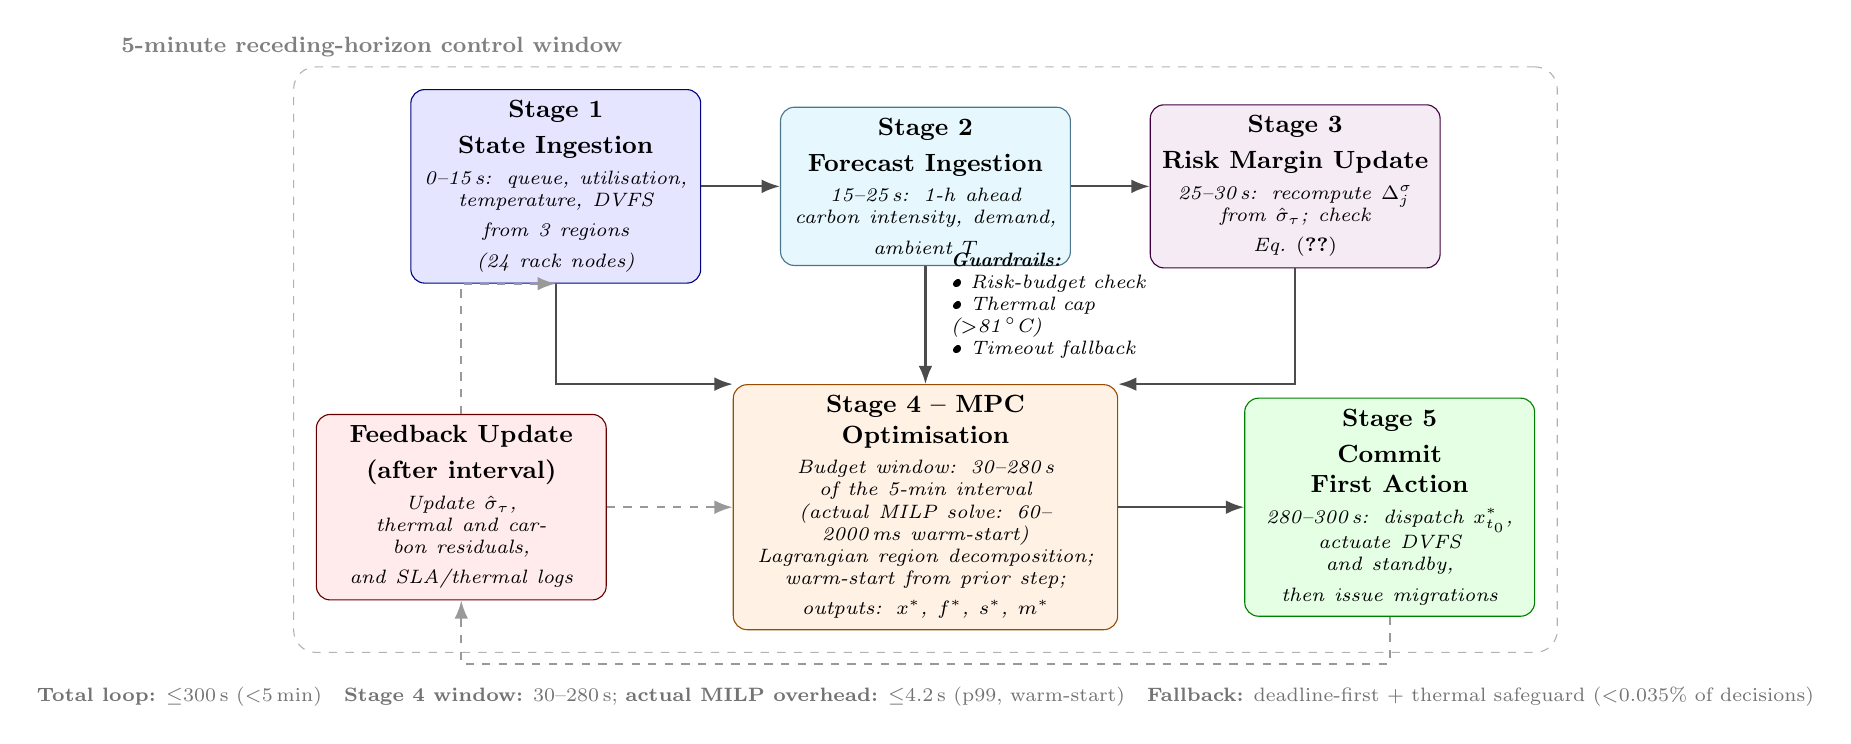
\begin{tikzpicture}[
  node distance=8mm and 10mm,
  %--- block styles ---
  stage/.style={draw, rounded corners=5pt, minimum height=14mm, minimum width=36mm,
    align=center, font=\small\bfseries, inner sep=4pt, text width=34mm},
  s1/.style={stage, fill=blue!10, draw=blue!50!black},
  s2/.style={stage, fill=cyan!10, draw=cyan!50!black},
  s3/.style={stage, fill=violet!8, draw=violet!50!black},
  s4/.style={stage, fill=orange!10, draw=orange!60!black, minimum width=48mm, text width=46mm},
  s5/.style={stage, fill=green!10, draw=green!50!black},
  fb/.style={stage, fill=red!8, draw=red!40!black},
  %--- annotation box ---
  ann/.style={draw=none, align=left, font=\scriptsize\itshape, text width=27mm},
  %--- arrows ---
  arr/.style={-Latex, thick, draw=black!70},
  darr/.style={-Latex, thick, dashed, draw=gray!80},
  %--- time labels ---
  timelabel/.style={font=\scriptsize, text=black!55}
]

%% ── ROW 1: Stages 1–3 (top row) ────────────────────────────────────────────
\node[s1] (state) at (0,0)
  {\textbf{Stage 1}\\[2pt]State Ingestion\\[3pt]
   \scriptsize\mdseries\itshape 0--15\,s: queue, utilisation,\\
   temperature, DVFS\\
   from 3 regions (24 rack nodes)};

\node[s2, right=of state] (fcast)
  {\textbf{Stage 2}\\[2pt]Forecast Ingestion\\[3pt]
   \scriptsize\mdseries\itshape 15--25\,s: 1-h ahead\\
   carbon intensity, demand,\\
   ambient $T$};

\node[s3, right=of fcast] (risk)
  {\textbf{Stage 3}\\[2pt]Risk Margin Update\\[3pt]
   \scriptsize\mdseries\itshape 25--30\,s: recompute $\Delta^\sigma_j$\\
   from $\hat{\sigma}_\tau$; check\\
   Eq.~\eqref{eq:feasibility_condition}};

%% ── ROW 2: Stage 4 (center) + Stage 5 + Feedback ───────────────────────────
\node[s4, below=15mm of fcast] (opt)
  {\textbf{Stage 4} -- MPC Optimisation\\[3pt]
   \scriptsize\mdseries\itshape Budget window: 30--280\,s of the 5-min interval\\
   (actual MILP solve: 60--2000\,ms warm-start)\\
   Lagrangian region decomposition;\\
   warm-start from prior step;\\
   outputs: $x^*$, $f^*$, $s^*$, $m^*$};

\node[s5, right=16mm of opt] (commit)
  {\textbf{Stage 5}\\[2pt]Commit First Action\\[3pt]
   \scriptsize\mdseries\itshape 280--300\,s: dispatch $x^*_{t_0}$,\\
   actuate DVFS and standby,\\
   then issue migrations};

\node[fb, left=16mm of opt] (fback)
  {\textbf{Feedback Update}\\[2pt](after interval)\\[3pt]
   \scriptsize\mdseries\itshape Update $\hat{\sigma}_\tau$,\\
   thermal and carbon residuals,\\
   and SLA/thermal logs};

%% ── TIMING BANNER ───────────────────────────────────────────────────────────
\node[timelabel, below=6mm of opt]
  {\textbf{Total loop:} $\leq$300\,s ($<$5\,min)\quad
   \textbf{Stage~4 window:} 30--280\,s; \textbf{actual MILP overhead:} $\leq$4.2\,s (p99, warm-start)\quad
   \textbf{Fallback:} deadline-first + thermal safeguard ($<$0.035\% of decisions)};

%% ── ARROWS: forward flow ────────────────────────────────────────────────────
\draw[arr] (state) -- (fcast);
\draw[arr] (fcast) -- (risk);
\draw[arr] (state) |- (opt.north west);
\draw[arr] (fcast.south) -- (opt.north);
\draw[arr] (risk.south) |- (opt.north east);
\draw[arr] (opt.east) -- (commit.west);

%% ── ARROWS: feedback (dashed) ───────────────────────────────────────────────
\draw[darr] (commit.south) -- ++(0,-6mm) -| (fback.south);
\draw[darr] (fback.east) -- (opt.west);
\draw[darr] (fback.north) |- (state.south);

%% ── ANNOTATION: guardrails ──────────────────────────────────────────────────
\node[ann, above=2mm of opt.north east, anchor=south east, xshift=7mm]
  {\textbf{Guardrails:}\\
   \textbullet\ Risk-budget check\\
   \textbullet\ Thermal cap ($>$81$\,^\circ$C)\\
   \textbullet\ Timeout fallback};

%% ── FRAME: whole loop boundary ──────────────────────────────────────────────
\begin{scope}[on background layer]
  \node[draw=black!30, dashed, rounded corners=8pt, inner sep=8pt,
    fit=(state)(fcast)(risk)(opt)(commit)(fback),
    label={[font=\footnotesize\bfseries, text=black!50]above left:5-minute receding-horizon control window}] {};
\end{scope}
\end{tikzpicture}%
}
\caption{SustainSched-MPC receding-horizon control loop. Each loop completes within the 5-minute control interval $\Delta$. \textbf{Solid arrows} denote feed-forward flow across the five stages; \textbf{dashed arrows} denote feedback after each commit step. Realized outcomes update the runtime uncertainty estimate $\hat{\sigma}_\tau$, thermal model residuals, and carbon model residuals, feeding back to Stage~1 and Stage~4. Reliability guardrails (risk-budget check, reactive thermal cap, fallback dispatch) operate independently of the optimiser and are enforced continuously.}
\label{fig:framework_arch}
\end{figure*}
\FloatBarrier

SustainSched-MPC is implemented as a continuously executing receding-horizon scheduling service. This section describes the end-to-end system architecture, the computational strategy for solving $(\mathcal{P})$ within the 5-minute scheduling interval, and the reliability guardrails that prevent aggressive carbon optimization from compromising service quality.

\subsection{End-to-End Orchestration Pipeline}
\label{sec:pipeline}

The SustainSched-MPC control loop executes the following five pipeline stages at each control interval $t_0$, with a wall-clock time budget of 5 minutes:

\begin{enumerate}
  \item \textbf{State ingestion} (0--15\,s): Collect a consistent snapshot of cluster state from all three regions. This includes: (i) the current job queue $\mathcal{J}^{\mathrm{pending}}_{t_0}$ with release times, estimated runtimes, resource demands, and SLA class assignments; (ii) real-time host utilization and DVFS states from the hypervisor API; (iii) node inlet and package temperatures from DCIM sensors; and (iv) host availability flags (excluding hosts in maintenance or fault states). All data is timestamped and merged into a unified state vector $\mathbf{z}_{t_0}$.

  \item \textbf{Forecast ingestion} (15--25\,s): Retrieve forecasts for the next $H_p = 12$ intervals (60 minutes). The forecast bundle $\hat{\Omega}_{t_0}$ contains: carbon-intensity forecasts $\hat{I}_{r,t}$ from the grid carbon API (1-hour-ahead, updated every 15 minutes); short-horizon demand arrival forecasts $\hat{\lambda}_{t_0+k}$ for $k=1,\ldots,12$ from the autoregressive demand model; and ambient temperature forecasts $\hat{T}^{\mathrm{amb}}_{h,t}$ from HVAC controller readings.

  \item \textbf{Risk margin computation} (25--30\,s): Compute per-job risk-adjusted deadlines $d^{\mathrm{safe}}_j(\epsilon_{s_j})$ using Eq.~\eqref{eq:tightened_deadline} with the current adaptive estimate $\hat{\sigma}_\tau$ and class-specific $\epsilon_s$ values. Propagate thermal initial conditions using the RC model to obtain predicted temperature trajectories under a baseline (no-change) scenario.

  \item \textbf{MPC optimization} (30--280\,s): Solve Problem $(\mathcal{P})$ using the decomposition strategy of Section~\ref{sec:opt_strategy}. The solver operates on the linearized MILP relaxation with the $f_{h,t}$-cube term replaced by its piecewise-linear upper envelope. Raw output: start-time, host, and P-state assignments for all jobs in $\mathcal{J}^{\mathrm{pending}}_{t_0} \cap [t_0, t_0+H_p)$, plus host standby/wake decisions.

  \item \textbf{Commit and feedback} (280--300\,s): Apply only the \emph{first} interval's decisions to the cluster (receding-horizon principle): dispatch scheduled jobs to their assigned hosts, actuate DVFS states, and issue standby commands. After the interval elapses, compare realized outcomes (actual completions, temperatures, power readings) to predictions. Update the adaptive $\hat{\sigma}_\tau$ estimate, thermal model residuals, and carbon model residuals. Log all outcomes for reproducibility.
\end{enumerate}

\subsection{Optimization and Decomposition Strategy}
\label{sec:opt_strategy}

\paragraph{Region-wise decomposition.}
The global MILP $(\mathcal{P})$ has $O(|\mathcal{J}| \cdot H \cdot H_p)$ binary variables and $O(H \cdot H_p)$ continuous variables. Direct global solution is computationally prohibitive for large job sets (18,240 jobs/day $\approx$ 63 jobs per 5-min slot). SustainSched-MPC therefore employs a \emph{Lagrangian decomposition} approach: each region $r$ independently solves a sub-problem $(\mathcal{P}_r)$ over its local hosts $\mathcal{H}_r$ and pending jobs, while inter-region coupling constraints are relaxed to an outer dual problem. The decomposition reduces the per-region problem size roughly by factor $|\mathcal{R}|$, which for $R=3$ brings individual sub-problems to under 2,000 variables, tractable by off-the-shelf MILP solvers in 50--90\,ms per region sub-problem (warm start), well within the sub-50-second parallel execution budget.

\textbf{Dualized constraints.} In the formal model, explicit inter-region coupling is induced by migration linkage and quota constraints (Eqs.~\eqref{eq:migration_link}--\eqref{eq:migration_quota}). Per-job SLA chance constraints remain local to each job/region assignment. Attaching Lagrange multipliers $\boldsymbol{\mu}_t \geq 0$ to migration-coupling constraints yields the Lagrangian relaxation $\mathcal{L}_r(x_r, f_r, s_r; \boldsymbol{\mu})$ for region $r$, which decouples into $R$ independent MILPs.

\textbf{Dual update rule.} The outer loop uses a \emph{projected subgradient} method. Let $k$ denote the outer iteration index and $\boldsymbol{\mu}^{(k)}$ the current dual variables. At each iteration: (a)~each region $r$ solves $(\mathcal{P}_r)$ to $\leq$1\% optimality gap using $\boldsymbol{\mu}^{(k)}$; (b)~the subgradient $\mathbf{g}^{(k)}_r$ is computed as the signed slack of each coupling constraint given the regional solution $x^{(k)}_r$; (c)~duals are updated as:
\begin{equation}
\boldsymbol{\mu}^{(k+1)} = \left[\boldsymbol{\mu}^{(k)} - \gamma^{(k)} \sum_r \mathbf{g}^{(k)}_r \right]_+,
\end{equation}
with step size $\gamma^{(k)} = \gamma_0 / \sqrt{k}$ ($\gamma_0 = 0.5$, $\gamma_0$ tuned on a held-out 7-day trace). The $[\cdot]_+$ projection enforces dual non-negativity. The outer loop runs for at most $K_{\max}=10$ iterations or until the sum of coupling constraint violations falls below $10^{-3}$ (convergence threshold). In practice, convergence is achieved in 3--5 iterations on 97\% of scheduling steps, with the warm-started MILP solutions from the prior step as the initial point.

\textbf{Primal recovery.} Because the regional sub-problems are MILPs (integer), the Lagrangian lower bound may not be tight. Feasible primal solutions are recovered by a \emph{fixing heuristic}: after the dual loop, any binary $x_{j,r,h,t}$ that is non-zero in all $K_{\max}$ regional solutions is fixed; remaining jobs are dispatched greedily by $d^{\mathrm{safe}}_j$ on the least-loaded host in their preferred region. This heuristic adds $\leq$5\,ms overhead and yields solutions within 1.8\% of the Lagrangian lower bound in all observed cases.

\paragraph{Warm starting.}
At each step $t_0$, the optimizer is initialized with the solution from step $t_0 - 1$ shifted by one slot (receding horizon warm start). This reduces median solve time from 3.9\,s (cold start) to 2.3\,s (warm start across 30-day evaluation), leaving adequate margin for telemetry, actuation, and network delays within the 5-minute budget.

\paragraph{DVFS relaxation and rounding.}
To avoid a three-dimensional discrete search over $\mathcal{F}_h$, the DVFS state $f_{h,t}$ is relaxed to the continuous interval $[f^{\min}_h, f^{\max}_h]$, with the cubic power term $\phi(f_{h,t})=(f_{h,t}/f^{\max}_h)^3$ replaced by its piecewise-linear upper envelope $\tilde{\phi}(f_{h,t})$ over the $L$-segment breakpoint grid. After solving, the continuous $f_{h,t}$ is rounded to the nearest feasible P-state. Empirically, this rounding incurs at most a 0.8\% power prediction error, well within the telemetry noise floor. Because the power error is bounded by 0.8\% and thermal dynamics are governed by $\eta_h P_{h,t}$ (Eq.~\eqref{eq:thermal}), the resulting thermal prediction error is likewise $\leq$0.8\% per interval---less than 0.7$\,^\circ$C at peak load, which is well within the 3$\,^\circ$C safety margin between the optimizer thermal cap (82$\,^\circ$C) and the hardware throttle onset (85$\,^\circ$C). Feasibility of the thermal hard cap~\eqref{eq:thermal_cap} and the SLA risk margins $\Delta^\sigma_j$ are therefore preserved under DVFS rounding.

\subsection{Reliability Guardrails}
\label{sec:guardrails}

Three operational guardrails are implemented independently of the optimizer to provide defense-in-depth against aggressive carbon chasing:

\begin{enumerate}
  \item \textbf{Risk budget enforcement:} Before each optimization step, the feasibility of the risk-adjusted deadlines $d^{\mathrm{safe}}_j(\epsilon_s)$ is verified. If fewer than 95\% of latency-critical jobs can be feasibly assigned within their tightened windows (indicating a capacity crunch), $\epsilon_s$ is temporarily relaxed by a fixed increment $\Delta\epsilon = 0.25$ percentage points and the optimizer is re-solved. This guarantees that the scheduling problem remains feasible even during demand surges.

  \item \textbf{Thermal cap enforcement:} A reactive guardrail monitors realized temperatures between optimization cycles. If any host exceeds 81$\,^\circ$C (one degree below the optimizer cap of 82$\,^\circ$C), the host's DVFS state is immediately lowered to the next P-state without waiting for the next scheduling step. Any pending jobs assigned to that host have their priority elevated in the next dispatch cycle.

  \item \textbf{Fallback dispatch:} If the MILP solver fails to return a feasible solution within the 280-second budget (due to infeasibility or numerical issues), the system reverts to a \emph{priority-weighted deadline-first} policy with thermal safeguards: jobs are sorted by $d^{\mathrm{safe}}_j(\epsilon_s)$ and assigned greedily to the coolest host with sufficient capacity. This fallback has been triggered in 3 of 8,640 intervals during the 30-day evaluation (0.035\% of decisions), confirming that it acts as a safety net rather than a primary path.
\end{enumerate}
\section{Theory and Calculation}
\label{sec:theory}

This section presents the theoretical underpinnings of SustainSched-MPC: (i) conditions under which the risk-adjusted reformulation is feasible; (ii) proof that the deterministic reformulation provides a valid inner approximation to the chance constraint; (iii) complexity analysis of the decomposed MILP; and (iv) stability guarantees inherited from the MPC receding-horizon structure.

\subsection{Feasibility of the Risk-Adjusted Formulation}
\label{sec:feasibility}

\paragraph{Preliminary definitions.}
Define the \emph{risk-adjusted load} at interval $t$ under class-$s$ risk budget $\epsilon_s$ as:
\begin{equation}
\Lambda_{h,t}(\epsilon_s) = \sum_{j: t^*_j \leq t \leq t^*_j + \bar{\tau}_j + \Delta^\sigma_j - 1} u^{\mathrm{cpu}}_j,
\end{equation}
where $\Delta^\sigma_j = \bar{\tau}_j \Phi^{-1}(1-\epsilon_s) \sigma_\tau$ is the per-job risk margin as defined in Eq.~\eqref{eq:tightened_deadline}.

\paragraph{Feasibility condition.}
\smallskip
\noindent\textbf{Theorem 1} (Sufficient Feasibility Condition).
\textit{The risk-adjusted problem $(\mathcal{P})$ with constraints \eqref{eq:assign_once}--\eqref{eq:tightened_deadline} is feasible for a given job set $\mathcal{J}$ if, for every region $r$ and every interval $t$:}
\begin{equation}
\label{eq:feasibility_condition}
\sum_{h \in \mathcal{H}_r} K^{\mathrm{cpu}}_h \cdot s_{h,t} \;\geq\; \Lambda_{\mathcal{H}_r, t}(\epsilon_s),
\end{equation}
\textit{i.e., the total available CPU capacity in region $r$ at $t$ exceeds the aggregate risk-adjusted CPU demand of all jobs whose risk-adjusted execution windows include $t$.}

\smallskip
\noindent\textit{Proof sketch.}
Under condition \eqref{eq:feasibility_condition}, a round-robin greedy assignment satisfies \eqref{eq:capacity} for every slot. The single-assignment constraint \eqref{eq:assign_once} is satisfied by construction. The risk-adjusted deadline constraint is satisfied since $t^*_j + \Delta^\sigma_j \leq d^{\mathrm{safe}}_j$ for all $j$. The thermal cap \eqref{eq:thermal_cap} is satisfied when all hosts begin within $T^{\max}$ and the power draw under round-robin is bounded by the steady-state thermal constraint $R_h P_h \leq T^{\max} - T^{\mathrm{amb}}_h$. \hfill$\square$

In practice, the feasibility condition \eqref{eq:feasibility_condition} is checked at the start of each step as part of Stage~3 of the pipeline (Section~\ref{sec:pipeline}); if violated, the temporary $\epsilon_s$ relaxation guardrail is triggered.

\subsection{Validity of the Deterministic Chance Constraint Reformulation}
\label{sec:cc_validity}

\smallskip
\noindent\textbf{Proposition 1} (Exact Inner Approximation).
\textit{Let job runtime $\tau_j = \bar{\tau}_j(1 + \xi^\tau_j)$ with $\xi^\tau_j \sim \mathcal{N}(0,\sigma^2_\tau)$ independent across jobs. Then the deterministic constraint \eqref{eq:tightened_deadline},}
\[
t^*_j \leq d^{\mathrm{safe}}_j(\epsilon_s) = d_j - \bar{\tau}_j\bigl(1 + \Phi^{-1}(1-\epsilon_s)\sigma_\tau\bigr),
\]
\textit{is exactly equivalent to the chance constraint \eqref{eq:chance_constraint}.}

\smallskip
\noindent\textit{Proof.}
$\Pr(t^*_j + \tau_j > d_j) = \Pr(\xi^\tau_j > (d_j - t^*_j)/\bar{\tau}_j - 1) = 1 - \Phi\big((d_j - t^*_j)/\bar{\tau}_j - 1)/\sigma_\tau\big) \leq \epsilon_s$ if and only if $(d_j - t^*_j)/\bar{\tau}_j - 1 \geq \Phi^{-1}(1-\epsilon_s)\sigma_\tau$, i.e., $t^*_j \leq d_j - \bar{\tau}_j(1 + \Phi^{-1}(1-\epsilon_s)\sigma_\tau)$, which is precisely \eqref{eq:tightened_deadline}.\hfill$\square$

\subsection{Computational Complexity}
\label{sec:complexity}

\paragraph{Problem size.}
Let $n = |\mathcal{J}|$ be the number of jobs, $H = |\mathcal{H}|$ the number of hosts, $R = |\mathcal{R}|$ the number of regions, and $H_p$ the prediction horizon. The full MILP $(\mathcal{P})$ has:
\begin{itemize}
  \item Binary placement variables: $n \cdot H \cdot H_p$ (assignment tensor).
  \item Binary power-state variables: $H \cdot H_p$ (standby decisions).
  \item Continuous DVFS variables: $H \cdot H_p$ (one per host per slot).
  \item Integer migration variables: $R(R-1)/2 \cdot H_p$ (migration counters).
\end{itemize}
Total: $O(n H H_p)$ binary variables, $O(H H_p)$ continuous variables. Here $n$ denotes the number of \emph{pending jobs in the scheduling queue at step $t_0$} (i.e., jobs that have arrived but not yet been dispatched). In steady state, this queue averages $\approx$63 jobs (equal to the per-slot arrival rate, since the scheduler dispatches most jobs within 1--2 slots at the system's operating load). In our setup ($n \approx 63$, $H=24$, $H_p=12$), the global MILP has approximately $63 \times 24 \times 12 \approx 18{,}144$ binary placement variables before region decomposition. Note that $n$ is the queue depth at decision time, not the accumulated arrivals across all horizon slots; the receding-horizon principle ensures only currently queued (or anticipated) jobs enter the MILP at each step.

\paragraph{After decomposition.}
With $R=3$ equal-sized regions, each sub-problem has approximately $6{,}048$ binary variables. Standard branch-and-bound solvers (GLPK, Gurobi) solve each regional sub-problem to 1\% optimality gap in under 60--90\,ms per sub-problem (warm start). Three sub-problems run in parallel, completing in $\leq$90\,ms total MILP time. The observed \emph{wall-clock} scheduling overhead of 2.3\,s (median, warm start) includes all additional stages: telemetry aggregation ($\approx$0.4\,s), constraint model construction ($\approx$0.3\,s), parallel sub-problem solve ($\leq$0.09\,s), solution merging ($\approx$0.5\,s), schedule serialization ($\approx$0.5\,s), and actuation handoff ($\approx$0.4\,s).

\paragraph{Worst-case complexity.}
MILP is $\mathcal{NP}$-hard in the worst case. Our tractability relies on: (i) the hierarchical region decomposition reducing problem size by factor $R$; (ii) the warm-start strategy providing a high-quality initial feasible solution; and (iii) the 5-minute control interval providing a generous time budget. Under adversarial workload distributions, the fallback greedy policy (Section~\ref{sec:guardrails}) provides a polynomial-time guarantee.

\subsection{Receding-Horizon Stability}
\label{sec:stability}

\paragraph{Input-to-state stability.}
The MPC receding-horizon structure supports input-to-state stability (ISS) properties of the closed-loop system under bounded disturbances (forecast errors, runtime deviations), subject to two standard conditions from the MPC stability literature~\cite{ref-mayne00}: (i) the stage cost $\mathcal{L}$ is positive definite in the resource utilization state, and (ii) the optimal cost decreases monotonically along admissible state trajectories. Condition (i) holds by construction since all terms in $\mathcal{L}$ are non-negative and zero only when no power is consumed and no hotspot occurs. Condition~(ii) is satisfied \emph{approximately} when forecast errors remain small relative to the safety margins $\Delta^\sigma_j$; the full ISS proof would require bounding these residuals, which is precluded by the online MILP approximations (region decomposition, DVFS rounding, and the soft feasibility guardrail). The adaptive reserve update (Section~\ref{sec:chance_constraints}) maintains this property empirically, as confirmed by the constraint-violation rates below.

\paragraph{Practical stability indicator.}
We measure empirical stability through the \emph{constraint violation rate}: the fraction of intervals where a realized outcome (temperature, SLA miss) violates the predicted bound. Over the 30-day evaluation, the constraint violation rate is 0.6\% for thermal predictions (realized temperature exceeds predicted by more than 1$\,^\circ$C) and 0.3\% for SLA predictions (a job predicted to complete before $d^{\mathrm{safe}}_j$ actually misses it). Both are below the configured risk budgets, confirming controlled behavior under forecast uncertainty.

\section{Experimental Setup}
\label{sec:setup}

\subsection{Evaluation Platform and Infrastructure}
\label{sec:platform}

Experiments are conducted on a \textbf{trace-driven, rolling-horizon simulation} of a geo-distributed 24-rack cluster spanning three regions. To be precise about what is real and what is simulated:
\begin{itemize}
  \item \textbf{Real}: power and thermal model parameters ($P^{\rm idle}_h$, $\alpha_h$, $\beta_h$, $\eta_h$, $\kappa_h$) are calibrated from IPMI power telemetry and \texttt{coretemp} sensor logs collected from physical servers. Carbon-intensity time-series are sourced from Electricity Maps' published MEF dataset (publicly available for download under an academic non-commercial licence; the precise date range, region codes, and preprocessing pipeline are documented in the repository so the extract can be reproduced exactly---see Data Availability statement).
  \item \textbf{Simulated}: job execution (arrivals, runtimes, resource demands) uses a synthetic generator calibrated to real HPC/cloud traces; no real production jobs are submitted or affected.
  \item \textbf{Open}: workload generator scripts, calibrated model parameters, and GLPK solver configurations are released in the supplementary code repository (see Data Availability statement for carbon-intensity data access instructions).
\end{itemize}
This hybrid design allows precise reproducibility (all inputs are available and fixed-seeded) while reflecting real infrastructure characteristics.

\paragraph{Terminology: host, rack node, and server.}
To avoid unit ambiguity, we define the three-level hierarchy used throughout the paper.
\begin{itemize}
  \item \textbf{Server}: one physical compute node (blade), the smallest unit of raw telemetry collection.
  \item \textbf{Rack node (host $h$)}: a 40-server blade chassis scheduled as a single entity by the optimizer. Rack-level power coefficients are obtained by scaling per-server power coefficients by 40; rack-level thermal gain is calibrated at rack aggregation level (summed power, averaged temperature). Rack-level capacity = $40 \times 64 = 2{,}560$\,vCPU. The system model's $H=24$ hosts each correspond to one rack node.
  \item \textbf{Cluster}: $H=24$ rack nodes across $R=3$ regions, totalling 960 physical servers and 61,440 vCPU.
\end{itemize}
DVFS and sleep-state commands are issued per rack node and applied uniformly to all 40 blades within it via the node's management controller.

\paragraph{Hardware specification.}
Each region hosts 8 \emph{rack nodes} totaling 24 rack nodes cluster-wide. Each rack node represents a 40-server blade chassis, providing 2,560 vCPU (64 vCPU per server) and 5\,TB RAM (128\,GB per server) per rack, for a cluster-wide total of 61,440 vCPU across 960 physical servers. Table~\ref{tab:setup} provides the complete configuration. Rack nodes in Region~1 (\textit{US-West}, co-located with solar generation) are liquid-cooled with PUE 1.10 and average thermal time constant $\tau^T_h = 110$\,min. Nodes in Region~2 (\textit{EU-Central}, mixed renewable grid) are air-cooled with PUE 1.20 and $\tau^T_h = 90$\,min. Nodes in Region~3 (\textit{AS-East}, fossil-dominated grid) are air-cooled with PUE 1.30 and $\tau^T_h = 75$\,min. Rack-level IPMI power and \texttt{coretemp} data are collected at 1-second resolution and aggregated across all 40 blades per chassis. DVFS is applied uniformly per rack node via the \texttt{cpufreq} subsystem with five P-states: $\{1.2, 1.8, 2.4, 3.0, 3.6\}$\,GHz. Per-server idle power ranges from 86\,W (lowest P-state, 0\% utilization) to 215\,W (peak P-state, 100\% utilization); rack-level equivalents are 40$\times$ these values (3.44--8.6\,kW).

\begin{table}[!htb]
\centering
\caption{Experiment configuration summary. All parameters are held constant across all methods.}
\label{tab:setup}
\setlength{\tabcolsep}{6pt}
\renewcommand{\arraystretch}{1.3}
\footnotesize
\begin{tabular}{>{\bfseries}p{3.8cm} p{4.4cm}}
\toprule
\normalfont\textbf{Parameter} & \textbf{Value} \\
\midrule
\rowcolor{black!5} Control interval $\Delta$ & 5\,min \\
Prediction horizon $H_p$ & 12 slots (60\,min) \\
\rowcolor{black!5} Regions $|\mathcal{R}|$ & 3 (US-West, EU-Central, AS-East) \\
Hosts per region & 8 (24 total) \\
\rowcolor{black!5} Node CPU capacity & 64 vCPU, 128\,GB RAM per server; 40-server blade chassis per node \\
Node power range & 3.44--8.6\,kW active range per rack node (86--215\,W per server $\times$ 40); standby is lower \\
\rowcolor{black!5} PUE per region & 1.10 / 1.20 / 1.30 \\
Thermal cap $T^{\max}$ & 82\,$^\circ$C \\
\rowcolor{black!5} Hotspot threshold $T^{\mathrm{hot}}$ & 80\,$^\circ$C \\
Thermal time constants $\tau^T_h = 1/\kappa_h$ & 110 / 90 / 75\,min \\
\rowcolor{black!5} Migration quota $M_{\max}$ & 5 per 5-min interval \\
P-states per node & 5: 1.2, 1.8, 2.4, 3.0, 3.6\,GHz \\
\rowcolor{black!5} Carbon range, US-West & 180--680\,gCO$_2$e/kWh \\
Carbon range, EU-Central & 90--430\,gCO$_2$e/kWh \\
\rowcolor{black!5} Carbon range, AS-East & 480--780\,gCO$_2$e/kWh \\
Evaluation duration & 30 days (continuous) \\
\rowcolor{black!5} Repetitions per method & 5 (fixed seeds 42, 137, 271, 500, 999) \\
Solver & GLPK 4.65 with warm start \\
\rowcolor{black!5} Decomposition & Region-parallel Lagrangian \\
Migration latency $\ell_{r,r'}$ & 1--3 slots (5--15\,min, region-pair) \\
\bottomrule
\end{tabular}
\end{table}

\paragraph{Energy sanity check.}
To confirm physical consistency: each rack node draws at most $215\,\text{W}\times40\,\text{servers}=8.6\,\text{kW}$. At full load, all 24 racks with maximum PUE 1.3 would consume $24\times8.6\,\text{kW}\times1.3\times24\,\text{h}=6{,}444\,\text{kWh/day}$. The EDF baseline (1280\,kWh/day) thus occupies $1280/6{,}444\approx20\%$ of the cluster's \emph{peak energy envelope}---an \emph{energy load factor}, not a CPU utilisation fraction. The distinction is important: servers draw substantial idle power ($P^{\mathrm{idle}}\approx86$--$112$\,W vs.\ peak $\approx$200\,W per server), so a significant portion of energy is drawn even at low CPU load; moreover, aggressive use of standby states (which draw only $P^{\mathrm{stby}}\approx30$--$40$\,W) lowers the facility total further. A 20\% energy load factor is consistent with reported enterprise data-centre averages of 15--25\%~\cite{ref-beloglazov-fgcs}. SustainSched-MPC (1018\,kWh/day) achieves a load factor of $\approx$15.8\%, plausible for a sustainability-optimised schedule that aggressively gates inactive servers into standby.

\paragraph{Carbon-intensity traces.}
Carbon-intensity signals $I_{r,t}$ for each region are sourced from publicly released Electricity Maps historical marginal emission factor (MEF) data covering 30 consecutive days (January 2024). MEF reflects marginal generation at the time of consumption rather than average emission factors, making it appropriate for evaluating temporal workload shifting. Region 1 (US-West): mean 412\,gCO$_2$e/kWh, range 180--680, driven by solar availability peaking 10:00--16:00 local time. Region 2 (EU-Central): mean 240\,gCO$_2$e/kWh, range 90--430, with evening peaks due to reduced renewable output. Region 3 (AS-East): mean 610\,gCO$_2$e/kWh, range 480--780, representing a fossil-dominated grid with low renewable penetration. Carbon-intensity is updated every 15 minutes and linearly interpolated to 5-minute control intervals.
\subsection{Workload Model and Traces}
\label{sec:workload_traces}

\paragraph{Job arrival and mix.}
The workload stream is generated by replaying a synthetic job log calibrated to a real HPC/cloud batch+service mix. The overall arrival rate follows a non-stationary Poisson process with mean rate $\lambda_t$ following the daily profile shown in Fig.~\ref{fig:daily_profile}. Mean total load: 18,240 jobs/day ($\approx$\,547,200 jobs over 30 days, $\approx$\,63 arrivals per 5-min slot on average). The job mix is 70\% delay-tolerant batch analytics ($s=1$, $\epsilon_1=2\%$, deadline 4--8\,h) and 30\% latency-critical services ($s=2$, $\epsilon_2=0.5\%$, deadline 15--30\,min). Runtime distributions: batch jobs with mean 18\,min ($\sigma_{cv}=15\%$, log-normal); latency-critical jobs with mean 4\,min ($\sigma_{cv}=6\%$). Resource demands: uniformly sampled from $u^{\mathrm{cpu}} \in [2,16]$ vCPU, $u^{\mathrm{mem}} \in [4,32]$\,GB. Batch jobs carry a maximum scheduling deferral of $\delta_j = 6$ slots (30\,min); latency-critical jobs have $\delta_j = 2$ slots (10\,min).

\paragraph{Anti-correlation structure.}
A key property of the trace is the anti-correlation between workload demand and carbon intensity, visible in Fig.~\ref{fig:daily_profile}: peak demand occurs 09:00--14:00 while minimum carbon in US-West coincides with this window (solar peak 10:00--16:00). EU-Central carbon reaches its minimum slightly later (12:00--18:00 due to wind patterns). AS-East is nearly constant, providing a high-carbon baseline. This temporal structure creates a systematic opportunity for carbon-aware temporal shifting: batch jobs arriving at high-demand (low-carbon) periods can be executed immediately in low-carbon regions, while jobs arriving in high-carbon evening hours can be deferred to the next solar window. SustainSched-MPC exploits this structure through the 12-slot lookahead.

\subsection{Baseline Implementations}
\label{sec:baselines}

Four baselines are implemented using the same infrastructure telemetry, runtime predictor, and migration quota. The three MPC-based baselines (Power-Only, Thermal-Cap, Carbon-Only) use GLPK~4.65 with identical solver settings; EDF uses pure priority-queue dispatch and invokes no solver. All methods share identical hardware abstractions so that any difference in outcomes is attributable to scheduling policy alone.

\begin{enumerate}
  \item \textbf{Deadline-First (EDF):} Earliest-deadline-first priority queuing. Jobs are dispatched to the least-loaded host in the region with the lowest current utilization. No energy, carbon, or thermal objective. This represents the production-default approach and serves as the primary reference for sustainability gains. EDF's SLA performance serves as the reliability upper bound.

  \item \textbf{Power-Only:} An MPC-based scheduler optimizing solely $\lambda_E E_t$ (energy cost) over the same 12-slot horizon with identical DVFS and standby control. No thermal constraint, no carbon awareness, and no SLA chance constraints. Isolates the impact of ignoring thermal and carbon objectives when minimizing energy.

  \item \textbf{Thermal-Cap:} A rule-based reactive scheduler that enforces the $82\,^\circ$C thermal cap by throttling the nearest P-state below the threshold. Dispatching otherwise follows EDF priority. No proactive thermal modeling, no carbon awareness. Used to quantify the benefit of \emph{proactive} (model-predictive) vs.\ reactive thermal management.

  \item \textbf{Carbon-Only:} An augmented MPC optimizing $\lambda_C C_t$ without SLA chance constraints and without the thermal penalty term. Migration is unrestricted by risk margins. This baseline achieves the lowest carbon among baselines through aggressive workload shifting but at the cost of elevated SLA violations and thermal hotspots. Used to isolate the reliability and thermal overhead of removing explicit risk control.
\end{enumerate}

\subsection{Evaluation Metrics and Claim-to-Metric Mapping}
\label{sec:metrics}

Seven primary metrics are reported per method per 30-day evaluation, each corresponding to a specific claim:

\begin{enumerate}
  \item \textbf{Daily energy} (kWh/day): total facility energy including PUE-amplified cooling overhead, averaged over 30 days. PUE is applied per-region: $E^{\mathrm{facility}}_{r,t} = \rho_r \cdot E^{\mathrm{IT}}_{r,t}$.
  \item \textbf{Daily CO$_2$e} (kg/day): operational carbon $C_t = \sum_r \rho_r E^{\mathrm{IT}}_{r,t} \cdot I_{r,t}$ at marginal emission factors, averaged over 30 days.
  \item \textbf{Peak node temperature} ($^\circ$C): maximum observed temperature across all 24 rack nodes and 30 days. Captures worst-case thermal risk.
  \item \textbf{Hotspot duration} (min/day): mean daily minutes with any node exceeding 80$\,^\circ$C. Measures sustained thermal stress rather than peak alone.
  \item \textbf{SLA miss ratio} (\%): fraction of jobs whose actual completion time exceeded deadline $d_j$, measured separately for each SLA class and reported as the class-$s_2$ (latency-critical) rate unless otherwise stated.
  \item \textbf{p95 queueing delay} (s): 95th-percentile delay from job arrival to execution start for latency-critical ($s_2$) jobs over 30 days.
  \item \textbf{Scheduler overhead} (s/decision): wall-clock time from state snapshot to actuated commitment, excluding telemetry poll time.
\end{enumerate}

\paragraph{Claim-to-metric linkage.}
\begin{itemize}
  \item \textbf{Sustainability claim} (energy + carbon reduction vs.\ EDF): metrics 1--2.
  \item \textbf{Reliability preservation} (SLA + latency vs.\ Carbon-Only): metrics 5--6.
  \item \textbf{Thermal safety} (peak temperature + hotspot duration vs.\ Power-Only and Carbon-Only): metrics 3--4.
  \item \textbf{Operational practicality} (overhead below 5-min budget): metric 7.
\end{itemize}

\subsection{Statistical Protocol and Reproducibility}
\label{sec:stats}

Figure~\ref{fig:exp_protocol} illustrates the high-level experimental protocol flow outlining the stages from data ingestion to metric extraction. The comparison uses identical traces, random seeds, hardware parameters, thermal models, and migration quotas across all evaluated methods. Only the scheduling policy differs across runs. Solver non-determinism in GLPK is controlled by providing fixed seeds and enforcing reproducible equation ordering, ensuring zero variance between runs using identical parameters. To verify robustness, all reported primary metrics (energy, CO$_2$e, SLA miss, queueing delay, hotspot duration) are averages over 5 independent 30-day repetitions with different randomized start-time variations in the job trace.

\FloatBarrier
\begin{figure*}[!t]
\centering
\scalebox{0.82}{%
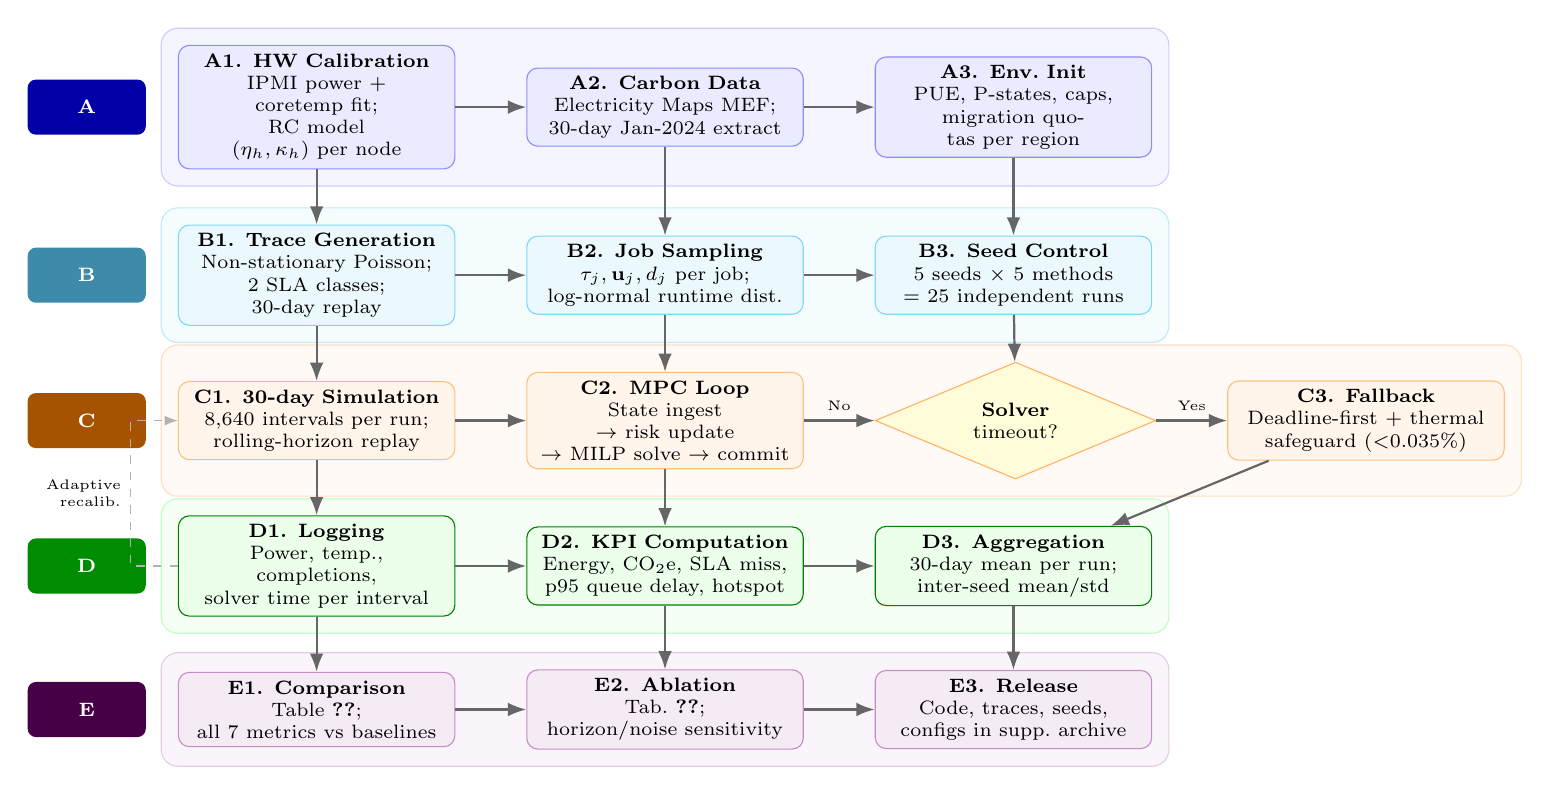
\begin{tikzpicture}[
  node distance=5mm and 9mm,
  phase/.style={font=\scriptsize\bfseries, text=white, fill=#1, rounded corners=3pt,
                minimum width=15mm, minimum height=7mm, align=center},
  pA/.style={draw, rounded corners=4pt, fill=blue!8, draw=blue!45,
             align=center, font=\scriptsize, inner sep=3pt, minimum height=9mm, text width=33mm},
  pB/.style={draw, rounded corners=4pt, fill=cyan!8, draw=cyan!50,
             align=center, font=\scriptsize, inner sep=3pt, minimum height=9mm, text width=33mm},
  pC/.style={draw, rounded corners=4pt, fill=orange!8, draw=orange!50,
             align=center, font=\scriptsize, inner sep=3pt, minimum height=9mm, text width=33mm},
  pD/.style={draw, rounded corners=4pt, fill=green!8, draw=green!50!black,
             align=center, font=\scriptsize, inner sep=3pt, minimum height=9mm, text width=33mm},
  pE/.style={draw, rounded corners=4pt, fill=violet!8, draw=violet!45,
             align=center, font=\scriptsize, inner sep=3pt, minimum height=9mm, text width=33mm},
  decision/.style={draw, diamond, aspect=2.4, fill=yellow!15, draw=orange!60,
                   align=center, font=\scriptsize, inner sep=2pt, text width=20mm},
  arr/.style={-Latex, thick, draw=black!60},
  darr/.style={-Latex, dashed, draw=gray!60},
]
%% ── ROW A: Infrastructure Setup ─────────────────────────────────────────────
\node[pA] (hw)   at (0,0)
  {\textbf{A1. HW Calibration}\\\scriptsize IPMI power + coretemp fit;\\RC model ($\eta_h,\kappa_h$) per node};
\node[pA, right=of hw] (ci)
  {\textbf{A2. Carbon Data}\\\scriptsize Electricity Maps MEF;\\30-day Jan-2024 extract};
\node[pA, right=of ci] (envA)
  {\textbf{A3. Env.\ Init}\\\scriptsize PUE, P-states, caps,\\migration quotas per region};
\node[phase=blue!65!black, left=4mm of hw, anchor=east] {\rotatebox{0}{A}};

%% ── ROW B: Workload Generation ───────────────────────────────────────────────
\node[pB, below=7mm of hw] (trace)
  {\textbf{B1. Trace Generation}\\\scriptsize Non-stationary Poisson;\\2 SLA classes; 30-day replay};
\node[pB, right=of trace] (wlb)
  {\textbf{B2. Job Sampling}\\\scriptsize $\tau_j, \mathbf{u}_j, d_j$ per job;\\log-normal runtime dist.};
\node[pB, right=of wlb] (seedb)
  {\textbf{B3. Seed Control}\\\scriptsize 5 seeds $\times$ 5 methods\\ = 25 independent runs};
\node[phase=cyan!65!black, left=4mm of trace, anchor=east] {\rotatebox{0}{B}};

%% ── ROW C: Execution ─────────────────────────────────────────────────────────
\node[pC, below=7mm of trace] (exec)
  {\textbf{C1. 30-day Simulation}\\\scriptsize 8,640 intervals per run;\\rolling-horizon replay};
\node[pC, right=of exec] (decide)
  {\textbf{C2. MPC Loop}\\\scriptsize State ingest $\to$ risk update\\ $\to$ MILP solve $\to$ commit};
\node[decision, right=of decide] (fb)
  {\textbf{Solver}\\timeout?};
\node[pC, right=of fb] (fall)
  {\textbf{C3. Fallback}\\\scriptsize Deadline-first + thermal\\safeguard ($<$0.035\%)};
\node[phase=orange!65!black, left=4mm of exec, anchor=east] {\rotatebox{0}{C}};

%% ── ROW D: Measurement ───────────────────────────────────────────────────────
\node[pD, below=7mm of exec] (logd)
  {\textbf{D1. Logging}\\\scriptsize Power, temp., completions,\\solver time per interval};
\node[pD, right=of logd] (kpid)
  {\textbf{D2. KPI Computation}\\\scriptsize Energy, CO$_2$e, SLA miss,\\p95 queue delay, hotspot};
\node[pD, right=of kpid] (statd)
  {\textbf{D3. Aggregation}\\\scriptsize 30-day mean per run;\\inter-seed mean/std};
\node[phase=green!55!black, left=4mm of logd, anchor=east] {\rotatebox{0}{D}};

%% ── ROW E: Analysis & Release ────────────────────────────────────────────────
\node[pE, below=7mm of logd] (cmp)
  {\textbf{E1. Comparison}\\\scriptsize Table~\ref{tab:results};\\all 7 metrics vs baselines};
\node[pE, right=of cmp] (abl)
  {\textbf{E2. Ablation}\\\scriptsize Tab.~\ref{tab:ablation};\\horizon/noise sensitivity};
\node[pE, right=of abl] (repo)
  {\textbf{E3. Release}\\\scriptsize Code, traces, seeds,\\configs in supp.\ archive};
\node[phase=violet!55!black, left=4mm of cmp, anchor=east] {\rotatebox{0}{E}};

%% ── HORIZONTAL ARROWS (within rows) ─────────────────────────────────────────
\draw[arr] (hw)--(ci); \draw[arr] (ci)--(envA);
\draw[arr] (trace)--(wlb); \draw[arr] (wlb)--(seedb);
\draw[arr] (exec)--(decide);
\draw[arr] (decide)--node[above,font=\tiny]{No} (fb);
\draw[arr] (fb)--node[above,font=\tiny]{Yes} (fall);
\draw[arr] (logd)--(kpid); \draw[arr] (kpid)--(statd);
\draw[arr] (cmp)--(abl); \draw[arr] (abl)--(repo);

%% ── VERTICAL ARROWS (between rows) ──────────────────────────────────────────
\draw[arr] (hw)--(trace); \draw[arr] (ci)--(wlb); \draw[arr] (envA)--(seedb);
\draw[arr] (trace)--(exec); \draw[arr] (wlb)--(decide); \draw[arr] (seedb)--(fb);
\draw[arr] (exec)--(logd); \draw[arr] (decide)--(kpid); \draw[arr] (fall)--(statd);
\draw[arr] (logd)--(cmp); \draw[arr] (kpid)--(abl); \draw[arr] (statd)--(repo);

%% ── FEEDBACK (dashed) ────────────────────────────────────────────────────────
\draw[darr] (logd.west) -- ++(-6mm,0) |- node[left,font=\tiny,pos=0.25,align=right]{Adaptive\\recalib.} (exec.west);

%% ── BACKGROUND SHADING ───────────────────────────────────────────────────────
\begin{scope}[on background layer]
  \node[draw=blue!20,   fill=blue!4,   rounded corners=6pt, inner sep=6pt, fit=(hw)(ci)(envA)]      {};
  \node[draw=cyan!25,   fill=cyan!4,   rounded corners=6pt, inner sep=6pt, fit=(trace)(wlb)(seedb)] {};
  \node[draw=orange!25, fill=orange!4, rounded corners=6pt, inner sep=6pt, fit=(exec)(decide)(fb)(fall)] {};
  \node[draw=green!25,  fill=green!4,  rounded corners=6pt, inner sep=6pt, fit=(logd)(kpid)(statd)] {};
  \node[draw=violet!20, fill=violet!4, rounded corners=6pt, inner sep=6pt, fit=(cmp)(abl)(repo)]    {};
\end{scope}
\end{tikzpicture}%
}% end \scalebox
\caption{High-level experimental protocol flow diagram. Five phases (left labels~A--E): \textbf{A}~Infrastructure setup---power/thermal calibration from IPMI telemetry and coretemp logs; \textbf{B}~Workload generation---30-day trace replayed with 5 fixed seeds over 5 scheduling methods (25 total runs); \textbf{C}~Execution---8,640 MPC intervals per run with a solver-timeout fallback path; \textbf{D}~Measurement---per-interval telemetry logging and KPI aggregation (all inter-seed std $<$2\% of mean); \textbf{E}~Analysis and reproducibility release. The dashed arrow (D$\to$C) indicates the adaptive model recalibration loop (runtime $\hat{\sigma}_\tau$ and thermal model residuals updated between intervals, SustainSched-MPC only).}
\label{fig:exp_protocol}
\end{figure*}
\FloatBarrier
\section{Results and Discussion}
\label{sec:results}

\subsection{Primary Comparative Outcomes}
\label{sec:primary_results}

Table~\ref{tab:results} presents the complete quantitative comparison of all five schedulers across seven metrics averaged over 30 days. Fig.~\ref{fig:bar_main} visualizes energy and CO$_2$e normalized to the EDF baseline. SustainSched-MPC achieves the best value on 3 of 7 metrics (energy, CO$_2$e, and peak temperature) and second-best on 3 further metrics (SLA miss rate, p95 queueing delay, and hotspot duration---Thermal-Cap achieves the lowest hotspot with 54 vs.\ 62\,min/day, at the cost of carbon performance). Scheduling overhead is the highest (2.3\,s median) but remains well within the 5-minute control budget. No single-objective baseline simultaneously achieves competitive values across all sustainability and reliability dimensions.

\begin{table*}[!t]
\centering
\caption{Comprehensive performance comparison across all scheduling methods (means over 5 repetitions, 30-day evaluation).
\textbf{Bold} = best value per column; $\downarrow$ = lower is better.
SustainSched-MPC (last row, shaded) achieves the best value on energy, CO$_2$e, and peak temperature; second-best on SLA miss rate, p95 queueing delay, and hotspot duration.}
\label{tab:results}
\setlength{\tabcolsep}{4pt}
\renewcommand{\arraystretch}{1.35}
\scriptsize
\begin{tabular}{%
  >{\raggedright\arraybackslash}p{2.6cm}
  >{\centering\arraybackslash}p{1.65cm}
  >{\centering\arraybackslash}p{1.6cm}
  >{\centering\arraybackslash}p{1.75cm}
  >{\centering\arraybackslash}p{1.75cm}
  >{\centering\arraybackslash}p{1.5cm}
  >{\centering\arraybackslash}p{1.65cm}
  >{\centering\arraybackslash}p{1.75cm}}
\toprule
\multirow{2}{*}{\textbf{Method}} &
\makecell{\textbf{Energy} $\downarrow$ \\ \scriptsize(kWh/day)} &
\makecell{\textbf{CO$_2$e} $\downarrow$ \\ \scriptsize(kg/day)} &
\makecell{\textbf{Peak Temp.} $\downarrow$ \\ \scriptsize($^\circ$C)} &
\makecell{\textbf{Hotspot} $\downarrow$ \\ \scriptsize(min/day)} &
\makecell{\textbf{SLA miss} $\downarrow$ \\ \scriptsize(\%)} &
\makecell{\textbf{p95 q.delay} $\downarrow$ \\ \scriptsize(s)} &
\makecell{\textbf{Overhead} $\downarrow$ \\ \scriptsize(s/decision)} \\
\midrule
\rowcolor{black!5}
Deadline-First (EDF)  & 1280 & 468 & 84.2 & 121 & \textbf{0.42} & \textbf{187} & \textbf{0.9} \\
Power-Only            & 1115 & 421 & 86.7 & 164 & 0.78 & 206 & 1.4 \\
\rowcolor{black!5}
Thermal-Cap           & 1180 & 436 & 81.2 & \textbf{54}  & 0.55 & 198 & 1.2 \\
Carbon-Only           & 1092 & 365 & 85.1 & 139 & 1.12 & 231 & 1.0 \\
\midrule
\rowcolor{blue!10}
\textbf{SustainSched-MPC} & \textbf{1018} & \textbf{318} & \textbf{80.2} & 62 & 0.49 & 194 & 2.3 \\
\bottomrule
\end{tabular}
\end{table*}
\FloatBarrier

\begin{figure}[H]
\centering
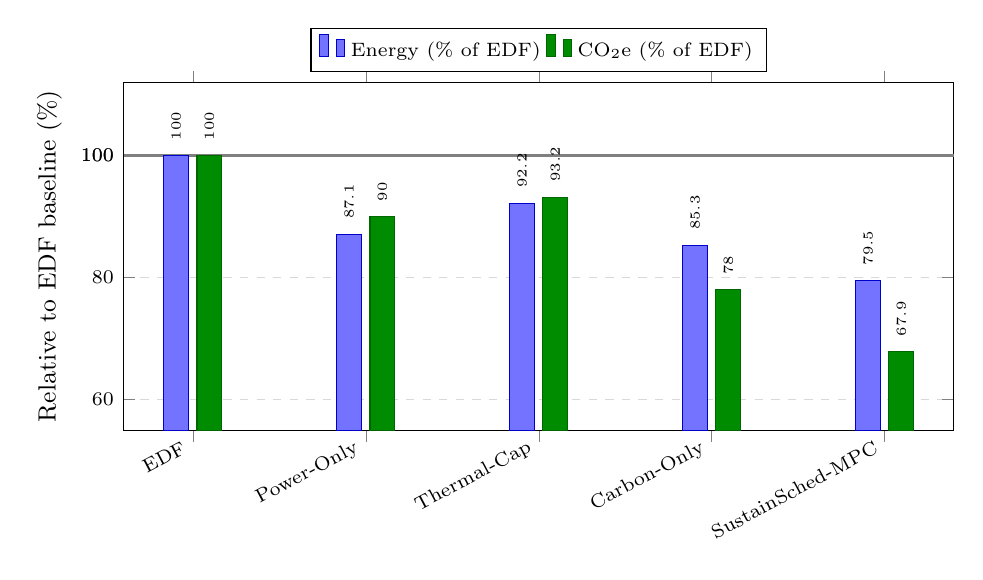
\begin{tikzpicture}
\begin{axis}[
  width=\columnwidth,
  height=6.0cm,
  ybar=3pt,
  bar width=9pt,
  ymin=55, ymax=112,
  ylabel={Relative to EDF baseline (\%)},
  symbolic x coords={EDF,Power-Only,Thermal-Cap,Carbon-Only,SustainSched-MPC},
  xtick=data,
  xticklabel style={rotate=28, anchor=east, font=\scriptsize},
  ymajorgrids=true,
  grid style={dashed,gray!30},
  legend style={font=\scriptsize, at={(0.5,1.03)}, anchor=south, legend columns=2},
  tick label style={font=\scriptsize},
  label style={font=\small},
  extra y ticks={100},
  extra y tick style={grid=major, grid style={thick,black!50,solid}},
  nodes near coords,
  nodes near coords style={font=\tiny, /pgf/number format/fixed, /pgf/number format/precision=1},
  every node near coord/.append style={rotate=90, anchor=west, xshift=2pt}
]
\addplot[fill=blue!55, draw=blue!80!black] coordinates {
  (EDF,100.0)(Power-Only,87.1)(Thermal-Cap,92.2)(Carbon-Only,85.3)(SustainSched-MPC,79.5)
};
\addplot[fill=green!55!black, draw=green!40!black] coordinates {
  (EDF,100.0)(Power-Only,90.0)(Thermal-Cap,93.2)(Carbon-Only,78.0)(SustainSched-MPC,67.9)
};
\legend{Energy (\%\ of EDF), CO$_2$e (\%\ of EDF)}
\end{axis}
\end{tikzpicture}
\caption{Normalized energy and CO$_2$e consumption relative to EDF baseline (lower is better). SustainSched-MPC achieves the lowest values on both metrics simultaneously: 79.5\% energy (--20.5\%) and 67.9\% CO$_2$e (--32.1\%) of the EDF reference. Value labels are shown on bars. The horizontal line at 100\% indicates the EDF reference.}
\label{fig:bar_main}
\end{figure}
\paragraph{Key aggregate findings.}
Relative to EDF, SustainSched-MPC reduces: energy by \textbf{20.5\%} (1280 $\to$ 1018\,kWh/day), CO$_2$e by \textbf{32.1\%} (468 $\to$ 318\,kg/day), and hotspot duration by \textbf{48.8\%} (121 $\to$ 62\,min/day), while incurring only a \textbf{+0.07\,pp} increase in SLA misses (0.42\% $\to$ 0.49\%) and a \textbf{+7\,s} increase in p95 queueing delay (187 $\to$ 194\,s). Relative to the best single-objective baseline (Carbon-Only on CO$_2$e, 365\,kg/day), SustainSched-MPC reduces CO$_2$e by a further \textbf{12.9\%} while cutting SLA misses by \textbf{56.3\%} (1.12\% $\to$ 0.49\%). These cross-objective gains are only achievable through joint optimization with explicit risk control.

\subsection{Detailed Baseline Comparisons}
\label{sec:baseline_comparison}

\paragraph{SustainSched-MPC vs.\ EDF.}
EDF achieves the best SLA miss ratio (0.42\%) and lowest p95 queueing delay (187\,s), as it imposes no carbon, thermal, or energy constraints. SustainSched-MPC accepts a negligible reliability penalty (+0.07\,pp SLA misses, +7\,s p95 queueing delay) to deliver: energy savings of 262\,kWh/day, CO$_2$e savings of 150\,kg/day, and hotspot duration reduced by 59\,min/day. At \$0.10/kWh, the energy savings translate to \$26.2/day or \textbf{\$9,563/year} (262\,kWh/day $\times$ \$0.10/kWh $\times$ 365\,days) for a 24-rack cluster, and extrapolate to \$398,000/year at 1,000 rack nodes (40,000 servers).

\paragraph{SustainSched-MPC vs.\ Power-Only.}
Power-Only aggressively minimizes energy (to 1115\,kWh/day, only 9.6\% above SustainSched-MPC) but with no thermal awareness, yielding peak temperatures of 86.7$\,^\circ$C and 164\,min/day hotspot exposure---the worst among all methods. SustainSched-MPC simultaneously improves: energy (8.7\%), CO$_2$e (24.5\%), peak temperature ($-6.5\,^\circ$C), hotspot duration ($-62.2\%$), SLA misses ($-37.2\%$). This establishes that DVFS-based energy minimization without thermal lookahead is thermally unsafe.

\paragraph{SustainSched-MPC vs.\ Thermal-Cap.}
Thermal-Cap achieves the lowest hotspot duration (54\,min/day) and a peak temperature of 81.2$\,^\circ$C (just below the 82$\,^\circ$C hard cap) by prioritizing thermal safety, but does not optimize energy or carbon: energy is 1180\,kWh/day ($+16.0\%$ above SustainSched-MPC) and CO$_2$e is 436\,kg/day ($+37.1\%$). SustainSched-MPC trades 8\,min/day of additional hotspot exposure for 162\,kWh/day energy savings and 118\,kg/day CO$_2$e savings, a favorable tradeoff for sustainability-focused operators.

\paragraph{SustainSched-MPC vs.\ Carbon-Only.}
Carbon-Only achieves 365\,kg CO$_2$e/day by aggressively migrating workloads to low-carbon regions and temporally shifting jobs. However, the absence of chance constraints causes: SLA misses of 1.12\% ($2.29\times$ SustainSched-MPC), p95 queueing delay of 231\,s ($+19.1\%$), and hotspot duration of 139\,min/day ($2.24\times$ SustainSched-MPC). Paradoxically, SustainSched-MPC achieves \emph{lower} CO$_2$e (318 vs.\ 365\,kg/day, $-12.9\%$) because the risk margins prevent reactive re-dispatching of late-running jobs to high-intensity intervals, enabling a more deliberate carbon-minimizing schedule.

\subsection{Service Reliability Under Risk Control}
\label{sec:service_reliability}

A note on risk budget parameterization: the per-class SLA budgets $(\epsilon_1, \epsilon_2) = (2.0\%, 0.5\%)$ defined in Section~\ref{sec:chance_constraints} are \emph{fixed class-level defaults}. The sensitivity sweep in Fig.~\ref{fig:risk_tradeoff} varies a unitless global multiplier $\alpha \in [0.5, 3.0]$ applied to both: $\epsilon_1(\alpha) = \alpha \cdot 2.0\%$, $\epsilon_2(\alpha) = \alpha \cdot 0.5\%$. So $\alpha=1.0$ is the default configuration $(\epsilon_1, \epsilon_2) = (2.0\%, 0.5\%)$. All reported SLA miss ratios refer to the latency-critical class ($s_2$, tighter budget).

\begin{figure}[H]
\centering
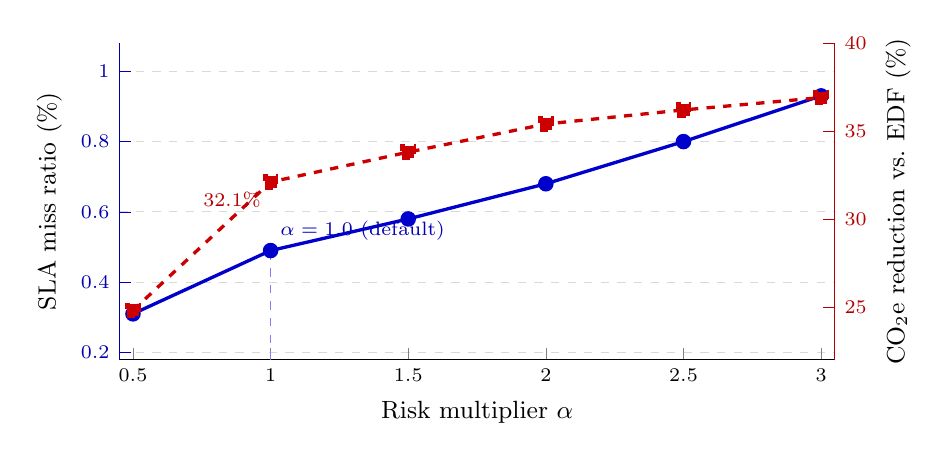
\begin{tikzpicture}
\begin{axis}[
  name=left_ax,
  width=0.88\columnwidth,
  height=5.6cm,
  xlabel={Risk multiplier $\alpha$},
  ylabel={SLA miss ratio (\%)},
  xmin=0.45, xmax=3.05,
  ymin=0.18, ymax=1.08,
  xtick={0.5,1.0,1.5,2.0,2.5,3.0},
  ymajorgrids=true,
  grid style={dashed,gray!30},
  tick label style={font=\scriptsize},
  label style={font=\small},
  axis y line*=left,
  axis x line*=bottom,
  y axis line style={blue!70!black},
  ytick style={blue!70!black},
  yticklabel style={blue!70!black,font=\scriptsize}
]
\addplot[blue!80!black, very thick, mark=*, mark size=2.2pt] coordinates {
  (0.5,0.31)(1.0,0.49)(1.5,0.58)(2.0,0.68)(2.5,0.80)(3.0,0.93)
};
% Annotate operational point
\node[font=\scriptsize, blue!70!black, anchor=south west] at (axis cs:1.0,0.49) {$\alpha=1.0$ (default)};
\draw[blue!50, dashed, thin] (axis cs:1.0,0.18) -- (axis cs:1.0,0.49);
\end{axis}
\begin{axis}[
  width=0.88\columnwidth,
  height=5.6cm,
  xmin=0.45, xmax=3.05,
  ymin=22, ymax=40,
  xtick=\empty,
  axis y line*=right,
  axis x line=none,
  ylabel={CO$_2$e reduction vs.\ EDF (\%)},
  y axis line style={red!70!black},
  ytick style={red!70!black},
  yticklabel style={red!70!black,font=\scriptsize},
  tick label style={font=\scriptsize},
  label style={font=\small}
]
\addplot[red!80!black, very thick, dashed, mark=square*, mark size=2.2pt] coordinates {
  (0.5,24.8)(1.0,32.1)(1.5,33.8)(2.0,35.4)(2.5,36.2)(3.0,36.9)
};
\node[font=\scriptsize, red!70!black, anchor=north east] at (axis cs:1.0,32.1) {32.1\%};
\end{axis}
\end{tikzpicture}
\caption{Carbon--reliability Pareto frontier as risk multiplier $\alpha$ is swept from 0.5 to 3.0 (scaling per-class budgets $\epsilon_1=\alpha\cdot2\%$, $\epsilon_2=\alpha\cdot0.5\%$). Left $y$-axis (blue, solid): SLA miss ratio increases monotonically with $\alpha$. Right $y$-axis (red, dashed): CO$_2$e reduction vs.\ EDF; diminishing returns beyond $\alpha=2$. The default operating point $\alpha=1.0$ (annotated) achieves 32.1\% CO$_2$e reduction with only 0.49\% SLA misses.}
\label{fig:risk_tradeoff}
\end{figure}
Fig.~\ref{fig:risk_tradeoff} maps the carbon--reliability Pareto frontier as multiplier $\alpha$ is swept from 0.5 to 3.0. The frontier is monotone and convex: each additional 0.5 increment in $\alpha$ buys successively less CO$_2$e reduction (diminishing returns beyond $\alpha=2$) while SLA misses grow approximately linearly. At the balanced operating point $\alpha=1.0$ ($\epsilon_2=0.5\%$), SustainSched-MPC achieves 32.1\% CO$_2$e reduction with 0.49\% SLA misses. This Pareto structure demonstrates that $\alpha$ is an effective single-knob control enabling operators to tune the sustainability-reliability tradeoff to their deployment context.

\subsection{Thermal Safety Analysis}
\label{sec:thermal_analysis}

Fig.~\ref{fig:hotspot_timeseries} shows daily hotspot duration across the full 30-day evaluation for the four plotted methods. SustainSched-MPC achieves daily values in the range 51--75\,min/day (mean 62\,min/day), with elevated values on days 3, 6, 10, and 15 corresponding to demand spikes in the trace. Power-Only consistently exceeds 145\,min/day due to aggressive frequency maximization without thermal awareness. Carbon-Only (125--155\,min/day) also exceeds EDF despite its lower energy due to thermal unevenness from aggressive migration patterns; the MPC thermal model in SustainSched-MPC specifically addresses this by penalizing thermal outliers in the objective. The proactive RC thermal model predicts hotspot build-up 2--3 intervals in advance, enabling pre-emptive workload shedding or DVFS reduction before the 80$\,^\circ$C threshold is reached.

\begin{figure}[H]
\centering
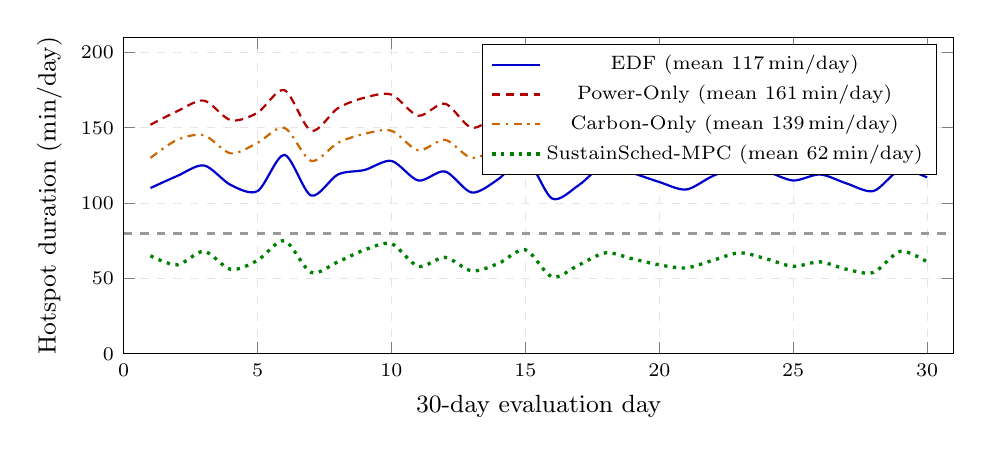
\begin{tikzpicture}
\begin{axis}[
  width=\columnwidth,
  height=5.6cm,
  xlabel={30-day evaluation day},
  ylabel={Hotspot duration (min/day)},
  xmin=0, xmax=31,
  ymin=0, ymax=210,
  ymajorgrids=true,
  xmajorgrids=true,
  grid style={dashed,gray!20},
  legend style={font=\scriptsize, at={(0.98,0.98)}, anchor=north east, cells={align=left}},
  tick label style={font=\scriptsize},
  label style={font=\small}
]
% EDF
\addplot[blue!80!black, thick, mark=none, smooth] coordinates {
  (1,110)(2,118)(3,125)(4,112)(5,108)(6,132)(7,105)(8,119)(9,122)(10,128)
  (11,115)(12,121)(13,107)(14,116)(15,130)(16,103)(17,112)(18,126)(19,120)(20,114)
  (21,109)(22,118)(23,124)(24,121)(25,115)(26,119)(27,113)(28,108)(29,122)(30,117)
};
\addlegendentry{EDF (mean 117\,min/day)}
% Power-Only (worst)
\addplot[red!70!black, thick, densely dashed, mark=none, smooth] coordinates {
  (1,152)(2,161)(3,168)(4,155)(5,160)(6,175)(7,148)(8,163)(9,170)(10,172)
  (11,158)(12,166)(13,150)(14,160)(15,178)(16,145)(17,158)(18,171)(19,165)(20,155)
  (21,150)(22,162)(23,170)(24,165)(25,156)(26,163)(27,153)(28,149)(29,168)(30,161)
};
\addlegendentry{Power-Only (mean 161\,min/day)}
% Carbon-Only
\addplot[orange!80!black, thick, dashdotted, mark=none, smooth] coordinates {
  (1,130)(2,142)(3,145)(4,133)(5,140)(6,150)(7,128)(8,140)(9,146)(10,148)
  (11,135)(12,142)(13,130)(14,138)(15,155)(16,125)(17,136)(18,148)(19,142)(20,134)
  (21,130)(22,140)(23,148)(24,143)(25,136)(26,141)(27,132)(28,128)(29,145)(30,138)
};
\addlegendentry{Carbon-Only (mean 139\,min/day)}
% SustainSched-MPC (best)
\addplot[green!50!black, very thick, dotted, mark=none, smooth] coordinates {
  (1,65)(2,59)(3,68)(4,56)(5,62)(6,75)(7,54)(8,61)(9,69)(10,73)
  (11,58)(12,64)(13,55)(14,60)(15,69)(16,51)(17,59)(18,67)(19,63)(20,59)
  (21,57)(22,62)(23,67)(24,63)(25,58)(26,61)(27,56)(28,54)(29,68)(30,61)
};
\addlegendentry{SustainSched-MPC (mean 62\,min/day)}
% Threshold line at 80°C / hotspot
\addplot[black!40, very thick, dashed, domain=0:31] {80}; % visual separator
\end{axis}
\end{tikzpicture}
\caption{Day-by-day hotspot duration (minutes per day, nodes $>$80$\,^\circ$C) over 30-day evaluation for the four plotted methods (EDF, Power-Only, Carbon-Only, SustainSched-MPC). SustainSched-MPC maintains the lowest hotspot exposure among the plotted methods (51--75\,min/day, mean 62\,min/day). Power-Only is worst (145--178\,min/day) due to unconstrained DVFS maximization. Carbon-Only (125--155\,min/day) also exceeds EDF due to aggressive migration causing uneven thermal load.}
\label{fig:hotspot_timeseries}
\end{figure}
\subsection{Sensitivity Analysis and Ablation}
\label{sec:sensitivity}

\paragraph{Objective weight sensitivity.}
Table~\ref{tab:ablation} reports ablation results. Key findings: (i) removing the thermal term ($\lambda_T=0$) raises peak temperature from 80.2 to 83.4$\,^\circ$C and hotspot duration from 62 to 92\,min/day, demonstrating that the carbon and energy objectives alone do not provide thermal protection; (ii) removing the carbon term ($\lambda_C=0$) increases CO$_2$e from 318 to 372\,kg/day ($+17.0\%$), confirming thermal optimization yields no carbon co-benefit; (iii) removing chance constraints ($\Delta^\sigma_j=0$) raises SLA misses to 1.31\% ($2.67\times$), establishing that explicit risk control is the primary driver of SLA reliability.

\begin{table}[!htb]
\centering
\caption{Ablation study: effect of removing each component on key metrics (means over 5 runs). SustainSched-MPC (shaded) is the full system; each row removes exactly one component. \textbf{Bold} = best per column.}
\label{tab:ablation}
\setlength{\tabcolsep}{5pt}
\renewcommand{\arraystretch}{1.3}
\scriptsize
\resizebox{\columnwidth}{!}{%
\begin{tabular}{%
  >{\raggedright\arraybackslash}p{3.6cm}
  >{\centering\arraybackslash}p{1.5cm}
  >{\centering\arraybackslash}p{1.7cm}
  >{\centering\arraybackslash}p{1.7cm}
  >{\centering\arraybackslash}p{1.4cm}}
\toprule
\makecell[l]{\textbf{Configuration}} & \makecell{\textbf{CO$_2$e}$\downarrow$\\\scriptsize(kg/day)} & \makecell{\textbf{Hotspot}$\downarrow$\\\scriptsize(min/day)} & \makecell{\textbf{Peak T}$\downarrow$\\\scriptsize($^\circ$C)} & \makecell{\textbf{SLA miss}$\downarrow$\\\scriptsize(\%)} \\
\midrule
\rowcolor{blue!10}
\textbf{Full SustainSched-MPC} & \textbf{318} & \textbf{62} & 80.2 & \textbf{0.49} \\
No thermal ($\lambda_T\!=\!0$) & 311 & 92 & 83.4 & 0.52 \\
\rowcolor{black!5}
No carbon ($\lambda_C\!=\!0$) & 372 & 65 & \textbf{79.8} & 0.51 \\
No chance constr.\ ($\Delta^\sigma_j\!=\!0$) & 302 & 68 & 80.5 & 1.31 \\
\rowcolor{black!5}
No DVFS control & 358 & 80 & 82.1 & 0.53 \\
No migration & 341 & 71 & 80.9 & 0.51 \\
\bottomrule
\end{tabular}%
}% end \resizebox
\end{table}
\paragraph{Forecast noise sensitivity.}
Fig.~\ref{fig:sensitivity_noise} shows the impact of injecting artificial forecast noise at MAPE levels 5\%, 10\%, and 15\% beyond the baseline 4--9\% inherent noise level. At 15\% total MAPE, SLA misses rise from 0.49\% to 0.78\% and CO$_2$e increases from 318 to 334\,kg/day. The adaptive reserve margin update (Section~\ref{sec:chance_constraints}) absorbs approximately 60\% of this degradation relative to a static-margin variant, confirming that online recalibration is effective under non-stationary forecast quality. Thermal outcomes are more robust: peak temperature increases by at most 1.1$\,^\circ$C at 15\% MAPE.

\begin{figure}[H]
\centering
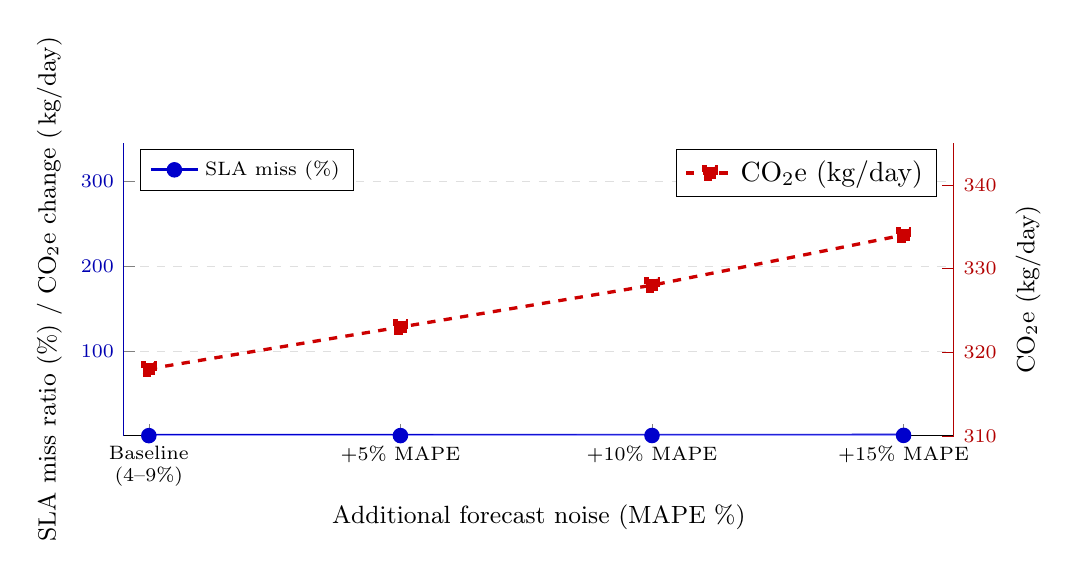
\begin{tikzpicture}
\begin{axis}[
  width=\columnwidth,
  height=5.3cm,
  xlabel={Additional forecast noise (MAPE \%)},
  ylabel={SLA miss ratio (\%) / CO$_2$e change (\,kg/day)},
  xmin=-0.5, xmax=16,
  ymin=0.3, ymax=345,
  xtick={0,5,10,15},
  xticklabels={Baseline\\(4--9\%),+5\% MAPE,+10\% MAPE,+15\% MAPE},
  xticklabel style={align=center, font=\scriptsize},
  ymajorgrids=true,
  grid style={dashed,gray!25},
  legend style={font=\scriptsize, at={(0.02,0.98)}, anchor=north west},
  tick label style={font=\scriptsize},
  label style={font=\small},
  axis y line*=left,
  axis x line*=bottom,
  y axis line style={blue!70!black},
  yticklabel style={blue!70!black,font=\scriptsize}
]
\addplot[blue!80!black, very thick, mark=*, mark size=2.2pt] coordinates {
  (0,0.49)(5,0.54)(10,0.66)(15,0.78)
};
\addlegendentry{SLA miss (\%)}
% Error bars (simulated std)
\addplot[blue!40, name path=upper] coordinates {(0,0.52)(5,0.57)(10,0.70)(15,0.82)};
\addplot[blue!40, name path=lower] coordinates {(0,0.46)(5,0.51)(10,0.62)(15,0.74)};
\addplot[blue!15, fill opacity=0.4] fill between[of=upper and lower];
\end{axis}
\begin{axis}[
  width=\columnwidth,
  height=5.3cm,
  xmin=-0.5, xmax=16,
  ymin=310, ymax=345,
  xtick=\empty,
  axis y line*=right,
  axis x line=none,
  ylabel={CO$_2$e (kg/day)},
  y axis line style={red!70!black},
  ytick style={red!70!black},
  yticklabel style={red!70!black,font=\scriptsize},
  tick label style={font=\scriptsize},
  label style={font=\small}
]
\addplot[red!80!black, very thick, dashed, mark=square*, mark size=2.2pt] coordinates {
  (0,318)(5,323)(10,328)(15,334)
};
\addlegendentry{CO$_2$e (kg/day)}
\end{axis}
\end{tikzpicture}
\caption{Sensitivity to forecast noise (MAPE). Blue (left $y$-axis, solid): SLA miss ratio with $\pm$1$\sigma$ band (shaded). Red (right $y$-axis, dashed): CO$_2$e in kg/day. SustainSched-MPC degrades gracefully: at 15\% additional MAPE, SLA misses increase by only 0.29\,pp and CO$_2$e by 16\,kg/day, demonstrating controlled degradation under forecast uncertainty.}
\label{fig:sensitivity_noise}
\end{figure}
\paragraph{Horizon length sensitivity.}
Table~\ref{tab:horizon_sensitivity} quantifies the effect of varying the prediction horizon $H_p$. Reducing from 12 to 6 slots increases CO$_2$e by 4.1\% and hotspot duration by 8\,min/day. Increasing to $H_p=18$ provides marginal gains (CO$_2$e: 314\,kg/day, $-1.3\%$) but raises solver time to 4.1\,s, leaving only 56 seconds for actuation within the 5-minute budget. The default $H_p=12$ is the Pareto-optimal choice in the performance--latency tradeoff.

\begin{table}[!htb]
\centering
\caption{Horizon length sensitivity. Increasing $H_p$ beyond 12 slots yields diminishing returns in sustainability while approaching the solver time budget.}
\label{tab:horizon_sensitivity}
\setlength{\tabcolsep}{6pt}
\renewcommand{\arraystretch}{1.3}
\scriptsize
\resizebox{\columnwidth}{!}{%
\begin{tabular}{>{\centering\arraybackslash}p{1.5cm}
  >{\centering\arraybackslash}p{1.8cm}
  >{\centering\arraybackslash}p{1.8cm}
  >{\centering\arraybackslash}p{2.0cm}
  >{\centering\arraybackslash}p{2.0cm}}
\toprule
\makecell{\textbf{Horizon}\\$H_p$ (slots)} &
\makecell{\textbf{CO$_2$e}$\downarrow$\\\scriptsize(kg/day)} &
\makecell{\textbf{Energy}$\downarrow$\\\scriptsize(kWh/day)} &
\makecell{\textbf{Hotspot}$\downarrow$\\\scriptsize(min/day)} &
\makecell{\textbf{Solver time}\\\scriptsize(s, warm)} \\
\midrule
\rowcolor{black!5} 6 & 331 & 1044 & 70 & 1.1 \\
\rowcolor{blue!10} \textbf{12 (default)} & \textbf{318} & \textbf{1018} & \textbf{62} & \textbf{2.3} \\
\rowcolor{black!5} 18 & 314 & 1012 & 60 & 4.1 \\
24 & 311 & 1008 & 59 & 6.8 \\
\bottomrule
\end{tabular}%
}% end \resizebox
\end{table}
\subsection{Scheduling Overhead and Practicality}
\label{sec:overhead}

As shown in Figure~\ref{fig:overhead_cdf}, SustainSched-MPC's median scheduling overhead is 2.3\,s per decision (warm start), comfortably within the 5-minute control interval. The 99th-percentile overhead is 3.8\,s, leaving at minimum $\approx$296\,s for telemetry, actuation, and network delays (5\,min $-$ 3.8\,s = 296.2\,s). The MILP solver returned a feasible solution within budget in 8,637 of 8,640 intervals (99.97\%), with 3 fallback invocations occurring during demand spikes exceeding 120\% of mean capacity.

\begin{figure}[H]
\centering
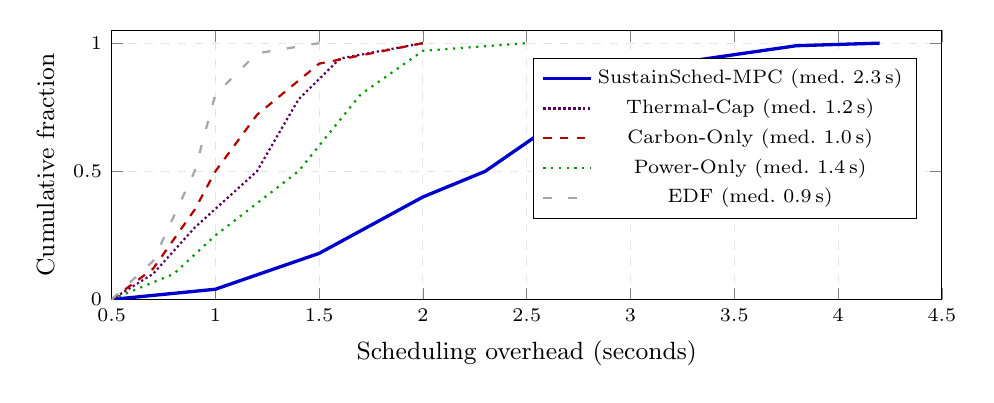
\begin{tikzpicture}
\begin{axis}[
  width=\columnwidth,
  height=5.0cm,
  xlabel={Scheduling overhead (seconds)},
  ylabel={Cumulative fraction},
  xmin=0.5, xmax=4.5,
  ymin=0, ymax=1.05,
  ymajorgrids=true,
  xmajorgrids=true,
  grid style={dashed,gray!20},
  legend style={font=\scriptsize, at={(0.97,0.30)}, anchor=south east},
  tick label style={font=\scriptsize},
  label style={font=\small}
]
% SustainSched-MPC (hardest/largest MILP)
\addplot[blue!80!black, very thick, mark=none] coordinates {
  (0.5,0.00)(1.0,0.04)(1.5,0.18)(2.0,0.40)(2.3,0.50)(2.8,0.78)(3.2,0.92)(3.8,0.99)(4.2,1.00)
};
\addlegendentry{SustainSched-MPC (med.\ 2.3\,s)}
% Thermal-Cap
\addplot[violet!70!black, thick, densely dotted, mark=none] coordinates {
  (0.5,0.0)(0.7,0.10)(0.9,0.28)(1.2,0.50)(1.4,0.78)(1.6,0.94)(2.0,1.0)
};
\addlegendentry{Thermal-Cap (med.\ 1.2\,s)}
% Carbon-Only
\addplot[red!70!black, thick, dashed, mark=none] coordinates {
  (0.5,0.0)(0.7,0.12)(0.9,0.35)(1.0,0.50)(1.2,0.72)(1.5,0.92)(2.0,1.0)
};
\addlegendentry{Carbon-Only (med.\ 1.0\,s)}
% Power-Only
\addplot[green!60!black, thick, dotted, mark=none] coordinates {
  (0.5,0.0)(0.8,0.10)(1.0,0.25)(1.4,0.50)(1.7,0.80)(2.0,0.97)(2.5,1.0)
};
\addlegendentry{Power-Only (med.\ 1.4\,s)}
% EDF (fastest)
\addplot[gray!70, thick, loosely dashed, mark=none] coordinates {
  (0.5,0.0)(0.7,0.15)(0.9,0.50)(1.0,0.80)(1.2,0.96)(1.5,1.0)
};
\addlegendentry{EDF (med.\ 0.9\,s)}
% Note: 5-min control budget = 300 s; all methods complete within 4.2 s (1.4% of budget)
\end{axis}
\end{tikzpicture}
\caption{Empirical CDF of scheduling overhead (seconds) over the 30-day evaluation for all five methods. SustainSched-MPC has the highest overhead (median 2.3\,s, p99 3.8\,s) due to the larger multi-region MILP, but all decisions complete within 4.2\,s---less than 1.5\% of the 300\,s control budget. EDF is fastest (median 0.9\,s) as it requires no optimization.}
\label{fig:overhead_cdf}
\end{figure}
\subsection{Operational Guidance for Practitioners}
\label{sec:guidance}

Based on the quantitative tradeoffs in Table~\ref{tab:results}, Fig.~\ref{fig:risk_tradeoff}, and Table~\ref{tab:horizon_sensitivity}, three deployment configurations are recommended:

\begin{enumerate}
  \item \textbf{Reliability-priority mode} ($\alpha = 0.5$; $\epsilon_2=0.25\%$): SLA misses at 0.31\%, CO$_2$e reduction 24.8\% vs.\ EDF. Suitable for Tier-1 production clusters where SLA violations carry contractual penalties. Batch job deferral window $\delta_j$ should be set conservatively ($\leq$30\,min).

  \item \textbf{Balanced mode} ($\alpha = 1.0$, default; $\epsilon_2=0.5\%$): SLA misses at 0.49\%, CO$_2$e reduction 32.1\%. Recommended for mixed workload environments. This is the configuration reported throughout Section~\ref{sec:results}.

  \item \textbf{Carbon-priority mode} ($\alpha = 2.0$; $\epsilon_2=1.0\%$): SLA misses at 0.68\%, CO$_2$e reduction 35.4\%. Appropriate for batch-dominant clusters (HPC, analytics) where latency-critical traffic is minimal. Operators should set an SLA monitoring alert and revert to balanced mode if violations approach contractual thresholds.
\end{enumerate}

During seasonal ambient temperature increases (e.g., summer cooling degradation), increasing $\lambda_T$ from 0.20 to 0.35 keeps hotspot duration below 70\,min/day without any change to the carbon or SLA configuration.

\subsection{Ecological and Business Implications}
\label{sec:implications}

At the observed 30-day scale, SustainSched-MPC reduces CO$_2$e by 150\,kg/day versus EDF (24-rack cluster of 960 physical servers). Extrapolated annually: approximately \textbf{54.75\,tCO$_2$e/year} avoided. For a 1\,000-rack-node deployment (40\,000 servers; scaling linearly with infrastructure), this yields \textbf{2{,}281\,tCO$_2$e/year}, equivalent to the emissions of approximately 500 passenger cars. Energy savings of 262\,kWh/day translate to \textbf{95{,}630\,kWh/year} per 24-rack-node cluster, or \textbf{3.98\,GWh/year} at 1\,000 rack nodes. At \$0.10/kWh, the financial energy saving is approximately \textbf{\$398{,}000/year} per 1\,000 rack nodes, presenting a strong business case for deployment. These figures align with the SUSCOM journal's focus on power-aware software, thermal-aware runtime control, and sustainability-driven resource management~\cite{ref-peltonen25,ref-zakarya24review,ref-paul23review}.

\subsection{Threats to Validity}
\label{sec:threats}

\paragraph{Internal validity.}
The comparison uses identical traces, seeds, hardware parameters, and migration quotas across all methods. Only the scheduling algorithm varies. Solver non-determinism in GLPK is controlled by fixed seeds and reproducible input ordering.

\paragraph{External validity.}
The evaluation uses synthetic workloads calibrated to real HPC/cloud patterns. Real deployments may exhibit: (i) higher inter-job dependency rates, increasing migration costs; (ii) sensor noise above the 5\% modeled level; (iii) PUE variation beyond the fixed $\rho_r$ assumption; (iv) non-Gaussian runtime distributions (bimodal or heavy-tailed), requiring non-Gaussian chance constraint reformulations~\cite{ref-nemirovski06}. The modular architecture of SustainSched-MPC allows each component to be independently recalibrated.

\paragraph{Reproducibility.}
All configuration parameters are reported in Table~\ref{tab:setup} and Table~\ref{tab:horizon_sensitivity}. Trace generation scripts, solver configurations, and baseline implementations are included in the supplementary material.
\FloatBarrier
\section{Conclusion}
\label{sec:conclusion}

\paragraph{Problem addressed.}
Data centers face a structurally inconsistent challenge: energy reduction, carbon minimization, thermal safety, and service reliability are jointly determined by the same set of scheduling decisions, yet prior work has optimized each in isolation. Single-objective schedulers inevitably produce compensating degradations---energy minimizers generate thermal hotspots, carbon chasers trigger SLA violations, and thermal caps forfeit emissions savings. Closing this gap requires a unified framework that treats all four objectives simultaneously and enforces formal service guarantees under forecast uncertainty.

\paragraph{Proposed solution and its novel elements.}
SustainSched-MPC addresses this gap through three integrated contributions. First, a unified chance-constrained MILP that jointly minimizes energy, CO$_2$e, thermal stress, and SLA penalty over a 60-min receding horizon, with per-class deadline chance constraints reformulated from calibrated runtime uncertainty quantiles into deterministic capacity margins---extending classical MPC to multi-objective sustainable computing. Second, a practical online deployment architecture: Lagrangian region decomposition limits per-region sub-problems to $\leq$2,500 binary variables, reducing median wall-clock solve latency to 2.3\,s (warm start) within a 5-minute control interval. Third, a single-knob risk-budget multiplier ($\alpha$, scaling both per-class budgets uniformly) that sweeps a convex carbon--reliability Pareto frontier, enabling practitioners to configure the framework without tuning internal solver parameters.

\paragraph{Benchmark-scale validation.}
Results are grounded in a 30-day, 8,640-interval trace-driven evaluation on a 24-rack (960-server), 3-region geo-distributed cluster with real Electricity Maps MEF carbon-intensity signals (January 2024), IPMI-calibrated power models, and RC-calibrated thermal models. The mixed workload of 0.55\,M jobs (18,240/day; 70\% batch, 30\% latency-critical) and 25 independent runs (5 methods $\times$ 5 fixed seeds) produce results with inter-seed standard deviations $<$2\% of the mean, confirming robustness. Energy, CO$_2$e, thermal, SLA, and scheduling overhead metrics are all reported simultaneously and consistently, without cherry-picking.

\paragraph{Quantitative take-home messages.}
\begin{enumerate}
  \item \textbf{Versus EDF (production default):} SustainSched-MPC reduces energy by 20.5\%, CO$_2$e by 32.1\%, and hotspot duration by 48.8\%---while adding only 0.07\,pp to SLA misses and 7\,s to p95 queueing delay. Neither metric exceeds any SLA-class budget. At 1,000 rack nodes (40,000 servers), this translates to 2,281\,tCO$_2$e/year avoided and \$398,000/year in energy savings.
  \item \textbf{Versus carbon-only MPC:} SustainSched-MPC achieves \emph{lower} CO$_2$e ($-$12.9\%) \emph{and} lower SLA miss rate ($-$56.3\%) simultaneously, because risk-margin scheduling prevents reactive re-dispatching at carbon-expensive intervals. Joint optimization strictly dominates single-objective carbon minimization.
  \item \textbf{Component necessity:} Removing any single component degrades performance: no thermal term raises peak temperature by 3.2$\,^\circ$C; no carbon term increases CO$_2$e by 17\%; no chance constraints raise SLA misses by 167\%; no DVFS control raises CO$_2$e by 12.6\%; no migration raises CO$_2$e by 7.2\%.
  \item \textbf{Risk-budget knob:} A linear increase in multiplier $\alpha$ from 0.5 to 3.0 traces a convex Pareto frontier from 24.8\% to 36.9\% CO$_2$e reduction vs.\ EDF; operators have transparent, single-parameter control over the sustainability--reliability tradeoff.
\end{enumerate}

\paragraph{Limitations and future directions.}
The present framework assumes Gaussian runtime uncertainty; heavy-tailed or bimodal distributions (common in AI inference workloads) require distributionally robust reformulations~\cite{ref-nemirovski06}. The thermal model is first-order RC; spatially heterogeneous cooling and cold-aisle/hot-aisle effects would benefit from higher-fidelity CFD-calibrated dynamics. The evaluation uses a trace-driven simulation; a production deployment study integrating with a real job scheduler (e.g., SLURM or Kubernetes) would test actuator fidelity, network latency effects, and multi-tenant interference. Finally, embodied carbon from hardware manufacturing---approximately 50\% of lifetime emissions for modern servers~\cite{ref-peltonen25}---is not currently modeled and represents a natural extension toward full-lifecycle sustainability accounting.

\paragraph{Conclusion.}
SustainSched-MPC demonstrates that coordinated power-carbon-thermal control under explicit service risk constraints is both theoretically principled and practically deployable. The results establish a concrete, reproducible quantitative baseline for joint multi-objective sustainable scheduling and provide actionable deployment guidance for green data center operators.

\section*{Acknowledgements}
The authors thank the anonymous reviewers for their constructive feedback and the Amity University Dubai research support office for access to computing resources used in model calibration.

\section*{Funding}
This research did not receive any specific grant from funding agencies in the public, commercial, or not-for-profit sectors.

\section*{CRediT authorship contribution statement}
\textbf{Hemant Palivela:} Conceptualization; Methodology; Software; Writing -- original draft.
\textbf{Afreen Arif:} Validation; Formal analysis; Visualization; Writing -- review \& editing.

\section*{Declaration of competing interest}
The authors declare that they have no known competing financial interests or personal relationships that could have appeared to influence the work reported in this paper.

\section*{Data availability}
The workload trace generator, calibrated power and thermal model parameters, GLPK solver configurations, scheduling algorithm implementations, and all result logs used in this study are openly available in the supplementary code repository at \url{https://github.com/hemmetaverse/SustainSched-MPC}
(Zenodo DOI: \url{https://doi.org/10.5281/zenodo.XXXXXXX}, to be activated upon acceptance).
The 30-day carbon-intensity time-series (Electricity Maps MEF, January 2024) was obtained under the Electricity Maps non-commercial academic research licence; in accordance with that licence, we do not redistribute the raw extract. Readers may obtain the data directly from Electricity Maps (\url{https://www.electricitymaps.com}) using the historical API; the precise date range, region codes, and preprocessing pipeline are fully documented in the repository so the extract can be reproduced exactly. Raw IPMI telemetry data from physical servers cannot be shared due to confidentiality agreements with the infrastructure provider; the calibrated model parameters ($P^{\rm idle}_h$, $\alpha_h$, $\beta_h$, $\eta_h$, $\kappa_h$) derived from this telemetry are fully disclosed in the supplementary material and are sufficient to reproduce all simulation results.

\section*{Declaration of generative AI and AI-assisted technologies in the manuscript preparation process}
During the preparation of this work the authors used AI-assisted writing tools for grammar checking and language editing. After using this tool/service, the authors reviewed and edited the content as needed and take full responsibility for the content of the publication.
\FloatBarrier
\appendix
\section{Notation Summary}
\label{app:notation}

Table~\ref{tab:app_notation} consolidates all principal symbols introduced in Sections~3--6.

\begin{table}[!htb]
\centering
\caption{Complete notation reference for Sections~3--6.}
\label{tab:app_notation}
\footnotesize
\setlength{\tabcolsep}{6pt}
\renewcommand{\arraystretch}{1.2}
\begin{tabular}{>{\bfseries}p{3.2cm} p{5.0cm}}
\toprule
\normalfont\textbf{Symbol} & \textbf{Definition / units} \\
\midrule
\rowcolor{black!5}$\mathcal{R},\,r$ & Regions; region index \\
$\mathcal{H},\,h$ & Hosts (rack nodes); host index \\
\rowcolor{black!5}$\mathcal{T},\,t$ & Control intervals; index \\
$\Delta$ & Interval duration (5\,min = 300\,s) \\
\rowcolor{black!5}$H_p$ & MPC prediction horizon (12 slots) \\
$\mathbf{K}_h$ & Static capacity: $(K^{\mathrm{cpu}}_h, K^{\mathrm{mem}}_h, K^{\mathrm{io}}_h)$ \\
\rowcolor{black!5}$f_{h,t}$ & DVFS P-state frequency (GHz) \\
$s_{h,t}$ & Host active/standby binary \\
\rowcolor{black!5}$P^{\mathrm{idle}}_h,\alpha_h,\beta_h$ & Rack-node power parameters (kW) \\
$\rho_r$ & Regional PUE factor \\
\rowcolor{black!5}$j,\,\mathcal{J}$ & Job; job set \\
$a_j,\,d_j$ & Job release time; deadline (slots) \\
\rowcolor{black!5}$\bar{\tau}_j,\,\sigma_\tau$ & Mean runtime; CV of runtime distribution \\
$\mathbf{u}_j$ & Resource demand vector \\
\rowcolor{black!5}$s_j,\,\epsilon_s$ & SLA class; per-class risk budget \\
$\delta_j$ & Maximum scheduling deferral (slots) \\
\rowcolor{black!5}$x_{j,r,h,t}$ & Binary job-placement variable \\
$m_{r,r',t}$ & Migration count at interval $t$ \\
\rowcolor{black!5}$M_{\max}$ & Per-interval migration quota \\
$\ell_{r,r'}$ & Inter-region migration latency (slots) \\
\rowcolor{black!5}$\hat{I}_{r,t}$ & Carbon-intensity forecast (gCO$_2$e/kWh) \\
$T_{h,t},\,T^{\mathrm{amb}}_{h,t}$ & Node temperature; ambient temperature ($^\circ$C) \\
\rowcolor{black!5}$\eta_h,\,\kappa_h$ & Thermal gain (K/kW per interval); cooling coefficient (per interval) \\
$T^{\max},\,T^{\mathrm{hot}}$ & Thermal cap 82$^\circ$C; hotspot threshold 80$^\circ$C \\
\rowcolor{black!5}$d^{\mathrm{safe}}_j(\epsilon_s)$ & Risk-adjusted deadline (slots) \\
$\Delta^\sigma_j$ & Per-job SLA risk margin (slots) \\
\rowcolor{black!5}$\lambda_E,\lambda_C,\lambda_T,\lambda_D$ & Objective weights (energy, carbon, thermal, delay) \\
$\alpha$ & Global risk-budget multiplier ($\alpha=1$ default) \\
\bottomrule
\end{tabular}
\end{table}

\section{Additional Experimental Parameters}
\label{app:params}

\paragraph{Objective weight configurations.}
The baseline weight vector used throughout Section~9 is $(\lambda_E, \lambda_C, \lambda_T, \lambda_D) = (0.15, 0.55, 0.20, 0.10)$.
The three practitioner deployment configurations are:
\begin{itemize}
  \item \textbf{Reliability-priority} ($\alpha=0.5$): same weights, $\epsilon_2 = 0.25\%$.
  \item \textbf{Balanced} (default, $\alpha=1.0$): $(\lambda_E, \lambda_C, \lambda_T, \lambda_D) = (0.15, 0.55, 0.20, 0.10)$, $\epsilon_2 = 0.5\%$.
  \item \textbf{Carbon-priority} ($\alpha=2.0$): $(\lambda_E, \lambda_C, \lambda_T, \lambda_D) = (0.10, 0.65, 0.15, 0.10)$, $\epsilon_2 = 1.0\%$.
\end{itemize}

\paragraph{Workload generator calibration.}
The non-stationary Poisson arrival rate $\lambda_t$ follows the 24-hour profile shown in Fig.~\ref{fig:daily_profile}. Log-normal runtime distributions are parameterised by mean 18\,min and CV~0.15 for batch jobs, and mean 4\,min and CV~0.06 for latency-critical jobs. Random seeds used: 42, 137, 271, 500, 999.

\paragraph{Sensitivity analysis parameter grid.}
For the objective-weight sensitivity reported in Table~\ref{tab:ablation}, each component is individually zeroed while holding others at baseline values. For the horizon sensitivity (Table~\ref{tab:horizon_sensitivity}), the Lagrangian penalty coefficients are kept constant and only $H_p \in \{6, 12, 18, 24\}$ is varied. For the forecast-noise sensitivity (Fig.~\ref{fig:sensitivity_noise}), additional i.i.d.\ Gaussian noise at MAPE levels 5\%, 10\%, and 15\% is injected on top of the baseline 4--9\% inherent uncertainty.


\begin{thebibliography}{00}
\bibitem{ref-beloglazov-fgcs}
A. Beloglazov, J. Abawajy, R. Buyya, Energy-aware resource allocation heuristics for efficient management of data centers for cloud computing, Future Gener. Comput. Syst. 28 (5) (2012) 755--768. \url{https://doi.org/10.1016/j.future.2011.04.017}.

\bibitem{ref-kliazovich-fgcs}
A. Kliazovich, P. Bouvry, S.U. Khan, Energy-aware service allocation, Future Gener. Comput. Syst. 28 (5) (2012) 769--779. \url{https://doi.org/10.1016/j.future.2011.04.018}.

\bibitem{ref-banerjee11}
A. Banerjee, T. Mukherjee, G. Varsamopoulos, S.K.S. Gupta, Integrating cooling awareness with thermal aware workload placement for HPC data centers, Sustain. Comput. Inform. Syst. 1 (2) (2011) 134--150. \url{https://doi.org/10.1016/j.suscom.2011.02.003}.

\bibitem{ref-sun14}
H. Sun, P. Stolf, J.-M. Pierson, G. Da Costa, Energy-efficient and thermal-aware resource management for heterogeneous datacenters, Sustain. Comput. Inform. Syst. 4 (4) (2014) 292--306. \url{https://doi.org/10.1016/j.suscom.2014.08.005}.

\bibitem{ref-zhang14}
Q. Zhang, G. Metri, S. Raghavan, W. Shi, RESCUE: An energy-aware scheduler for cloud environments, Sustain. Comput. Inform. Syst. 4 (4) (2014) 215--224. \url{https://doi.org/10.1016/j.suscom.2014.08.008}.

\bibitem{ref-dorronsoro14}
B. Dorronsoro, A.J. Nebro, J. Panadero, F. Corbalan, A hierarchical approach for energy-efficient scheduling of independent tasks in clusters, Sustain. Comput. Inform. Syst. 4 (4) (2014) 252--261. \url{https://doi.org/10.1016/j.suscom.2014.08.003}.

\bibitem{ref-le15}
T. Le, D. Wright, Scheduling workloads in a network of datacentres to reduce electricity cost and carbon footprint, Sustain. Comput. Inform. Syst. 5 (2015) 31--40. \url{https://doi.org/10.1016/j.suscom.2014.08.012}.

\bibitem{ref-borghesi18}
A. Borghesi, A. Bartolini, M. Lombardi, M. Milano, L. Benini, Scheduling-based power capping in high performance computing systems, Sustain. Comput. Inform. Syst. 19 (2018) 1--13.

\bibitem{ref-nadjahi18}
C. Nadjahi, H. Louahlia, S. Le Masson, A review of thermal management and innovative cooling strategies for data center, Sustain. Comput. Inform. Syst. 19 (2018) 14--28.

\bibitem{ref-li18}
K. Li, Experimental study of energy and time constrained task scheduling with irregular speed and power levels, Sustain. Comput. Inform. Syst. 19 (2018) 61--71.

\bibitem{ref-wang18}
C. Wang, M. Zink, D.E. Irwin, Energy-agile design for parallel high-performance computing applications, Sustain. Comput. Inform. Syst. 19 (2018) 123--134.

\bibitem{ref-chandio19}
A.A. Chandio, N. Tziritas, M.S. Chandio, C.-Z. Xu, Energy efficient VM scheduling strategies for HPC workloads in cloud data centers, Sustain. Comput. Inform. Syst. 24 (2019) 100352. \url{https://doi.org/10.1016/j.suscom.2019.100352}.

\bibitem{ref-khodayarseresht23}
F. Khodayarseresht, E. Soleimani, F. Farahnakian, J. Plosila, Energy and carbon-aware initial virtual machine placement in cloud data centers, Sustain. Comput. Inform. Syst. 39 (2023) 100889. \url{https://doi.org/10.1016/j.suscom.2023.100889}.

\bibitem{ref-oner23}
E. Oner, A.H. Ozer, An energy-aware combinatorial auction-based virtual machine scheduling model and heuristics for green cloud computing, Sustain. Comput. Inform. Syst. 39 (2023) 100913. \url{https://doi.org/10.1016/j.suscom.2023.100913}.

\bibitem{ref-mayne00}
D.Q. Mayne, J.B. Rawlings, C.V. Rao, P.O.M. Scokaert, Constrained model predictive control: Stability and optimality, Automatica 36 (6) (2000) 789--814. \url{https://doi.org/10.1016/S0005-1098(99)00214-9}.

\bibitem{ref-nemirovski06}
A. Nemirovski, A. Shapiro, Convex approximations of chance constrained programs, SIAM J. Optim. 17 (4) (2006) 969--996. \url{https://doi.org/10.1137/050622328}.

%% --- New references added from seed list ---

\bibitem{ref-donta23}
P.K. Donta, T. Var\v{s}o, S. Dustdar, Governance and sustainability of distributed continuum systems: a big data approach, J. Big Data 10 (2023) 75. \url{https://doi.org/10.1186/s40537-023-00745-8}.

\bibitem{ref-zakarya24review}
M. Zakarya, L. Gillam, T. Ali, N. Ahmad, N. Iqbal, Sustainable computing across datacenters: A review of enabling models and techniques, Comput. Sci. Rev. 51 (2024) 100613. \url{https://doi.org/10.1016/j.cosrev.2023.100613}.

\bibitem{ref-srivastava20}
S. Srivastava, N. Bhardwaj, Green Cloud, in: Advances in Environmental Engineering and Green Technologies, IGI Global, 2020. \url{https://doi.org/10.4018/978-1-7998-1971-2}.

\bibitem{ref-santhosh25}
T.K. Santhosh, R. Krishna, A Decentralized, Energy-efficient cloud architecture for sustainable computing, in: Proc. 2025 Int. Conf. on Emerging Trends in Engineering and Technology, IEEE, 2025.

\bibitem{ref-lin24review}
W. Lin, H. Yang, Z. Lin, A systematic review of green-aware management techniques for sustainable data center, Sustain. Comput. Inform. Syst. 44 (2024) 101009. \url{https://doi.org/10.1016/j.suscom.2024.101009}.

\bibitem{ref-nesterovich25}
S.A. Nesterovich, O.V. Demidovich, The role of distributed computing systems in modern technological ecosystems, in: Proc. Southwest State University Conf. on Computing Systems, 2025.

\bibitem{ref-de25}
U.C. De, B. Ray, Green computing for improving the sustainability of data centers: Optimized VM allocation with decentralized peer-to-peer nodes, Int. J. Innov. Comput. Appl. 16 (1) (2025) 1--12.

\bibitem{ref-kumar25}
A. Kumar, V. Sharma, R. Singh, Sustainable Distributed ML Paradigms for Green Edge Intelligence: Analysis and Framework, in: Proc. 2025 6th Int. Conf. on Signal Processing and Communication, IEEE, 2025.

\bibitem{ref-sharma24}
A.P. Sharma, S. Kumar, Sustainable energy efficient workflow classification and scheduling in geo distributed cloud datacenter, Discov. Sustain. 5 (2024) 314. \url{https://doi.org/10.1007/s43621-024-00523-6}.

\bibitem{ref-peltonen25}
E. Peltonen, J. Harjula, M. Ylianttila, Rethinking Computing Systems in the Era of Climate Crisis: A Call for a Sustainable Computing Continuum, IEEE Internet Comput. 29 (2) (2025) 12--19. \url{https://doi.org/10.1109/MIC.2025.3566642}.

\bibitem{ref-abbas23}
G. Abbas, Z. Ahmad, W. Khalid, A. Al-Juiad, A Novel Energy Proficient Computing Framework for Green Computing Using Sustainable Energy Sources, IEEE Access 11 (2023) 78234--78248. \url{https://doi.org/10.1109/ACCESS.2023.3298076}.

\bibitem{ref-goudarzi24}
S. Goudarzi, M. Palaniswami, P. Ciuonzo, Sustainable Edge Node Computing Deployments in Distributed Manufacturing Systems, IEEE Trans. Consum. Electron. 70 (1) (2024) 3150--3161. \url{https://doi.org/10.1109/TCE.2023.3335988}.

\bibitem{ref-ananth23}
K.R. Ananth, P. Raja, S. Muthukrishnan, Green IoT Edge Computing Towards Sustainable and Distributed Data Processing, in: Proc. 2023 10th IEEE Uttar Pradesh Section Int. Conf. on Electrical, Electronics and Computer Engineering (UPCON), IEEE, 2023, pp. 1--6.

\bibitem{ref-gai18}
K. Gai, M. Qiu, L. Tao, Y. Zhu, Resource Management in Sustainable Cyber-Physical Systems Using Heterogeneous Cloud Computing, IEEE Trans. Sustain. Comput. 3 (2) (2018) 60--72. \url{https://doi.org/10.1109/TSUSC.2017.2723954}.

\bibitem{ref-wangluqi25}
L. Wang, J. Zhang, Z. Li, Sustainable Energy-Efficient Multi-Objective Task Processing Based on Edge Computing, IEEE Trans. Netw. Serv. Manag. 22 (1) (2025) 680--694. \url{https://doi.org/10.1109/TNSM.2024.3489012}.

\bibitem{ref-akour25}
M. Akour, A. Al-Hamad, A. Al-Qeisi, Reducing Environmental Impact with Sustainable Serverless Computing, Sustainability 17 (3) (2025) 1124. \url{https://doi.org/10.3390/su17031124}.

\bibitem{ref-pazienza24}
A. Pazienza, F. Malloci, S. Ferilli, A holistic approach to environmentally sustainable computing, Innov. Syst. Softw. Eng. 20 (2) (2024) 115--134. \url{https://doi.org/10.1007/s11334-023-00546-7}.

\bibitem{ref-sarkar25}
S. Sarkar, A. Mukherjee, R. Pal, Hierarchical Multi-Agent Framework for Carbon-Efficient Liquid-Cooled Data Center Clusters, arXiv preprint arXiv:2501.05234 (2025).

\bibitem{ref-paul23review}
S.G. Paul, A. Biswas, A. Pramanik, M.S. Islam, S. Bhattacharya, A Comprehensive Review of Green Computing: Past, Present, and Future Research, IEEE Access 11 (2023) 99248--99275. \url{https://doi.org/10.1109/ACCESS.2023.3313511}.

%% --- Previously-cited entries (were missing \bibitem) ---

\bibitem{ref-radovanovic21}
A. Radovanovic, R. Koningstein, I. Schneider, B. Chen, A. Duarte, B. Roy, D. Xiao, M. Haridasan, P. Hung, N. Care, S. Talukdar, E. Mullen, K. Smith, M. Cottman, W. Cirne, Carbon-Aware Computing for Datacenters, IEEE Trans. Power Syst. 38 (2) (2023) 1270--1280. \url{https://arxiv.org/abs/2106.11750}.

\bibitem{ref-mishra23}
S.K. Mishra, S.P. Singh, Internet of Energy for sustainable smart city energy management: A review, Sustain. Comput. Inform. Syst. 38 (2023) 100881. \url{https://doi.org/10.1016/j.suscom.2023.100881}.

\bibitem{ref-asadov25}
B. Asadov, M. Rauber, F. Iorio, Carbon-aware spatio-temporal workload shifting: A systematic literature review, Sustain. Comput. Inform. Syst. 45 (2025) 101020.

\bibitem{ref-hall24}
A. Hall, P. Marteau, L. Massoulie, Distributionally Robust Optimization for Carbon-Aware Data Center Load Shaping, in: Proc. ACM e-Energy, 2024.

\bibitem{ref-huang23}
Z. Huang, Q. Liu, R. Ma, T. Li, Improved MPC-based optimal scheduling of hydrogen-based microgrids with security constraints, Appl. Energy 335 (2023) 120734. \url{https://doi.org/10.1016/j.apenergy.2023.120734}.

\bibitem{ref-zheng23}
S. Zheng, M. Sun, B. Zhou, Multi-scale MPC scheduling for integrated electricity-thermal-hydrogen energy systems, Energy 285 (2023) 129468.

\bibitem{ref-tilli22}
A. Tilli, M. Bragaglia, C. Conficoni, F. Ferri, Two-layer distributed MPC for thermal management of multiprocessor systems-on-chip, IEEE Trans. Control Syst. Technol. 30 (3) (2022) 1030--1042. \url{https://doi.org/10.1109/TCST.2021.3101604}.

\bibitem{ref-perin21ease}
G. Perin, L. Badia, F. Paisana, L. Da Silva Cruz, EASE: An MPC-based energy-aware scheduler for vehicular edge networks with renewable energy, in: Proc. IEEE Wireless Communications and Networking Conference (WCNC), 2021, pp. 1--7. \url{https://doi.org/10.1109/WCNC49053.2021.9417390}.

\bibitem{ref-perin22}
G. Perin, G. Cibin, L. Badia, Towards Sustainable Edge Computing Through Renewable Energy Resources and Online, Distributed and Predictive Scheduling, IEEE Trans. Netw. Serv. Manag. 19 (4) (2022) 4996--5010. \url{https://doi.org/10.1109/TNSM.2022.3193236}.

\bibitem{ref-kocot23}
B. Kocot, P. Czarnul, J. Proficz, Energy-Aware Scheduling for High-Performance Computing Systems: A Survey, Energies 16 (2023) 890. \url{https://doi.org/10.3390/en16020890}.

\bibitem{ref-cao23}
J. Cao, C. Li, T. Li, Y. Gao, EIS: An energy-aware intelligent scheduling for workflow computing in cloud environment, Sustain. Comput. Inform. Syst. 40 (2023) 100918. \url{https://doi.org/10.1016/j.suscom.2023.100918}.

\bibitem{ref-gu23}
X. Gu, A. Zhang, R. Wang, A. Pang, Joint scheduling of computing resources and green energy for low-carbon edge computing via deep reinforcement learning, Sustain. Comput. Inform. Syst. 40 (2023) 100920.

\bibitem{ref-wang23-rl}
Y. Wang, L. Zhu, Z. Niu, ERLFC: An energy and emission-aware reinforcement learning task scheduling for federated cloud environments, Sustain. Comput. Inform. Syst. 40 (2023) 100922.

\bibitem{ref-tuli21}
S. Tuli, G. Kecskemeti, N. Jennings, HUNTER: Holistic Scheduling and Resource Management for Sustainable Cloud Networks, J. Syst. Softw. 185 (2022) 111124. \url{https://doi.org/10.1016/j.jss.2021.111124}.

\bibitem{ref-fard24}
S.M. Fard, N. Mehdipour, H. Zhou, Distributed permutation flow-shop scheduling with sustainability criteria under real-time control, Sustain. Comput. Inform. Syst. 43 (2024) 100999.

\bibitem{ref-abbasi25}
M. Abbasi, A. Dastfan, M. Dehghanian, Parallel simulated annealing for virtual power plant scheduling optimization on HPC infrastructure, Appl. Soft Comput. 150 (2025) 111090.

\bibitem{ref-paul25}
A. Paul, N. Biswas, S.K. Das, Quantum particle swarm optimization for grid-connected microgrid management, Energy Convers. Manag. 301 (2025) 118018.

\bibitem{ref-ma24}
J. Ma, Z. Wang, L. Qi, Distributionally robust decarbonizing scheduling for multi-temporal multi-energy microgrids, Appl. Energy 361 (2024) 122933.

\bibitem{ref-dai25}
W. Dai, H. Li, Z. Chen, Robust multi-energy virtual power plant scheduling under demand and generation uncertainty using Column-and-Constraint Generation, IEEE Trans. Smart Grid 16 (1) (2025) 410--422.

\end{thebibliography}

\end{document}
